\documentclass[11pt,a4paper]{article}

\usepackage{fontspec}
\usepackage{float}
\usepackage[a4paper,margin=2.5cm]{geometry}
\usepackage{amsmath,amssymb}
\usepackage{xcolor}
\usepackage{longtable,booktabs,array}
\usepackage{calc}
\usepackage{graphicx}
\graphicspath{{Imagenes_DCF_IR_LATEX/}}
\usepackage{hyperref}
\usepackage{fancyhdr}
\usepackage{titlesec}
\usepackage{enumitem}
\usepackage{parskip}
\usepackage{caption}
\usepackage{tabularx}

\definecolor{utequeen}{RGB}{0,102,51}
\definecolor{utequegold}{RGB}{198,161,91}

\hypersetup{
	colorlinks=true,
	linkcolor=black,    % Índice y referencias internas en negro
	urlcolor=blue,      % URLs en azul
	citecolor=blue,     % Citas bibliográficas en azul
	filecolor=blue,     % Enlaces a archivos en azul
	pdftitle={ERS/SRS - Sistema de Gestión Inteligente para un Centro Médico},
	pdfauthor={Equipo PFC-SICM - UTEQ}
}

\titleformat{\section}
{\normalfont\Large\bfseries\color{black}}
{\thesection}{1em}{}

\titleformat{\subsection}
{\normalfont\large\bfseries\color{black}}
{\thesubsection}{1em}{}

\titleformat{\subsubsection}
{\normalfont\normalsize\bfseries\color{black}}
{\thesubsubsection}{1em}{}

\titleformat{\paragraph}[block]
{\normalfont\normalsize\bfseries\itshape\color{black}}
{\theparagraph}{1em}{}

\titlespacing*{\paragraph}{0pt}{2.5ex plus 1ex minus .2ex}{1ex}

\setcounter{secnumdepth}{4}
\setcounter{tocdepth}{3}

\pagestyle{fancy}
\fancyhf{}
\fancyhead[L]{\small ERS/SRS -- Sistema de Gestión Inteligente para un Centro Médico}
\fancyhead[R]{\small UTEQ -- ISR-401}
\fancyfoot[C]{\thepage}
\renewcommand{\headrulewidth}{0pt}
\renewcommand{\footrulewidth}{0pt}

% Evitar que las longtable se desborden del margen
\setlength{\LTleft}{0pt}
\setlength{\LTright}{0pt}

% Definición requerida por listas generadas por pandoc
\providecommand{\tightlist}{%
	\setlength{\itemsep}{0pt}\setlength{\parskip}{0pt}}

\begin{document}
	
	% ============ PORTADA ============
	\begin{titlepage}
		\centering
		\vspace*{0.5cm}
		
		{\LARGE\bfseries\color{black} UNIVERSIDAD TÉCNICA ESTATAL DE QUEVEDO}\\[0.5cm]
		{\large (UTEQ)}\\[1.2cm]
		
		{\Large\bfseries FACULTAD DE CIENCIAS DE LA COMPUTACIÓN}\\[0.3cm]
		{\large CARRERA DE SOFTWARE}\\[0.3cm]
		{\large PROYECTO FIN DE CURSO (PFC)}\\[1.5cm]
		
		{\LARGE\bfseries ERS/SRS}\\[0.3cm]
		{\Large Especificación de Requisitos de Software}\\[0.3cm]
		{\Large Sistema de Gestión Inteligente para un Centro Médico (SICM)}\\[0.5cm]
		
		
		{\large Entrega 3 (2A) --- Especificación de requisitos completa + componente empírico}\\[0.2cm]
		{\normalsize Estándar ISO/IEC/IEEE 29148:2018 -- ISO/IEC 25010:2023}\\[1.5cm]
		
		{\large\bfseries ESTUDIANTES:}\\[0.3cm]
		\begin{tabular}{c}
			Díaz Pontón Steven Santiago \\
			Gamarra Zárate Jamileth Estefanía \\
			Herrera Ramos Thais Melanie \\
			Tigasi Sampedro Paul Alexander \\
			Trujillo Vega Mayummy Jailly
		\end{tabular}\\[1.2cm]
		
		\begin{tabular}{ll}
			\textbf{Curso:} & 4to Nivel \\
			\textbf{Materia:} & Ingeniería de Requerimientos  \\
			\textbf{Docente:} & Ing. Gleiston Cicerón Guerrero Ulloa \\
		\end{tabular}\\[1.2cm]
		
		{\small\textbf{Repositorio GitHub:}\\
			\url{https://github.com/ptigasis-Alexander/MediCita_ISR401/tree/main}}\\[1.5cm]
		
		Último commit hasta el Domingo 02/08/2026 con 18:00 horas
		
		\vfill
		{\normalsize Quevedo -- Los Ríos -- Ecuador, Julio 2026}
		
	\end{titlepage}
	
	% ============ HISTORIAL DE VERSIONES ============
	\section*{Historial de versiones}
	\begin{longtable}{@{}p{1.3cm}p{1.8cm}p{2.3cm}p{7.2cm}p{3cm}@{}}
		\toprule
		\textbf{Versión} & \textbf{Fecha} & \textbf{Entrega} & \textbf{Descripción del cambio} & \textbf{Autores} \\
		\midrule
		\endhead
		1.0 & 31/05/2026 & Entrega 1A & Planificación y elicitación base: descripción del sistema, stakeholders, acta de entrevista, 32 requisitos crudos. & Equipo PFC \\
		\addlinespace
		2.0 & 12/07/2026 & Entrega 2 (1B) & Documento unificado: interfaces/mockups, RF con plantilla de 8 atributos, RNF cuantificados (ISO/IEC 25010), restricciones de diseño, modelado UML (CU general, 5 CU detallados, diagrama de clases), MoSCoW/Kano, acta de negociación, matriz de trazabilidad parcial. Reclasificación de RF-16 de Won't a Should. & Equipo PFC \\
		\addlinespace
		3.0 & 26/07/2026 & Entrega 3 (2A) & Fusión con la segunda ronda de elicitación (Enfermería y Recepción/Recaudación): RF-26 a RF-40 y RNF-09 a RNF-16 incorporados (total 40 RF y 16 RNF); RNF-18 de explicabilidad para el asistente virtual con IA (RF-16); historias de usuario y casos de uso complementarios; priorización WSJF y matriz de trazabilidad extendida. & Equipo PFC \\
		\addlinespace
		3.1 & 01/08/2026 & Entrega 3 (2A) --- revisión de concordancia & Normalización definitiva de la numeración: el catálogo contiene exactamente RF-01 a RF-40. Las funciones que aparecían como RF-39 a RF-09 se consolidaron en RF-39, RF-40, RF-10 y RF-09, según su alcance. Se completaron las fichas RF-14, RF-31, RF-32, RF-33, RF-36 y RF-37, la tabla WSJF y la matriz de trazabilidad extendida sin celdas vacías. & Equipo PFC \\
		\bottomrule
	\end{longtable}
	
	
	% ============ TABLA DE CONTENIDOS ============
	\tableofcontents
	\clearpage
	
	
	\section{ Introducción}
	
	El presente documento contiene la Especificación de Requisitos de Software
	(ERS/SRS) del \textbf{Sistema de Gestión Inteligente para un Centro Médico
		(SICM)}. Su elaboración se basa en los lineamientos establecidos por la norma
	\textbf{ISO/IEC/IEEE 29148:2018} para los procesos de ingeniería y
	especificación de requisitos.
	
	El documento consolida los resultados obtenidos mediante entrevistas,
	observación directa, revisión de los procesos actuales, análisis cualitativo,
	codificación temática y validación de las necesidades expresadas por el
	personal del centro médico. Asimismo, integra la especificación de requisitos,
	las historias de usuario, los casos de uso, las reglas de negocio, los criterios
	de aceptación, los modelos UML y la matriz de trazabilidad.
	
	Esta versión sustituye las entregas anteriores del proyecto e incorpora las
	correcciones realizadas durante el proceso de revisión, con el objetivo de
	mantener concordancia entre las necesidades de los usuarios, los requisitos
	especificados, los modelos del sistema y las evidencias de elicitación.
	
	\subsection{ Propósito}
	
	Este documento presenta la especificación de requisitos de software (ERS/SRS) parcial del Sistema de Gestión Inteligente para un Centro Médico, elaborada conforme a la estructura definida por la norma IEEE/ISO/IEC 29148:2018. Constituye la Entrega 3 (2A) del Proyecto Fin de Curso de la asignatura Ingeniería de Requerimientos, y acumula y reemplaza a la Entrega 1A, incorporando las correcciones docentes recibidas y ampliando la planificación y elicitación inicial con la especificación formal de requisitos, el modelado UML y la priorización de los mismos.
	
	El propósito de este documento es establecer una base común y verificable entre el equipo de desarrollo y los representantes del Centro Médico de la Dirección de Gestión y Desarrollo Social respecto a qué debe hacer el sistema, quiénes lo usarán, bajo qué restricciones operará y cómo se validará que cada requisito fue satisfecho.
	
	
	\subsection{ Alcance}
	
	El Sistema de Gestión Inteligente para un Centro Médico será una solución informática orientada a centralizar y automatizar los principales procesos clínicos y administrativos de la institución. El sistema dará soporte a las áreas de Medicina General, Odontología, Psicología, Nutrición, Terapia Física, Enfermería, Recepción y Recaudación, así como a la Coordinación Administrativa.
	
	El sistema permitirá realizar el registro, consulta y actualización de la información de los pacientes, gestionar la autenticación de usuarios y el control de acceso basado en roles, administrar el personal y las especialidades médicas, controlar el agendamiento de citas, turnos, cancelaciones y reprogramaciones, así como la disponibilidad de profesionales, consultorios y horarios de atención.
	
	Asimismo, facilitará el registro de la recepción y admisión de pacientes, la gestión de pagos y la emisión de comprobantes, el registro de signos vitales, la creación y consulta de la historia clínica electrónica, el almacenamiento de antecedentes médicos, alergias, diagnósticos, tratamientos, evolución clínica y recetas médicas, además de la derivación de pacientes entre las diferentes especialidades.
	
	El sistema también permitirá gestionar el inventario de medicamentos e insumos médicos mediante el control de entradas, salidas, lotes, fechas de vencimiento y niveles mínimos de existencias. De igual forma, incorporará funcionalidades para el envío de notificaciones relacionadas con citas médicas, la generación de reportes clínicos, administrativos y financieros, el registro de auditorías sobre las acciones realizadas por los usuarios y la consulta de indicadores que apoyen la toma de decisiones.
	
	La solución se implementará como una aplicación web de arquitectura centralizada, accesible desde navegadores modernos en computadoras y otros dispositivos compatibles. En su primera versión, las funcionalidades basadas en inteligencia artificial se incorporarán de manera progresiva y estarán destinadas únicamente a brindar apoyo a los profesionales de la salud, sin sustituir su criterio clínico.
	
	\subsection{ Glosario}
	
	\label{subsec:glosario}
	
	
	\begin{longtable}{p{0.25\textwidth} p{0.70\textwidth}}
		
		
		
		\toprule
		\textbf{Término o sigla} & \textbf{Definición} \\
		\midrule
		\endhead
		
		\bottomrule
		\endlastfoot
		
		SICM &
		Sistema de Gestión Inteligente para un Centro Médico. \\
		
		ERS/SRS &
		Especificación de Requisitos de Software (\textit{Software Requirements Specification}). \\
		
		ISO/IEC/IEEE 29148:2018 &
		Norma internacional que establece procesos y recomendaciones para la ingeniería y especificación de requisitos de sistemas y software. \\
		
		EHR &
		\textit{Electronic Health Record}; historia clínica electrónica que integra la información clínica del paciente. \\
		
		RC &
		Requisito crudo obtenido directamente durante la elicitación, antes de su análisis y formalización. \\
		
		RF &
		Requisito funcional que describe un servicio, comportamiento o función que el sistema debe proporcionar. \\
		
		RNF &
		Requisito no funcional que establece características de calidad, restricciones o condiciones de operación del sistema. \\
		
		HU / US &
		Historia de usuario (\textit{User Story}) que expresa una necesidad desde la perspectiva de un actor. En este documento se identifica siempre con el prefijo \textbf{US} (US-01, US-02, \ldots). \\
		
		CU &
		Caso de uso que describe la interacción entre uno o más actores y el sistema para alcanzar un objetivo. Se identifica siempre con el prefijo \textbf{CU} (CU-01, CU-02, \ldots). \\
		
		CA &
		Criterio de aceptación utilizado para comprobar que una historia de usuario o un requisito se cumple correctamente. \\
		
		CP &
		Caso de prueba utilizado para verificar una función o condición específica del sistema. \\
		
		EV &
		Evidencia obtenida mediante entrevistas, observación, fotografías, documentos u otras técnicas de elicitación. \\
		
		RB &
		Regla de negocio que determina una condición, política o restricción propia del funcionamiento del centro médico. \\
		
		UML &
		Lenguaje Unificado de Modelado (\textit{Unified Modeling Language}). \\
		
		RBAC &
		Control de acceso basado en roles (\textit{Role-Based Access Control}). \\
		
		BDD &
		Desarrollo guiado por comportamiento (\textit{Behavior-Driven Development}), utilizado para redactar criterios de aceptación mediante estructuras como Dado--Cuando--Entonces. \\
		
		INVEST &
		Criterios utilizados para evaluar historias de usuario: independientes, negociables, valiosas, estimables, pequeñas y comprobables. \\
		
		MoSCoW &
		Técnica de priorización que clasifica los requisitos como \textit{Must}, \textit{Should}, \textit{Could} y \textit{Won't}. \\
		
		Modelo de Kano &
		Técnica que clasifica los requisitos según su impacto en la satisfacción de los usuarios. \\
		
		i* 2.0 / iStar &
		Lenguaje de modelado utilizado para representar actores, metas y dependencias estratégicas. \\
		
		LOPDP &
		Ley Orgánica de Protección de Datos Personales del Ecuador. \\
		
		ISO/IEC 25010 &
		Norma que define un modelo de calidad para productos de software y sistemas. \\
		
		API &
		Interfaz de programación de aplicaciones utilizada para integrar servicios externos. \\
		
		SMTP &
		Protocolo utilizado para el envío de correos electrónicos. \\
		
		WhatsApp Business API &
		Servicio externo que puede utilizarse para enviar notificaciones automatizadas a los pacientes. \\
		
		Historia clínica electrónica &
		Registro digital centralizado que contiene antecedentes, signos vitales, diagnósticos, tratamientos, recetas, derivaciones y evolución del paciente. \\
		
		Derivación &
		Proceso mediante el cual un paciente es remitido desde un área o profesional hacia otra especialidad del centro médico. \\
		
		Recepción &
		Área encargada de orientar al paciente, registrar sus datos iniciales y dirigirlo al proceso correspondiente. \\
		
		Recaudación &
		Área encargada de registrar el servicio solicitado, realizar el cobro y emitir el comprobante respectivo. \\
		
		Trazabilidad &
		Capacidad de relacionar una necesidad o evidencia con sus requisitos, historias de usuario, casos de uso, diseños, pruebas y resultados de validación. \\
		
	\end{longtable}
	
	
	\subsection{ Referencias normativas y científicas}
	
	La especificación se sustenta en normas internacionales de ingeniería de
	requisitos y calidad de software \cite{iso29148,iso25010}, estándares de
	seguridad y privacidad aplicables a información sanitaria
	\cite{iso27001,iso27799,nist80053,loppd}, literatura científica sobre historia
	clínica electrónica \cite{hayrinen2008,menachemi2011,campanella2016} y marcos
	éticos para inteligencia artificial en salud \cite{whoai2021,topol2019}.
	La bibliografía completa, compuesta por 30 fuentes académicas y oficiales,
	se presenta al final del documento.
	
	\subsection{ Referencias}
	
	\nocite{*}
	\bibliographystyle{ieeetr}
	\bibliography{referencias_SICM_30}
	
	\subsection{ Visión General}
	
	El presente documento se encuentra estructurado de acuerdo con los lineamientos establecidos en la norma IEEE/ISO/IEC 29148:2018 para la especificación de requisitos de software. Su propósito es describir de manera clara y organizada las características, funcionalidades, restricciones y requisitos del Sistema de Gestión Inteligente para un Centro Médico.
	
	En primer lugar, se presenta la introducción del proyecto, donde se definen el propósito, alcance, glosario y referencias utilizadas como base para el desarrollo de la especificación. Posteriormente, se describe la perspectiva del sistema dentro del entorno operativo, las funciones principales que ofrecerá, los usuarios involucrados, las restricciones identificadas y los supuestos considerados durante el análisis.
	
	El desarrollo de la especificación de requisitos está compuesto por las interfaces externas del sistema, los requisitos funcionales y no funcionales, así como las restricciones de diseño que orientarán la implementación de la solución. Seguidamente, se incorpora el modelado UML, mediante diagramas de casos de uso, especificaciones textuales y diagramas de clases que permiten representar el comportamiento y la estructura conceptual del sistema.
	
	Finalmente, el documento incluye diversos apéndices que contienen el plan del proyecto, las evidencias de elicitación, la clasificación y priorización de requisitos mediante las técnicas MoSCoW y Kano, la matriz de trazabilidad, la información relacionada con el repositorio del proyecto y el modelo de metas utilizado para complementar el análisis de requerimientos. En conjunto, estos elementos proporcionan una visión integral del sistema y sirven como base para las etapas posteriores de diseño, desarrollo y validación del software.
	
	
	
	\section{ Descripción general}
	
	\subsection{ Perspectiva del producto}
	
	Actualmente, la gestión de la atención médica en el Centro Médico presenta limitaciones relacionadas con la administración de citas, el registro de historiales clínicos, el control de medicamentos y la comunicación con los pacientes. Estas actividades se realizan mediante procesos manuales o herramientas poco integradas (hojas de cálculo, formularios físicos), lo que genera retrasos en la atención, dificultades de acceso a la información y una menor eficiencia operativa. La evidencia científica señala que la digitalización y el uso adecuado de historias clínicas electrónicas pueden mejorar la calidad, seguridad y disponibilidad de la información, aunque su adopción también exige gestionar barreras técnicas y organizacionales \cite{buntin2011,campanella2016,kruse2016}.
	
	La ausencia de una plataforma centralizada dificulta la coordinación entre las diferentes áreas médicas y el seguimiento oportuno de los pacientes. El Sistema de Gestión Inteligente para un Centro Médico es un producto independiente, de tipo cliente-servidor con interfaz web/móvil, que reemplazará los registros físicos y dispersos actualmente en uso. Se apoya en los principios de Historia Clínica Electrónica (EHR) para mejorar la trazabilidad, seguridad, disponibilidad e integridad de la información médica \cite{hayrinen2008,menachemi2011,gagnon2012}. Para facilitar una futura interoperabilidad, la arquitectura deberá considerar recursos y terminología compatibles con HL7 FHIR \cite{hl7fhir}.
	
	\subsection{Funciones principales}
	
	\begin{itemize}
		\item Gestión de autenticación de usuarios mediante inicio de sesión, recuperación de contraseñas, asignación de roles y control de acceso basado en RBAC.
		
		\item Gestión de pacientes, incluyendo el registro, consulta, actualización de datos y mantenimiento de una historia única por paciente.
		
		\item Gestión de recepción y recaudación, con registro de pacientes, emisión de turnos, cobro de servicios y generación de comprobantes.
		
		\item Gestión de citas y turnos, permitiendo programar, confirmar, reagendar, cancelar y administrar la disponibilidad de profesionales y consultorios.
		
		\item Gestión de Enfermería mediante el registro de signos vitales y la derivación de pacientes al área correspondiente.
		
		\item Gestión de la historia clínica electrónica con registro de antecedentes, diagnósticos, tratamientos, recetas, evolución clínica y documentos asociados.
		
		\item Gestión de diagnósticos, tratamientos y derivaciones entre las diferentes áreas médicas.
		
		\item Emisión y administración de recetas médicas vinculadas a la atención del paciente.
		
		\item Gestión del inventario de medicamentos e insumos médicos, incluyendo control de existencias, lotes, fechas de vencimiento y alertas de stock.
		
		\item Generación de notificaciones relacionadas con citas, cambios de horario, derivaciones y alertas del sistema.
		
		\item Generación de reportes clínicos, administrativos y estadísticos para apoyar la gestión y la toma de decisiones.
		
		\item Gestión de auditoría mediante el registro de las acciones relevantes realizadas por los usuarios del sistema.
	\end{itemize}
	
	\subsection{ Características de los usuarios y stakeholders}
	
	\begin{longtable}{p{0.20\textwidth} p{0.20\textwidth} p{0.13\textwidth} p{0.37\textwidth}}
		
		\toprule
		\textbf{Stakeholder} &
		\textbf{Interés} &
		\textbf{Influencia} &
		\textbf{Necesidades} \\
		\midrule
		\endhead
		
		\bottomrule
		\endlastfoot
		Médico General & Atención clínica eficiente & Alta & Acceso rápido a historiales clínicos \\
		Odontóloga & Gestión de citas & Media & Información actualizada del paciente y citas \\
		Psicólogo & Seguimiento del bienestar del paciente & Media & Acceso seguro y controlado a los datos \\
		Personal de Enfermería & Registro y soporte de la atención, control de inventario & Alta & Registro ágil de datos personales y clínicos, alertas tempranas de stock \\
		Paciente & Atención eficiente y oportuna & Alta & Menor tiempo de espera, accesibilidad digital \\
		Coordinadora & Seguimiento clínico por especialidad & Alta & Automatización de procesos administrativos \\
		Nutricionista & Control de inventario & Media & Alertas tempranas de stock \\
		Terapeuta Físico & Gestión de horarios de terapias y citas & Media & Automatización de horarios de terapias \\
	\end{longtable}
	
	\subsection{ Mapa de stakeholders --- calificación poder-interés modelados con i* 2.0}
	
	Actores modelados: Personal Médico, Paciente, Administrador y Sistema de Notificaciones.
	
	\textbf{ --- Strategic Dependency Model (SD)}
	
	\begin{figure}[H]
		\centering
		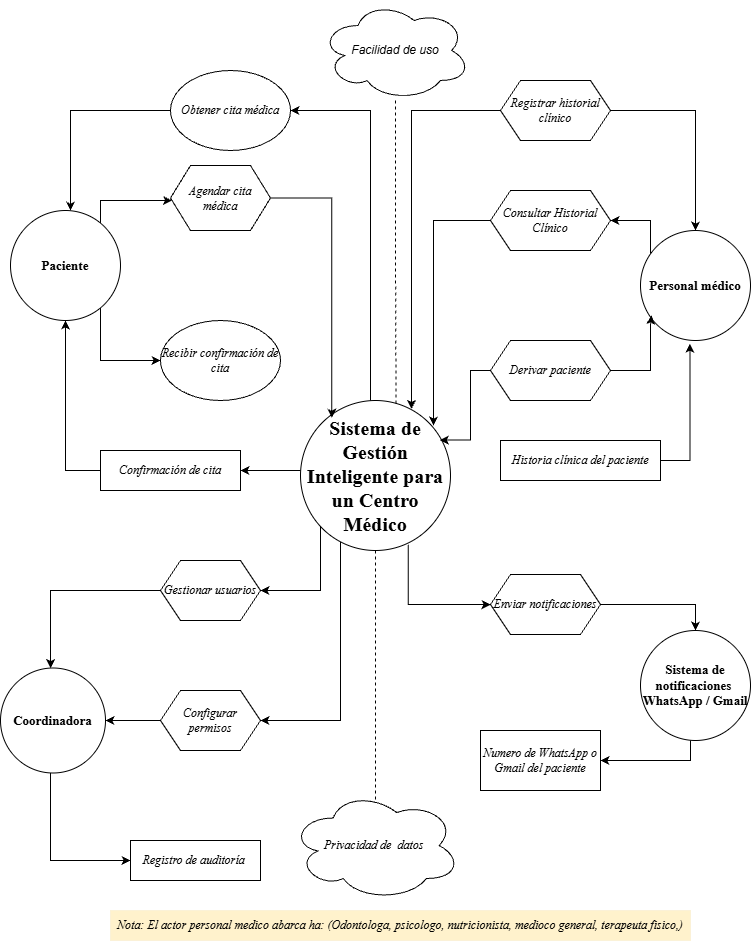
\includegraphics[width=0.75\textwidth]{Diagrama_SD.png}
		\caption{Diagrama del modelo de dependencia estratégica (Strategic Dependency Model, SD)}
		\label{fig:sd-4}
	\end{figure}
	
	
	\begin{quote}
		Diagrama SD elaborado con draw.io que representa las dependencias estratégicas entre los actores \textbf{Paciente}, \textbf{Personal médico}, \textbf{Coordinadora} y \textbf{Sistema de notificaciones WhatsApp/Gmail}, con el \textbf{Sistema de Gestión Inteligente para un Centro Médico} como nodo central. Incluye dependencias de tarea (Agendar cita médica, Registrar historial clínico, Derivar paciente, Gestionar usuarios, Enviar notificaciones), de recurso (Confirmación de cita, Historia clínica del paciente, Número de WhatsApp o Gmail del paciente, Registro de auditoría) y metas blandas (Facilidad de uso, Privacidad de datos). Nota del diagrama: el actor ``personal médico'' abarca a Odontóloga, Psicólogo, Nutricionista, Médico general y Terapeuta físico.
		
	\end{quote}
	
	\textbf{ --- Strategic Rationale Model (SR)}
	
	\begin{figure}[H]
		\centering
		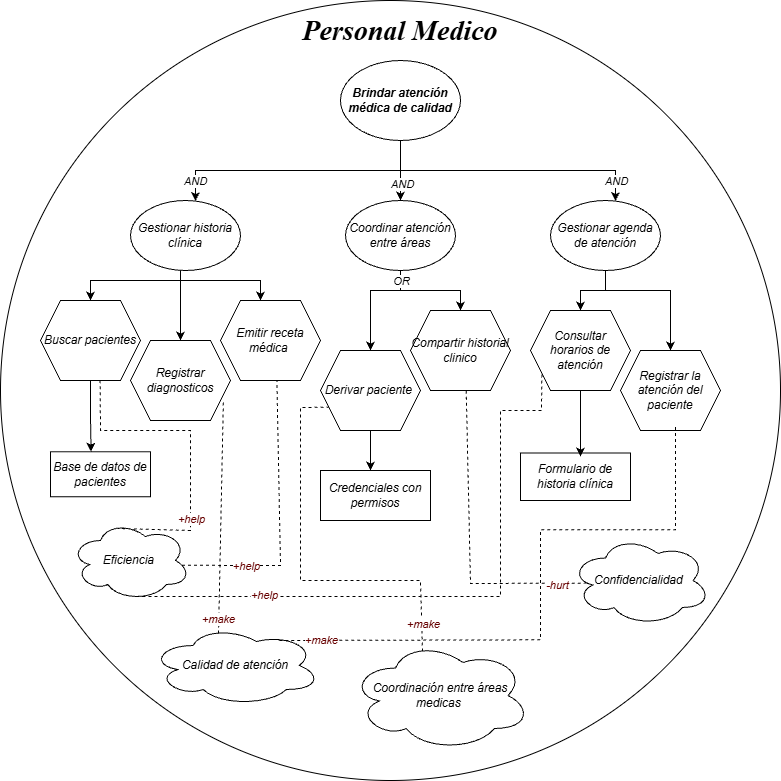
\includegraphics[width=0.75\textwidth]{Diagrama_SR.png}
		\caption{Diagrma de Modelo de racionalidad estratégica "Strategic Rationale Model (SR)" }
		\label{fig:sd-4}
	\end{figure}
	
	\begin{quote}
		Diagrama SR que muestra la descomposición interna de la meta raíz \textbf{``Brindar atención médica de calidad''} del actor Personal Médico en tres submetas unidas por AND: \emph{Gestionar historia clínica}, \emph{Coordinar atención entre áreas} y \emph{Gestionar agenda de atención}. Cada submeta se descompone en tareas (Buscar pacientes, Registrar diagnósticos, Emitir receta médica, Derivar paciente / Compartir historial clínico, Consultar horarios de atención, Registrar la atención del paciente), asociadas a recursos (Base de datos de pacientes, Credenciales con permisos, Formulario de historia clínica). Se representan enlaces de contribución (\texttt{+help}, \texttt{+make}, \texttt{-hurt}) hacia los softgoals \textbf{Eficiencia}, \textbf{Calidad de atención}, \textbf{Coordinación entre áreas médicas} y \textbf{Confidencialidad}.
		
	\end{quote}
	
	\subsection{ Restricciones generales}
	
	\begin{itemize}
		\tightlist
		\item
		El sistema deberá cumplir con la Ley Orgánica de Protección de Datos Personales del Ecuador (LOPDP) vigente desde 2021 \cite{loppd}.
		\item
		El desarrollo se realizará con las herramientas y tecnologías disponibles para el equipo.
		\item
		La infraestructura de Inteligencia Artificial necesaria para el asistente virtual (RF-16) no está disponible en su totalidad en esta fase; su incorporación será progresiva. Por su naturaleza de sistema de IA orientado a usuarios finales en un contexto sanitario, deberá satisfacer requisitos de transparencia, explicabilidad, supervisión humana y gestión del riesgo, en concordancia con las recomendaciones de la OMS, la literatura médica y el marco regulatorio europeo \cite{whoai2021,topol2019,rajkomar2019,euaiact2024}.
		\item
		El sistema deberá operar correctamente en el horario laboral del centro médico (07h00--18h00, lunes a viernes).
		\item
		El repositorio de código y evidencias se gestionará obligatoriamente en GitHub conforme a la estructura definida en el Apéndice E.
	\end{itemize}
	
	\subsection{ Supuestos y dependencias}
	
	\begin{itemize}
		\tightlist
		\item
		Se asume que el Centro Médico cuenta con conexión a internet estable durante el horario de atención.
		\item
		Se asume la disponibilidad de los pacientes para registrar y mantener actualizado un número de WhatsApp o correo electrónico de contacto.
		\item
		El envío de notificaciones depende de la disponibilidad de la API externa de WhatsApp Business o del servidor SMTP de correo.
		\item
		Se asume que el personal administrativo asignará los permisos de acceso por rol de forma oportuna tras la implementación.
	\end{itemize}
	
	
	
	\section{ Especificación de requisitos}
	
	\subsection{ Interfaces externas y mockups}
	
	A continuación, se describen las pantallas principales del sistema (interfaz de usuario), así como las interfaces de hardware y software identificadas. Cada pantalla se vincula explícitamente a los requisitos funcionales (RF) que soporta. Los mockups detallados de baja/alta fidelidad se encuentran en el repositorio del proyecto, carpeta \texttt{/diagramas/mockups/}; esta sección documenta su especificación funcional.
	
	\subsubsection{ Interfaces de usuario}
	
	
	
	\begin{longtable}{p{0.20\textwidth} p{0.12\textwidth} p{0.45\textwidth} p{0.13\textwidth}}
		
		\toprule
		\textbf{Pantalla} &
		\textbf{Fidelidad} &
		\textbf{Elementos principales} &
		\textbf{RF relacionados} \\
		\midrule
		\endhead
		
		%---------------------------------------------------------
		Inicio de sesión &
		Alta &
		Campos para usuario o correo y contraseña, opción para mostrar u ocultar la
		contraseña, recuperación de acceso, mensajes de error y botón para iniciar
		sesión. El rol no deberá ser seleccionado manualmente, sino determinado según
		la cuenta autenticada. &
		RF-09 \\
		
		%---------------------------------------------------------
		Panel principal &
		Alta &
		Menú de módulos habilitados según el rol, resumen de actividades, citas,
		pacientes pendientes, derivaciones, alertas, notificaciones y acceso al perfil
		del usuario. &
		Por normalizar \\
		
		%---------------------------------------------------------
		Gestión de pacientes &
		Alta &
		Buscador por cédula, nombres, apellidos o número de historia clínica; formulario
		de registro; actualización de información; detección de posibles duplicados y
		consulta de datos generales. &
		RF-01 \\
		
		%---------------------------------------------------------
		Recepción y Recaudación &
		Alta &
		Búsqueda o registro del paciente, selección del servicio, asignación de turno,
		registro del valor, método de pago, emisión del comprobante y envío del paciente
		al área de Enfermería. &
		RF-20, RF-21 \\
		
		%---------------------------------------------------------
		Agenda de citas &
		Alta &
		Selector de paciente, área médica y profesional; calendario de disponibilidad,
		horarios, duración de consulta, confirmación, cancelación, reagendamiento,
		inasistencia y lista de espera. &
		RF-02, RF-13 \\
		
		%---------------------------------------------------------
		Gestión de turnos &
		Media &
		Calendario por área y profesional, cupo máximo, modalidad de atención, orden de
		llegada, prioridad clínica, tiempo de tolerancia y estado del turno. &
		RF-17, RF-23,
		RF-24, RF-25 \\
		
		%---------------------------------------------------------
		Registro de signos vitales &
		Alta &
		Búsqueda del paciente, peso, talla, temperatura, presión arterial, frecuencia
		cardíaca, frecuencia respiratoria, saturación de oxígeno, glucosa y
		observaciones de Enfermería. &
		Por normalizar \\
		
		%---------------------------------------------------------
		Historia clínica electrónica &
		Alta &
		Datos generales, antecedentes personales y familiares, alergias, signos vitales,
		atenciones previas, diagnósticos, tratamientos, recetas, derivaciones,
		documentos y línea de tiempo clínica. &
		RF-01, RF-03 \\
		
		%---------------------------------------------------------
		Atención y evolución clínica &
		Alta &
		Motivo de consulta, anamnesis, observaciones, diagnóstico, tratamiento, notas de
		evolución, profesional responsable, fecha, hora y cierre de atención. &
		RF-03 \\
		
		%---------------------------------------------------------
		Seguimiento de Terapia Física &
		Alta &
		Registro por sesión, presión arterial, diagnóstico inicial, tratamiento,
		observaciones, notas de evolución y comparación cronológica del progreso del
		paciente. &
		Por normalizar \\
		
		%---------------------------------------------------------
		Seguimiento nutricional &
		Alta &
		Peso, talla, índice de masa corporal, circunferencia de cintura, circunferencia
		braquial, grasa corporal, grasa visceral, masa muscular, valores bioquímicos,
		diagnóstico nutricional y plan alimentario. &
		Por normalizar \\
		
		%---------------------------------------------------------
		Gestión de derivaciones &
		Alta &
		Paciente, área de origen, área de destino, profesional, motivo, prioridad,
		información clínica adjunta, fecha, estado, aceptación o rechazo y seguimiento
		de la derivación. &
		Por normalizar \\
		
		%---------------------------------------------------------
		Emisión de receta médica &
		Alta &
		Diagnóstico relacionado, selector de medicamento, presentación, concentración,
		dosis, frecuencia, duración, cantidad, vía de administración, indicaciones,
		vista previa y envío a Enfermería. &
		RF-04 \\
		
		%---------------------------------------------------------
		Gestión de inventario &
		Alta &
		Tabla de medicamentos e insumos, nombre, descripción de uso, presentación,
		concentración, lote, cantidad, stock mínimo, fecha de fabricación, fecha de
		vencimiento, entradas, salidas y alertas. &
		RF-15 \\
		
		%---------------------------------------------------------
		Entrega de medicamentos &
		Alta &
		Búsqueda de receta, identificación del paciente, medicamento, lote, cantidad
		prescrita, cantidad entregada, responsable, fecha, observaciones y actualización
		automática del inventario. &
		Por normalizar \\
		
		%---------------------------------------------------------
		Panel de reportes &
		Media &
		Filtros por rango de fechas, área, profesional, tipo de atención y categoría;
		tablas, indicadores, gráficos, vista previa, exportación e impresión. &
		RF-08 \\
		
		%---------------------------------------------------------
		Gestión de usuarios y permisos &
		Media &
		Listado de usuarios, creación de cuentas, asignación de roles y áreas,
		activación o desactivación, restablecimiento de contraseña, permisos e historial
		de cambios. &
		RF-09, RF-10 \\
		
		%---------------------------------------------------------
		Auditoría del sistema &
		Media &
		Filtros por usuario, fecha, módulo y acción; detalle de accesos y cambios;
		identificación del elemento afectado y exportación autorizada de registros. &
		Por normalizar \\
		
		%---------------------------------------------------------
		Notificaciones &
		Media &
		Bandeja de avisos, tipo de notificación, destinatario, fecha, estado de lectura,
		estado de envío y acceso a la funcionalidad relacionada. &
		RF-11 \\
		
		%---------------------------------------------------------
		Perfil del personal médico &
		Alta &
		Datos personales y profesionales, especialidad, número de registro profesional,
		área asignada, horarios, estado, datos de contacto e historial de turnos. &
		RF-18, RF-19 \\
		
		%---------------------------------------------------------
		Asistente virtual &
		Baja
		(prototipo) &
		Caja de conversación, preguntas frecuentes, orientación sobre horarios,
		servicios y uso del sistema. No deberá emitir diagnósticos ni recomendaciones
		médicas autónomas. &
		RF-16 \\
		
		\bottomrule
		
	\end{longtable}
	
	\begin{figure}[H]
		\centering
		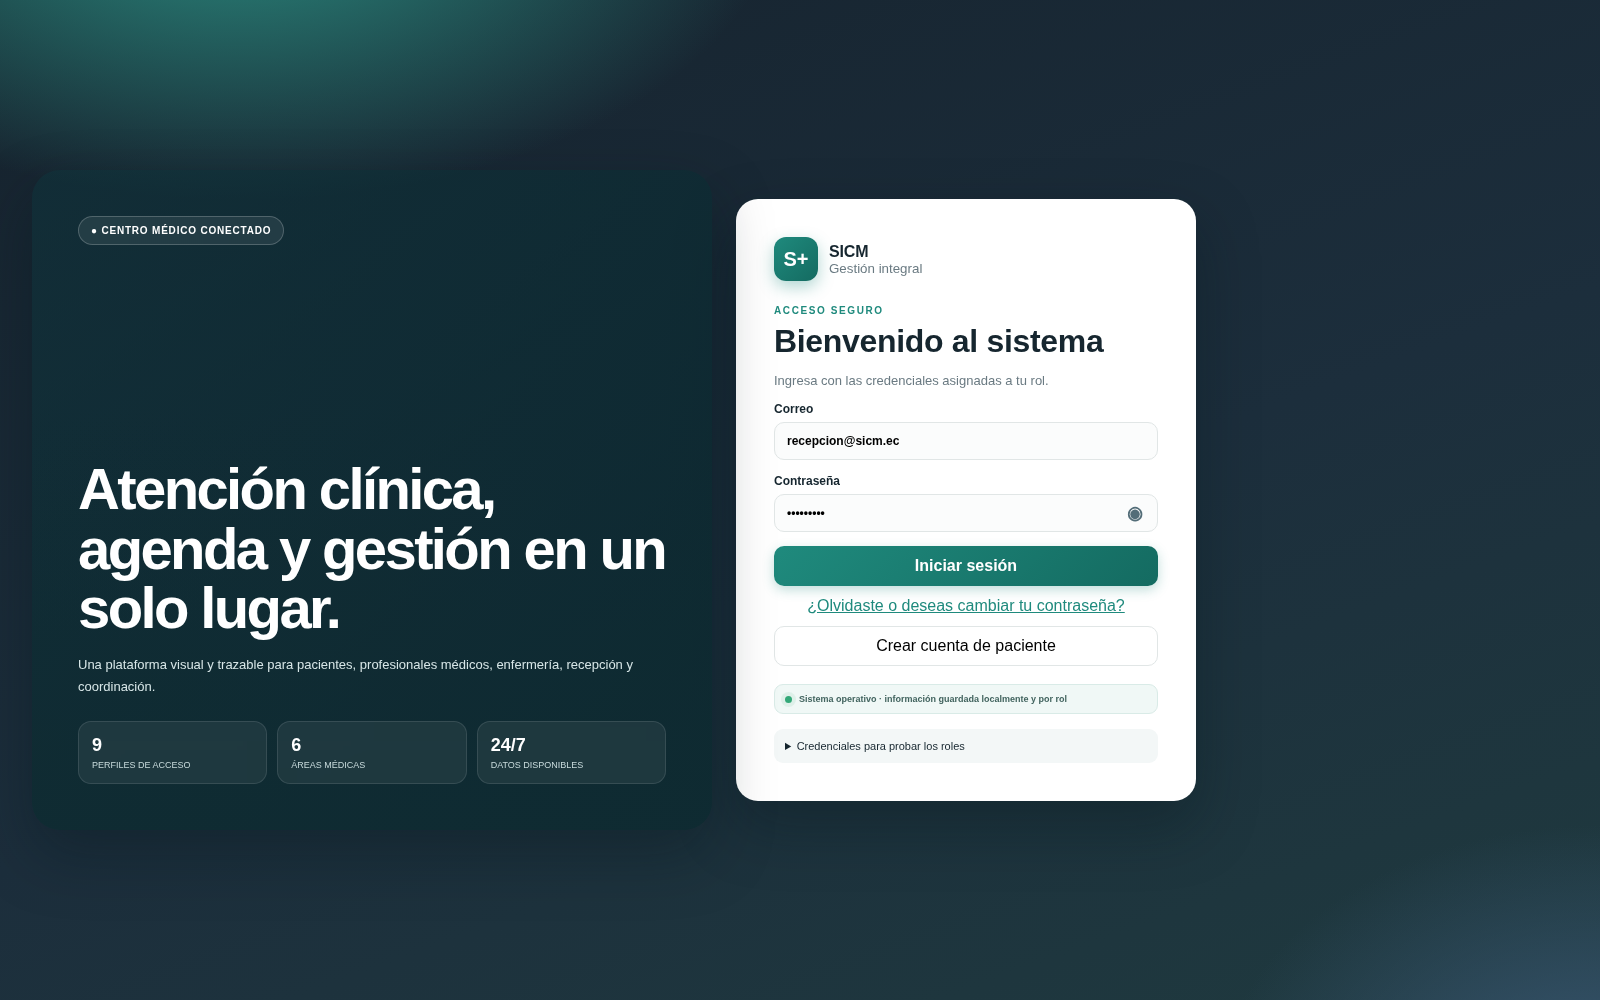
\includegraphics[width=0.49\textwidth]{I_Inicio_Sesion.png}
		\caption{Interfaz de Inicio de Sesion para el ingreso al sistema segun su rol asignado, generada a partir de los requisitos no funcionales. }
		\label{fig:sd-1}
	\end{figure}
	
	\begin{figure}[H]
		\centering
		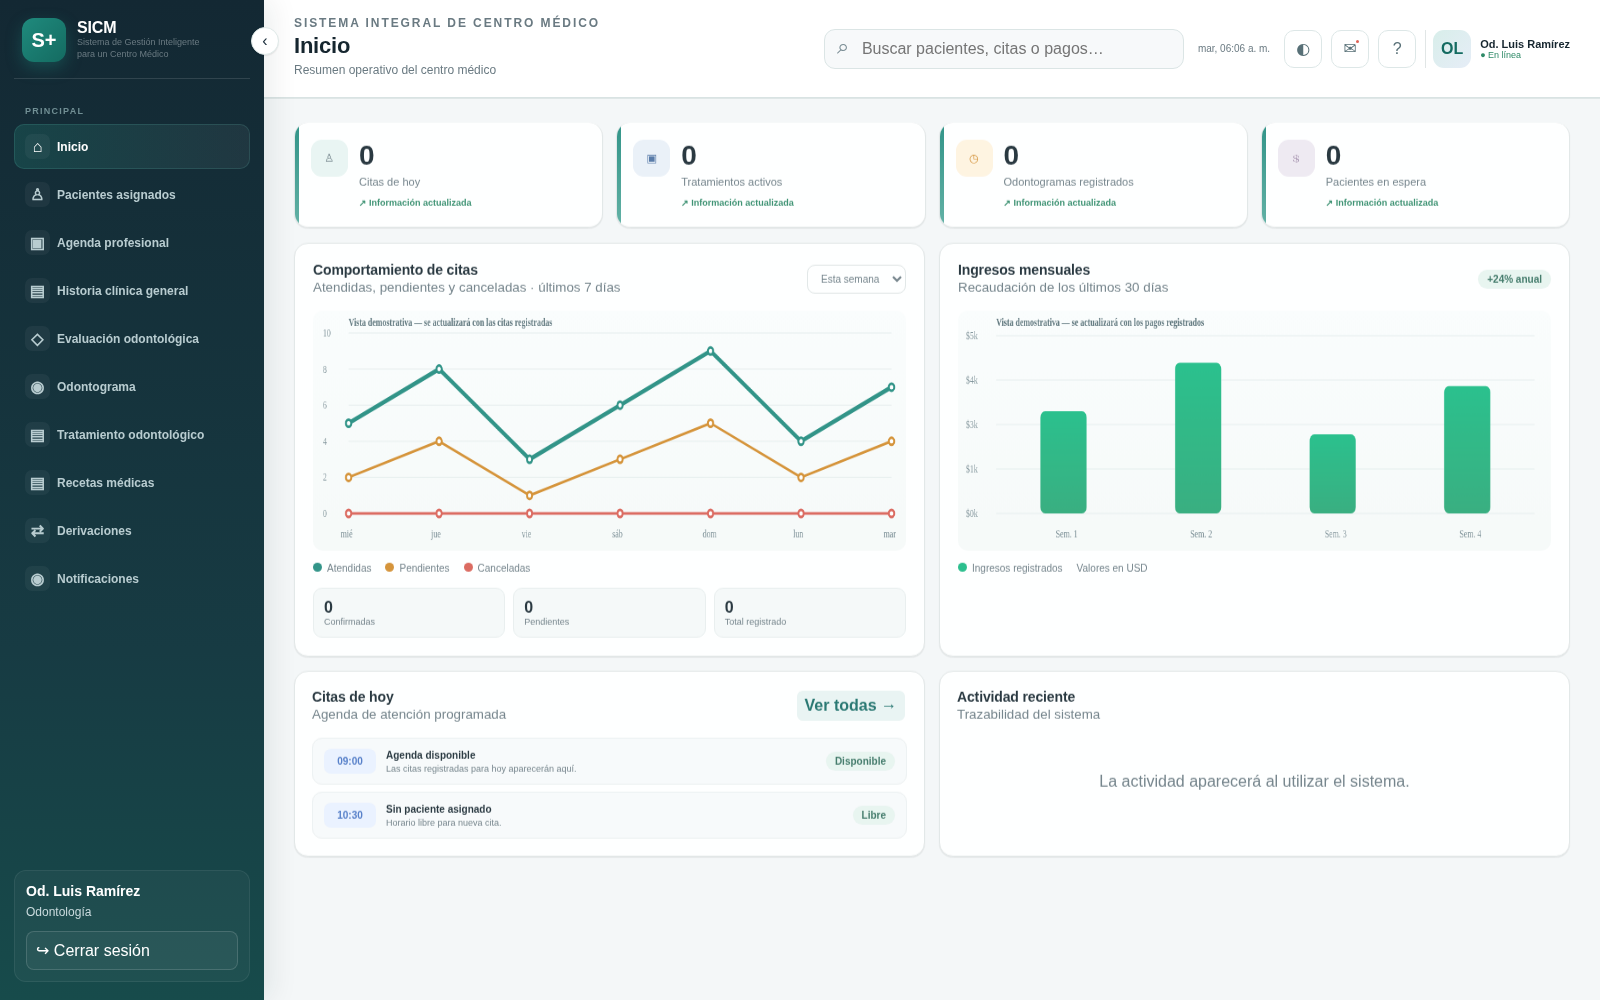
\includegraphics[width=0.75\textwidth]{I_Odontologia.png}
		\caption{Interfaz de navegación del area de odontologia, generada apartir de los requisitos funcionales. }
		\label{fig:sd-2}
	\end{figure}
	
	\begin{figure}[H]
		\centering
		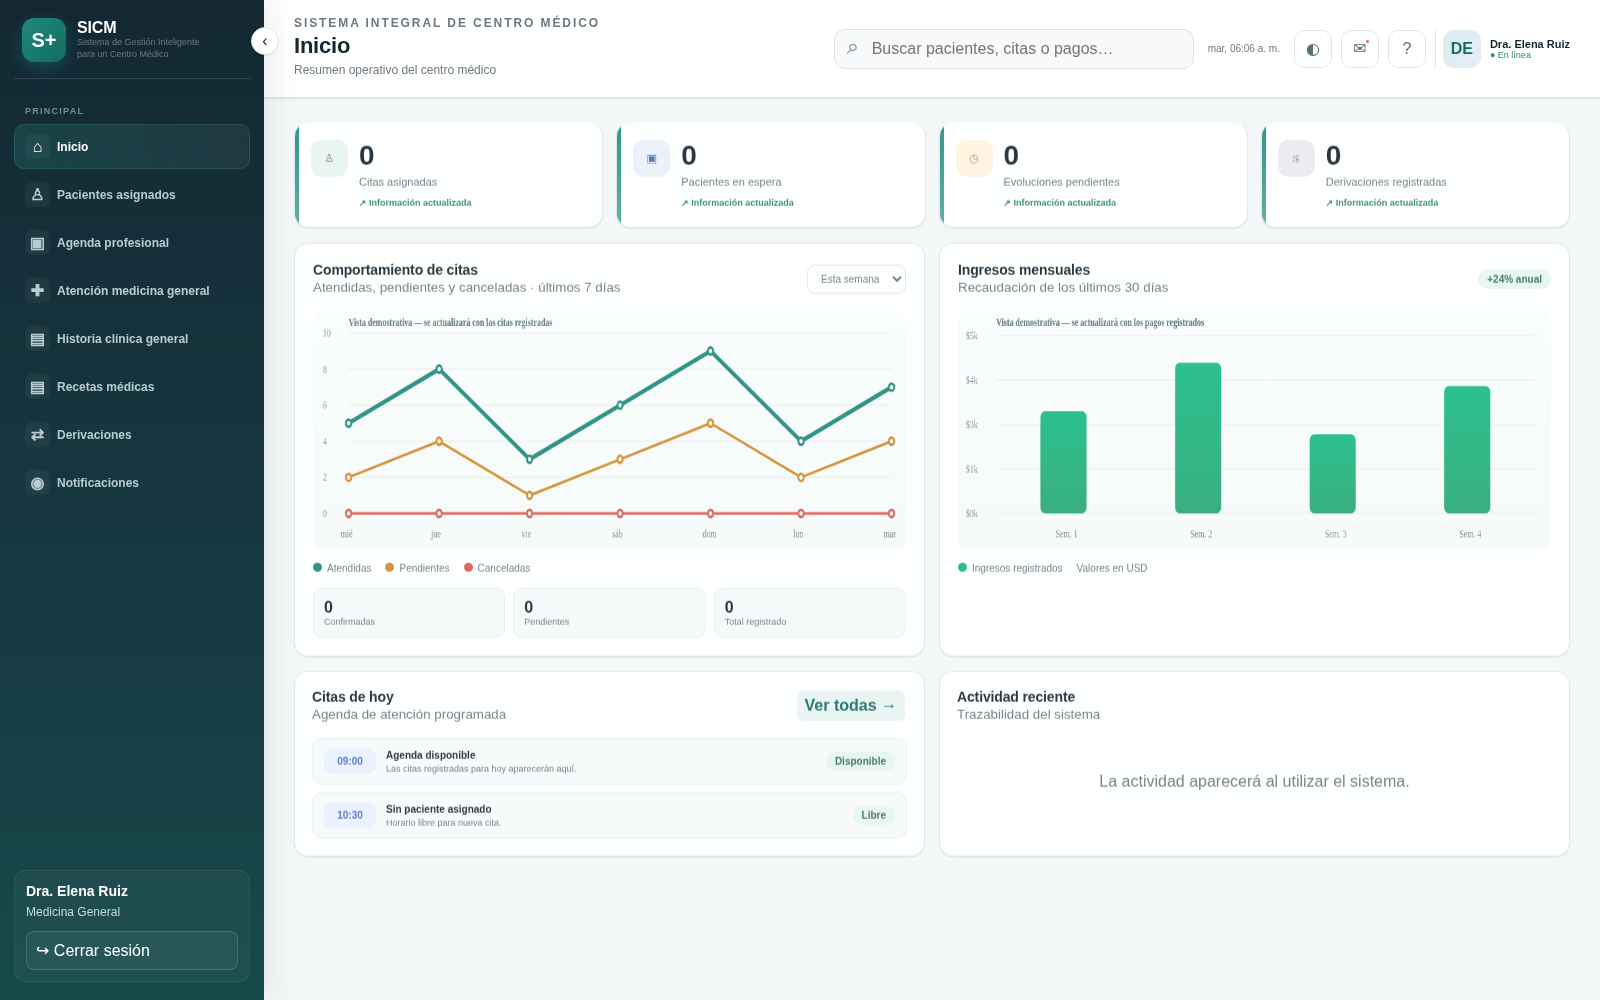
\includegraphics[width=0.75\textwidth]{I_MedicoGeneral.png}
		\caption{Interfaz de navegación del area de Medicina General, generada apartir de los requisitos funcionales. }
		\label{fig:sd-3}
	\end{figure}
	
	\begin{figure}[H]
		\centering
		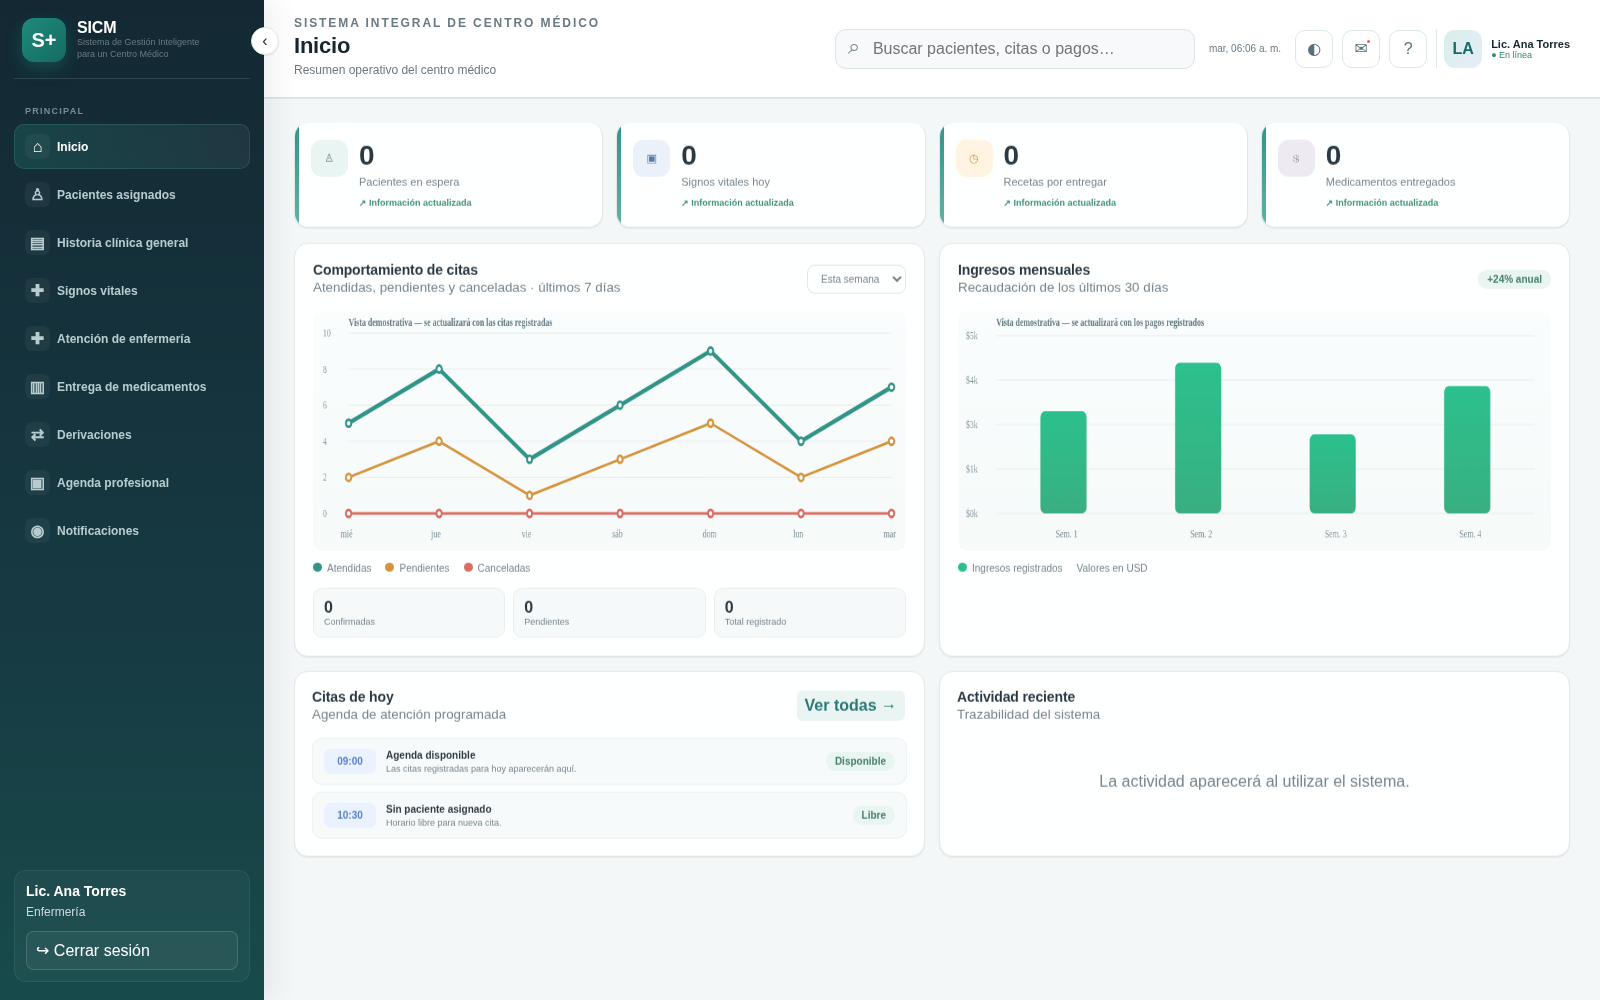
\includegraphics[width=0.75\textwidth]{I_Enfermeria.png}
		\caption{Interfaz de navegación del area de Enfermeria, generada apartir de los requisitos funcionales }
		\label{fig:sd-4}
	\end{figure}
	
	
	En el repositorio se encuentran disponibles un total de 29 mockups correspondientes a las interfaces más relevantes y representativas del sistema. Estos mockups cubren las principales funcionalidades y procesos identificados durante el levantamiento de requisitos; sin embargo, no incluyen la totalidad de las pantallas. Las interfaces restantes serán desarrolladas, refinadas e incorporadas en la versión final para la próxima entrega.
	
	\subsubsection{ Interfaces de hardware}
	
	\begin{longtable}{p{0.18\textwidth} p{0.32\textwidth} p{0.42\textwidth}}
		
		
		
		\toprule
		\textbf{Dispositivo} &
		\textbf{Forma de interacción} &
		\textbf{Uso previsto dentro del sistema} \\
		\midrule
		\endhead
		
		\bottomrule
		\endlastfoot
		
		Computadora de escritorio &
		Acceso mediante navegador web, teclado, ratón y monitor. &
		Uso principal del sistema en Recepción, Recaudación, Enfermería,
		Coordinación y áreas clínicas. \\
		
		Computadora portátil &
		Acceso mediante navegador web y conexión a la red institucional. &
		Uso por personal autorizado para consultar o registrar información dentro de
		las instalaciones. \\
		
		Monitor o pantalla &
		Presentación de formularios, expedientes, calendarios, tablas, reportes,
		alertas y notificaciones. &
		Visualización de las funciones disponibles según el rol del usuario. \\
		
		Teclado &
		Ingreso alfanumérico de datos. &
		Registro de pacientes, historias clínicas, diagnósticos, tratamientos,
		medicamentos, pagos y observaciones. \\
		
		Ratón  &
		Selección de menús, campos, fechas, botones y opciones. &
		Navegación general por la interfaz del sistema. \\
		
		Impresora &
		Comunicación mediante los controladores del sistema operativo. &
		Impresión autorizada de recetas, comprobantes, turnos, reportes y otros
		documentos institucionales. \\
		
		
		Dispositivo móvil o tableta &
		Acceso mediante navegador compatible y diseño adaptable. &
		Consulta de información, notificaciones o funciones específicas autorizadas.
		No se considerará el medio principal de operación en la primera versión. \\
		
		Servidor &
		Alojamiento de la aplicación, base de datos, archivos y servicios internos. &
		Procesamiento centralizado, almacenamiento, autenticación, auditoría y
		generación de respaldos. \\
		
		Dispositivo de respaldo &
		Almacenamiento local o externo autorizado. &
		Conservación de copias de seguridad de la base de datos y documentos del
		sistema. \\
		
	\end{longtable}
	
	\subsubsection{ Interfaces de software}
	
	\begin{longtable}{p{0.24\textwidth} p{0.31\textwidth} p{0.40\textwidth}}
		
		
		\toprule
		\textbf{Componente o servicio} &
		\textbf{Interacción prevista} &
		\textbf{Condiciones principales} \\
		\midrule
		\endhead
		
		\bottomrule
		\endlastfoot
		
		Navegador web &
		Presentación de la interfaz y comunicación con el servidor de aplicaciones. &
		Deberá admitir tecnologías web actuales, coneiones seguras, formularios,
		tablas, calendarios y diseño adaptable. \\
		
		Servidor web &
		Recepción de solicitudes de los clientes y entrega de contenido. &
		Deberá operar mediante HTTPS en el ambiente de producción. \\
		
		Servidor de aplicaciones &
		Ejecución de la lógica de negocio del sistema. &
		Deberá validar permisos, procesar operaciones, aplicar reglas de negocio y
		comunicarse con la base de datos. \\
		
		Motor de base de datos &
		Almacenamiento estructurado de pacientes, citas, historias clínicas,
		medicamentos, inventario, usuarios, pagos y auditoría. &
		Deberá mantener integridad, relaciones, transacciones, restricciones y copias de
		seguridad. \\
		
		Sistema operativo del servidor &
		Ejecución de los servicios necesarios para alojar el SICM. &
		La plataforma específica deberá definirse en la arquitectura técnica aprobada. \\
		
		Servicio de autenticación &
		Validación de identidad, credenciales, sesiones y permisos. &
		Podrá formar parte del propio SICM o integrarse con un servicio institucional,
		si este se encuentra disponible. \\
		
		Servicio de correo electrónico &
		Envío de recuperación de contraseña, confirmaciones, recordatorios,
		comprobantes y notificaciones. &
		El envío deberá realizarse mediante una cuenta institucional o proveedor
		autorizado; no deberá limitarse exclusivamente a Gmail. \\
		
		Servicio de mensajería &
		Envío opcional de avisos relacionados con citas y disponibilidad. &
		Podrá utilizarse una API institucional o un servicio aprobado, como WhatsApp
		Business, sin que sea obligatorio para las funciones clínicas principales. \\
		
		Servicio de generación de documentos &
		Creación de recetas, comprobantes, reportes y archivos exportables. &
		Los formatos deberán definirse en los requisitos funcionales; como mínimo podrá
		considerarse PDF y, cuando corresponda, hojas de cálculo. \\
		
		Servicio de almacenamiento de archivos &
		Conservación de documentos adjuntos, imágenes y archivos generados. &
		Los archivos deberán asociarse al registro correspondiente y protegerse según
		los permisos del usuario. \\
		
		Servicio de respaldo &
		Generación y conservación de copias de la base de datos y documentos. &
		Deberá ejecutarse con la periodicidad definida en los requisitos no funcionales
		y permitir procedimientos de recuperación. \\
		
		Servicio de auditoría &
		Registro de acciones realizadas por los usuarios y procesos del sistema. &
		Deberá registrar usuario, acción, módulo, fecha, hora y elemento afectado, sin
		permitir modificación ordinaria de los registros. \\
		
		Servicio de exportación &
		Conversión de datos filtrados a formatos autorizados. &
		La exportación deberá respetar los permisos y registrar la operación cuando se
		incluyan datos sensibles. \\
		
	\end{longtable}
	
	\subsection{ Requisitos funcionales}
	
	Cada requisito funcional se documenta con ocho atributos: identificador, nombre, descripción, actor/origen, entradas/salidas, precondiciones/postcondiciones, prioridad MoSCoW y criterio de verificación, conforme a ISO/IEC/IEEE 29148:2018 \cite{iso29148}. El catálogo vigente contiene exactamente 40 requisitos funcionales, numerados consecutivamente desde RF-01 hasta RF-40. La redacción verificable y la trazabilidad bidireccional se apoyan además en trabajos clásicos de ingeniería de requisitos \cite{nuseibeh2000,davis1993,gotel1994,ramesh2001,clelandhuang2003}.
	
	\subsubsection{RF-01 --- Registrar historia clínica digital}
	
	
	\begin{longtable}{p{0.28\textwidth} p{0.65\textwidth}}
		
		\toprule
		\textbf{Atributo} & \textbf{Detalle} \\
		\midrule
		\endhead
		
		Identificador & RF-01 \\		
		Nombre & Registrar historia clínica digital \\		
		Descripción &
		El sistema deberá permitir registrar y consultar historias clínicas digitales de los pacientes, incluyendo información personal, antecedentes médicos, alergias, enfermedades y medicamentos. \\
		Actor / Origen (evidencia) &
		Personal médico / Acta de entrevista N°1 (EV-01) \\		
		Entradas / Salidas &
		Entrada: datos personales y clínicos del paciente. Salida: historia clínica registrada con ID único. \\
		Precondiciones / Postcondiciones &
		El médico/enfermera está autenticado con permisos activos / La historia clínica queda almacenada en BD\_CentroMedico \\
		
		Prioridad (MoSCoW) &		Must \\
		Criterio de verificación &
		Verificar que el registro creado sea recuperable mediante búsqueda por cédula en \(\leq\) 2 segundos. Incluye la digitalización progresiva de los procesos actualmente soportados en papel (historiales, recetas, formularios de derivación): al menos el 80\,\% de los formularios físicos identificados deben tener equivalente digital al cierre del proyecto (antes RF-14, fusionado aquí por tratarse de la misma meta de digitalización). \\
		
		\bottomrule
		
	\end{longtable}
	
	\subsubsection{RF-02 --- Agendar cita médica}
	
	\begin{longtable}{p{0.28\textwidth} p{0.65\textwidth}}
		
		\toprule
		\textbf{Atributo} & \textbf{Detalle} \\
		\midrule
		\endhead
		
		Identificador & RF-02 \\
		Nombre & Agendar cita médica \\
		Descripción & El sistema deberá gestionar el agendamiento de citas médicas, permitiendo al paciente seleccionar área médica y horario disponible. \\
		Actor / Origen (evidencia) & Paciente / Acta de entrevista N°1, Cuestionario digital (EV-01, EV-02) \\
		Entradas / Salidas & Entrada: área médica, fecha y turno. Salida: cita registrada y confirmación en pantalla. \\
		Precondiciones / Postcondiciones & El paciente está autenticado en el sistema / La cita queda registrada en BD\_CentroMedico y el paciente recibe confirmación \\
		Prioridad (MoSCoW) & Must \\
		Criterio de verificación & El sistema debe confirmar el agendamiento en pantalla en \(\leq\) 3 segundos (ver US-1). Incluye el agendamiento por área para las áreas que lo requieren (por ejemplo, terapia física), registrando fecha, hora y profesional asignado, además de la atención por orden de turno usada en medicina general (antes RF-36, fusionado por ser el mismo flujo de agendamiento visto por área). \\
		
		\bottomrule
		
	\end{longtable}
	
	\subsubsection{RF-03 --- Buscar pacientes por criterios}
	
	\begin{longtable}{p{0.28\textwidth} p{0.65\textwidth}}
		
		\toprule
		\textbf{Atributo} & \textbf{Detalle} \\
		\midrule
		\endhead
		
		Identificador & RF-03 \\
		Nombre & Buscar pacientes por criterios \\
		Descripción & El sistema deberá permitir la búsqueda rápida de pacientes mediante nombre, iniciales o cédula. \\
		Actor / Origen (evidencia) & Médico / Acta de entrevista N°1 (EV-01) \\
		Entradas / Salidas & Entrada: cédula o iniciales de nombre. Salida: ficha del paciente encontrado o mensaje de no encontrado. \\
		Precondiciones / Postcondiciones & El usuario tiene sesión activa con permisos sobre el módulo de historial / El sistema muestra el historial correspondiente o un mensaje de no registrado \\
		Prioridad (MoSCoW) & Must \\
		Criterio de verificación & El resultado de búsqueda debe mostrarse en \(\leq\) 2 segundos (ver US-2). La búsqueda por número de cédula debe retornar el expediente correspondiente en \(\leq\) 3 segundos, verificado con al menos 20 expedientes de prueba (antes RF-27, fusionado por ser un criterio de búsqueda dentro del mismo RF). \\
		
		\bottomrule
		
	\end{longtable}
	
	\subsubsection{RF-04 --- Emitir receta médica}
	
	\begin{longtable}{p{0.28\textwidth} p{0.65\textwidth}}
		
		\toprule
		\textbf{Atributo} & \textbf{Detalle} \\
		\midrule
		\endhead
		
		Identificador & RF-04 \\
		Nombre & Emitir receta médica \\
		Descripción & El sistema deberá permitir registrar recetas médicas asociadas al historial clínico de cada paciente, indicando medicamento, cantidad e indicaciones. \\
		Actor / Origen (evidencia) & Médico (Odontología / Medicina General) / Acta de entrevista N°1 (EV-01) \\
		Entradas / Salidas & Entrada: medicamento, cantidad, indicaciones. Salida: receta registrada y vinculada al historial. \\
		Precondiciones / Postcondiciones & El médico tiene una atención activa con el paciente / La receta queda registrada en BD\_CentroMedico vinculada al historial del paciente \\
		Prioridad (MoSCoW) & Must \\
		Criterio de verificación & La receta debe quedar visible en el historial del paciente inmediatamente después de su emisión (ver US-3). \\
		
		\bottomrule
		
	\end{longtable}
	
	\subsubsection{RF-05 --- Actualizar información clínica}
	
	\begin{longtable}{p{0.28\textwidth} p{0.65\textwidth}}
		
		\toprule
		\textbf{Atributo} & \textbf{Detalle} \\
		\midrule
		\endhead
		
		Identificador & RF-05 \\
		Nombre & Actualizar información clínica \\
		Descripción & El sistema deberá permitir actualizar la información clínica de un paciente sin necesidad de volver a registrar todos los datos. \\
		Actor / Origen (evidencia) & Médico / Acta de entrevista N°1 (EV-01) \\
		Entradas / Salidas & Entrada: campos clínicos modificados. Salida: historial actualizado con marca de fecha/hora. \\
		Precondiciones / Postcondiciones & El médico ha buscado y seleccionado al paciente / El historial clínico refleja los nuevos datos manteniendo el registro histórico previo \\
		Prioridad (MoSCoW) & Should \\
		Criterio de verificación & El sistema debe registrar la fecha y el usuario que realizó cada modificación (ver US-5). \\
		
		\bottomrule
		
	\end{longtable}
	
	\subsubsection{RF-06 --- Cancelar / modificar cita médica}
	
	\begin{longtable}{p{0.28\textwidth} p{0.65\textwidth}}
		
		\toprule
		\textbf{Atributo} & \textbf{Detalle} \\
		\midrule
		\endhead
		
		Identificador & RF-06 \\
		Nombre & Cancelar / modificar cita médica \\
		Descripción & El sistema deberá permitir al paciente cancelar o reprogramar una cita médica previamente agendada. \\
		Actor / Origen (evidencia) & Paciente / Acta de entrevista N°1 (EV-01) \\
		Entradas / Salidas & Entrada: selección de la cita, motivo (opcional). Salida: cita cancelada/reprogramada y turno liberado. \\
		Precondiciones / Postcondiciones & El paciente tiene al menos una cita activa / La cita cambia de estado y el turno queda disponible para otros pacientes \\
		Prioridad (MoSCoW) & Must \\
		Criterio de verificación & El sistema debe confirmar la cancelación y liberar el cupo en \(\leq\) 2 segundos (ver US-4). Incluye la reprogramación o cancelación de citas por área, dejando constancia del cambio (fecha original y nueva fecha) (antes RF-37, fusionado por ser la misma acción sobre la cita vista por área). \\
		
		\bottomrule
		
	\end{longtable}
	
	\subsubsection{RF-07 --- Compartir información clínica entre áreas}
	
	\begin{longtable}{p{0.28\textwidth} p{0.65\textwidth}}
		
		\toprule
		\textbf{Atributo} & \textbf{Detalle} \\
		\midrule
		\endhead
		
		Identificador & RF-07 \\
		Nombre & Compartir información clínica entre áreas \\
		Descripción & El sistema deberá permitir compartir información clínica relevante entre las distintas áreas médicas autorizadas mediante derivación formal. \\
		Actor / Origen (evidencia) & Personal médico / Acta de negociación N°1 (EV-04) \\
		Entradas / Salidas & Entrada: paciente, área destino, motivo de derivación. Salida: derivación registrada y notificada al área receptora. \\
		Precondiciones / Postcondiciones & El paciente tiene una atención activa y existe una relación formal con el área de destino / La derivación queda registrada y visible para el área receptora \\
		Prioridad (MoSCoW) & Should \\
		Criterio de verificación & El área receptora debe poder consultar el historial parcial del paciente derivado, conforme al RNF de control de acceso. \\
		
		\bottomrule
		
	\end{longtable}
	
	\subsubsection{RF-08 --- Generar reportes de atención}
	
	\begin{longtable}{p{0.28\textwidth} p{0.65\textwidth}}
		
		\toprule
		\textbf{Atributo} & \textbf{Detalle} \\
		\midrule
		\endhead
		
		Identificador & RF-08 \\
		Nombre & Generar reportes de atención \\
		Descripción & El sistema deberá generar reportes diarios y mensuales de atención por especialidad médica, con filtros por rango de fechas y categoría. \\
		Actor / Origen (evidencia) & Coordinadora / Administrador / Acta de entrevista N°1 (EV-01) \\
		Entradas / Salidas & Entrada: rango de fechas, categoría. Salida: reporte visual/exportable de atenciones. \\
		Precondiciones / Postcondiciones & El administrador está autenticado con permisos de reportes / El sistema muestra el reporte solicitado o notifica que no existen atenciones registradas \\
		Prioridad (MoSCoW) & Should \\
		Criterio de verificación & El reporte debe generarse en \(\leq\) 5 segundos para rangos de hasta 1 año. \\
		
		\bottomrule
	\end{longtable}
	
	\subsubsection{RF-09 --- Autenticación de usuarios}
	
	\begin{longtable}{p{0.28\textwidth} p{0.65\textwidth}}
		
		\toprule
		\textbf{Atributo} & \textbf{Detalle} \\
		\midrule
		\endhead
		
		Identificador & RF-09 \\
		Nombre & Autenticación de usuarios \\
		Descripción & El sistema deberá permitir el inicio de sesión de pacientes y personal mediante credenciales, con recuperación de contraseña y notificación de credenciales incorrectas. \\
		Actor / Origen (evidencia) & Todos los actores / Diagrama de CU-12 Iniciar sesión (Figura 4) \\
		Entradas / Salidas & Entrada: usuario y contraseña. Salida: acceso concedido o mensaje de error. \\
		Precondiciones / Postcondiciones & El usuario posee una cuenta activa en el sistema / El usuario accede al módulo correspondiente a su rol \\
		Prioridad (MoSCoW) & Must \\
		Criterio de verificación & El sistema debe bloquear el acceso tras 5 intentos fallidos consecutivos y notificar al usuario. El ciclo de autenticación incluye la recuperación de contraseña mediante enlace temporal y el cierre de sesión con confirmación (funciones consolidadas en este mismo requisito). \\
		\bottomrule
	\end{longtable}
	
	\subsubsection{RF-10 --- Gestionar permisos y roles}
	
	\begin{longtable}{p{0.28\textwidth} p{0.65\textwidth}}
		
		\toprule
		\textbf{Atributo} & \textbf{Detalle} \\
		\midrule
		\endhead
		
		Identificador & RF-10 \\
		Nombre & Gestionar permisos y roles \\
		Descripción & El sistema deberá permitir al administrador otorgar, modificar o revocar permisos de acceso por rol y área médica. \\
		Actor / Origen (evidencia) & Administrador / Diagrama de CU-13 Gestionar Permisos (Figura 5) \\
		Entradas / Salidas & Entrada: usuario, rol, área. Salida: permisos actualizados. \\
		Precondiciones / Postcondiciones & El administrador está autenticado con privilegios de gestión de roles / El usuario afectado obtiene o pierde acceso a los módulos correspondientes \\
		Prioridad (MoSCoW) & Must \\
		Criterio de verificación & Todo cambio de permiso debe quedar registrado en el registro de auditoría (RF-12). Incluye la restricción de visualización del contenido clínico de otras especialidades según el rol (con un usuario de rol ``recepción'', un intento de abrir una nota clínica de otra especialidad debe ser denegado) y la gestión de cuentas de usuario (alta, edición, desactivación) (funciones consolidadas en este mismo requisito). \\
		\bottomrule
	\end{longtable}
	
	\subsubsection{RF-11 --- Enviar notificaciones automáticas}
	
	\begin{longtable}{p{0.28\textwidth} p{0.65\textwidth}}
		
		\toprule
		\textbf{Atributo} & \textbf{Detalle} \\
		\midrule
		\endhead
		
		Identificador & RF-11 \\
		Nombre & Enviar notificaciones automáticas \\
		Descripción & El sistema deberá notificar automáticamente a los pacientes sobre citas agendadas, modificadas o canceladas, vía WhatsApp o correo electrónico. \\
		Actor / Origen (evidencia) & Sistema de Notificaciones / Cuestionario digital (EV-02): 100 \% prefiere WhatsApp \\
		Entradas / Salidas & Entrada: evento de cita (creación/cambio/cancelación). Salida: mensaje enviado y estado de entrega registrado. \\
		Precondiciones / Postcondiciones & El paciente tiene un canal de contacto válido registrado / La notificación se envía y su estado (enviado/fallido) queda registrado \\
		Prioridad (MoSCoW) & Must \\
		Criterio de verificación & El sistema debe registrar el estado de entrega de cada notificación en un máximo de 1 minuto tras el evento (ver CU-14). \\
		\bottomrule
	\end{longtable}
	
	\subsubsection{RF-12 --- Registrar auditoría de acciones}
	
	\begin{longtable}{p{0.28\textwidth} p{0.65\textwidth}}
		
		\toprule
		\textbf{Atributo} & \textbf{Detalle} \\
		\midrule
		\endhead
		
		Identificador & RF-12 \\
		Nombre & Registrar auditoría de acciones \\
		Descripción & El sistema deberá registrar todo acceso y modificación sensible (historial clínico, permisos) con fecha, hora y usuario responsable. \\
		Actor / Origen (evidencia) & Sistema / Acta de negociación N°1 (EV-04) \\
		Entradas / Salidas & Entrada: acción ejecutada por un usuario. Salida: registro de auditoría inmutable. \\
		Precondiciones / Postcondiciones & El usuario ejecuta una acción sobre un módulo auditado / El evento queda almacenado en el registro de auditoría \\
		Prioridad (MoSCoW) & Must \\
		Criterio de verificación & El registro debe ser consultable por el administrador y no editable por ningún rol (ver CU-15). \\
		\bottomrule
	\end{longtable}
	
	\subsubsection{RF-13 --- Consultar disponibilidad de horarios}
	
	\begin{longtable}{p{0.28\textwidth} p{0.65\textwidth}}
		
		\toprule
		\textbf{Atributo} & \textbf{Detalle} \\
		\midrule
		\endhead
		
		Identificador & RF-13 \\
		Nombre & Consultar disponibilidad de horarios \\
		Descripción & El sistema deberá mostrar al paciente los turnos y horarios disponibles por área médica antes de confirmar el agendamiento. \\
		Actor / Origen (evidencia) & Paciente / Diagrama de CU-01 Agendar cita médica (Figura 12) \\
		Entradas / Salidas & Entrada: área médica seleccionada. Salida: lista de horarios disponibles o próximas fechas con cupo. \\
		Precondiciones / Postcondiciones & El paciente ha seleccionado un área médica / El sistema presenta horarios disponibles o sugiere fechas alternativas \\
		Prioridad (MoSCoW) & Must \\
		Criterio de verificación & Si no hay disponibilidad, el sistema debe sugerir automáticamente las próximas 3 fechas con cupo. Incluye informar al paciente (por ejemplo, a través de recepción) los horarios de atención y disponibilidad vigentes de cada área, coincidiendo con la configuración administrada (antes RF-39, fusionado por ser la misma consulta de disponibilidad orientada al paciente). \\
		\bottomrule
	\end{longtable}
	
	\subsubsection{RF-14 --- Digitalizar la documentación clínica}
	\begin{longtable}{p{0.28\textwidth} p{0.65\textwidth}}
		\toprule
		\textbf{Atributo} & \textbf{Detalle} \\
		\midrule
		\endhead
		Identificador & RF-14 \\
		Nombre & Digitalizar la documentación clínica \\
		Descripción & El sistema deberá sustituir progresivamente los formularios físicos de historial, receta, derivación y atención por equivalentes digitales vinculados al expediente del paciente. \\
		Actor / Origen (evidencia) & Personal médico y coordinación / EV-01 \\
		Entradas / Salidas & Entrada: formularios y registros clínicos existentes. Salida: formularios digitales trazables y consultables. \\
		Precondiciones / Postcondiciones & Los formularios físicos han sido inventariados / Cada formulario priorizado dispone de un equivalente digital controlado. \\
		Prioridad (MoSCoW) & Could \\
		Criterio de verificación & Al cierre del proyecto, al menos el 80\,\% de los formularios físicos identificados debe disponer de un equivalente digital validado por el personal responsable. \\
		\bottomrule
	\end{longtable}
	
	\subsubsection{RF-15 --- Gestionar inventario de medicamentos e insumos}
	
	\begin{longtable}{p{0.28\textwidth} p{0.65\textwidth}}
		
		\toprule
		\textbf{Atributo} & \textbf{Detalle} \\
		\midrule
		\endhead
		
		Identificador &
		RF-15 \\
		
		Nombre &
		Gestionar inventario de medicamentos e insumos \\
		
		Descripción &
		El sistema deberá permitir gestionar el inventario de medicamentos e insumos médicos, registrando el ingreso y salida de productos, incluyendo información como nombre, presentación, cantidad, fecha de recepción y fecha de vencimiento. Además, deberá controlar automáticamente el stock disponible y generar alertas cuando el nivel de existencias sea inferior al mínimo configurado, reemplazando el registro manual realizado actualmente por el personal de Enfermería. \\
		
		Actor / Origen (evidencia) &
		Enfermero(a) (registro) / Coordinación (consulta) / Entrevista al personal de Enfermería y Recepción / Diagrama de CU Gestionar Inventario (Figura 9) \\
		
		Entradas / Salidas &
		Entrada: medicamento o insumo, nombre, presentación, cantidad, fecha de ingreso, fecha de recepción y fecha de vencimiento. Salida: stock actualizado, informe de inventario disponible para coordinación y alerta automática cuando el nivel de existencias se encuentre por debajo del mínimo configurado. \\
		
		Precondiciones / Postcondiciones &
		El usuario tiene permisos sobre el módulo de inventario y el medicamento o insumo ha sido recibido o entregado físicamente / El movimiento de inventario queda registrado, el saldo de existencias se actualiza automáticamente y se generan alertas cuando corresponda. \\
		
		Prioridad (MoSCoW) &
		Should \\
		
		Criterio de verificación &
		Registrar una entrada y una salida de un medicamento o insumo, verificando que el saldo del inventario se actualice correctamente y que se genere automáticamente una alerta cuando el stock cruce el umbral mínimo configurado o la fecha de vencimiento esté próxima. Incluye el registro trazable de entrega de medicamentos a cada paciente, identificándolo de forma inequívoca por su cédula real, con descuento automático del inventario (antes RF-31 y RF-32, fusionados por ser parte del mismo módulo de inventario y trazabilidad de entregas). \\
		
		\bottomrule
	\end{longtable}
	
	\subsubsection{RF-16 --- Asistente virtual con IA (chat box)}
	
	\begin{longtable}{p{0.28\textwidth} p{0.65\textwidth}}
		
		\toprule
		\textbf{Atributo} & \textbf{Detalle} \\
		\midrule
		\endhead
		
		Identificador & RF-16 \\
		Nombre & Asistente virtual con IA (chat box) \\
		Descripción & El sistema deberá incorporar un asistente virtual basado en Inteligencia Artificial tipo chat box para responder consultas frecuentes de los pacientes (horarios, ubicación, preparación previa a citas). \\
		Actor / Origen (evidencia) & Paciente / Acta de entrevista N°1 (EV-01): ``El sistema debe permitir futuras funcionalidades basadas en inteligencia artificial'' \\
		Entradas / Salidas & Entrada: consulta en lenguaje natural del paciente. Salida: respuesta automática o derivación a un agente humano. \\
		Precondiciones / Postcondiciones & El paciente accede al módulo de ayuda/chat / El paciente recibe una respuesta pertinente o es derivado a recepción si la consulta no puede resolverse automáticamente \\
		Prioridad (MoSCoW) & Should \\
		Criterio de verificación & El asistente debe responder correctamente al menos el 70 \% de las consultas frecuentes predefinidas en pruebas de aceptación. \\
		\bottomrule
	\end{longtable}
	
	\subsubsection{RF-17 --- Gestionar perfil del personal médico}
	
	\begin{longtable}{p{0.28\textwidth} p{0.65\textwidth}}
		
		\toprule
		\textbf{Atributo} & \textbf{Detalle} \\
		\midrule
		\endhead
		
		Identificador & RF-17 \\
		Nombre & Gestionar perfil del personal médico \\
		Descripción & El sistema deberá permitir registrar y gestionar el perfil del personal médico, incluyendo especialidad, cédula profesional y área asignada. \\
		Actor / Origen (evidencia) & Administrador del sistema / Coordinadora del centro médico \\
		Entradas / Salidas & Entrada: datos personales, especialidad, cédula profesional y área del personal médico. Salida: perfil de personal médico registrado con ID único. \\
		Precondiciones / Postcondiciones & El administrador está autenticado con permisos activos / El perfil del personal médico queda almacenado en BD\_CentroMedico y disponible para asignación de turnos. \\
		Prioridad (MoSCoW) & Must \\
		Criterio de verificación & Verificar que el perfil creado sea recuperable mediante búsqueda por cédula o nombre en \(\leq\) 2 segundos (ver CU-16). \\
		\bottomrule
	\end{longtable}
	
	\subsubsection{RF-18 --- Asignar y consultar turnos del personal médico}
	
	\begin{longtable}{p{0.28\textwidth} p{0.65\textwidth}}
		
		\toprule
		\textbf{Atributo} & \textbf{Detalle} \\
		\midrule
		\endhead
		
		Identificador & RF-18 \\
		Nombre & Asignar y consultar turnos del personal médico \\
		Descripción & El sistema deberá permitir asignar, modificar y consultar los turnos de trabajo del personal médico por área médica. \\
		Actor / Origen (evidencia) & Administrador del sistema / Jefatura de área médica \\
		Entradas / Salidas & Entrada: personal médico, área médica, fecha y horario del turno. Salida: turno asignado y visible en el calendario del área correspondiente. \\
		Precondiciones / Postcondiciones & El personal médico debe estar registrado y activo / El turno queda reflejado en la agenda del área y disponible para el módulo de citas. \\
		Prioridad (MoSCoW) & Must \\
		Criterio de verificación & Verificar que un turno asignado se refleje en la agenda del área en \(\leq\) 2 segundos y no permita solapamiento con otro turno del mismo médico (ver CU-17). Incluye la consulta en tiempo real de la disponibilidad del personal médico según su turno vigente, con un margen de actualización menor a 1 minuto (antes RF-19, fusionado por consultar la misma agenda que este RF administra). \\
		\bottomrule
	\end{longtable}
	
	\subsubsection{RF-19 --- Consultar disponibilidad del personal médico}
	
	\begin{longtable}{p{0.28\textwidth} p{0.65\textwidth}}
		
		\toprule
		\textbf{Atributo} & \textbf{Detalle} \\
		\midrule
		\endhead
		
		Identificador & RF-19 \\
		Nombre & Consultar disponibilidad del personal médico \\
		Descripción & El sistema deberá permitir consultar en tiempo real la disponibilidad del personal médico según su turno vigente. \\
		Actor / Origen (evidencia) & Personal administrativo / Paciente (módulo de agendamiento) \\
		Entradas / Salidas & Entrada: área médica y/o médico específico, fecha deseada. Salida: listado de disponibilidad (libre/ocupado) por franja horaria. \\
		Precondiciones / Postcondiciones & El personal médico tiene turnos registrados en el sistema / La disponibilidad mostrada corresponde al estado actualizado de la agenda. \\
		Prioridad (MoSCoW) & Must \\
		Criterio de verificación & Verificar que la disponibilidad mostrada coincida con el estado real de la agenda con un margen de actualización menor a 1 minuto (ver CU-17). \\
		\bottomrule
	\end{longtable}
	
	\subsubsection{RF-20 --- Registrar ausencias y reasignar turnos}
	
	\begin{longtable}{p{0.28\textwidth} p{0.65\textwidth}}
		
		\toprule
		\textbf{Atributo} & \textbf{Detalle} \\
		\midrule
		\endhead
		
		Identificador & RF-20 \\
		Nombre & Registrar ausencias y reasignar turnos \\
		Descripción & El sistema deberá permitir registrar ausencias, licencias o vacaciones del personal médico y notificar la reasignación de turnos afectados. \\
		Actor / Origen (evidencia) & Administrador del sistema / Personal médico \\
		Entradas / Salidas & Entrada: tipo de ausencia, fecha de inicio y fin, médico afectado. Salida: turnos reasignados y notificación enviada al personal y pacientes afectados. \\
		Precondiciones / Postcondiciones & El médico debe tener turnos previamente asignados / Los turnos en conflicto quedan marcados para reasignación y se notifica a los pacientes con citas afectadas. \\
		Prioridad (MoSCoW) & Should \\
		Criterio de verificación & Verificar que, al registrar una ausencia, todas las citas del rango afectado generen una alerta de reasignación en \(\leq\) 1 minuto. \\
		\bottomrule
	\end{longtable}
	
	\subsubsection{RF-21 --- Emitir comprobantes electrónicos}
	
	\begin{longtable}{p{0.28\textwidth} p{0.65\textwidth}}
		
		\toprule
		\textbf{Atributo} & \textbf{Detalle} \\
		\midrule
		\endhead
		
		Identificador & RF-21 \\
		Nombre & Emitir comprobantes electrónicos \\
		Descripción & El sistema deberá permitir generar comprobantes electrónicos (factura/recibo) conforme a la normativa vigente del SRI por consultas, exámenes y procedimientos realizados. \\
		Actor / Origen (evidencia) & Personal de facturación / Requisito normativo del SRI (Ecuador) \\
		Entradas / Salidas & Entrada: servicios prestados, datos del paciente y forma de pago. Salida: comprobante electrónico (factura/recibo) generado y autorizado. \\
		Precondiciones / Postcondiciones & El servicio prestado debe estar registrado y el paciente identificado / El comprobante queda emitido, autorizado y almacenado en el histórico de facturación. \\
		Prioridad (MoSCoW) & Must \\
		Criterio de verificación & Verificar que el comprobante generado cumpla el esquema XML exigido por el SRI y obtenga autorización en \(\leq\) 5 segundos (ver CU-18). \\
		\bottomrule
	\end{longtable}
	
	\subsubsection{RF-22 --- Registrar pagos totales o parciales}
	
	\begin{longtable}{p{0.28\textwidth} p{0.65\textwidth}}
		
		\toprule
		\textbf{Atributo} & \textbf{Detalle} \\
		\midrule
		\endhead
		
		Identificador & RF-22 \\
		Nombre & Registrar pagos totales o parciales \\
		Descripción & El sistema deberá permitir registrar pagos totales o parciales asociados a un comprobante, así como el método de pago utilizado (efectivo, tarjeta, transferencia). \\
		Actor / Origen (evidencia) & Personal de facturación / Paciente \\
		Entradas / Salidas & Entrada: monto a pagar, método de pago, comprobante asociado. Salida: registro de pago con saldo actualizado. \\
		Precondiciones / Postcondiciones & El comprobante debe existir y estar pendiente de pago / El saldo pendiente se actualiza automáticamente tras cada pago registrado. \\
		Prioridad (MoSCoW) & Must \\
		Criterio de verificación & Verificar que, tras registrar un pago parcial, el saldo pendiente se recalcule correctamente y quede visible de inmediato (ver CU-19). Incluye el registro del cobro por área de atención (ocupacional, lenguaje, psicología, obstetricia, medicina general, terapia física) en recepción, que habilita el paso del paciente a enfermería o al área correspondiente (antes RF-33, fusionado por ser el mismo registro de pago visto desde recepción). \\
		\bottomrule
	\end{longtable}
	
	\subsubsection{RF-23 --- Generar reportes financieros}
	
	\begin{longtable}{p{0.28\textwidth} p{0.65\textwidth}}
		
		\toprule
		\textbf{Atributo} & \textbf{Detalle} \\
		\midrule
		\endhead
		
		Identificador & RF-23 \\
		Nombre & Generar reportes financieros \\
		Descripción & El sistema deberá generar reportes de ingresos, cobros pendientes y cartera vencida en rangos de fecha definidos por el usuario. \\
		Actor / Origen (evidencia) & Gerencia / Personal administrativo \\
		Entradas / Salidas & Entrada: rango de fechas, filtros de categoría o área. Salida: reporte financiero (ingresos, pendientes, cartera vencida) exportable. \\
		Precondiciones / Postcondiciones & Deben existir comprobantes y pagos registrados en el rango seleccionado / El reporte generado refleja fielmente el estado financiero del período consultado. \\
		Prioridad (MoSCoW) & Should \\
		Criterio de verificación & Verificar que el total del reporte coincida con la suma de los comprobantes y pagos registrados en el rango seleccionado, con un margen de error de 0 \%. \\
		\bottomrule
	\end{longtable}
	
	\subsubsection{RF-24 --- Configurar horarios y turnos por área médica}
	
	\begin{longtable}{p{0.28\textwidth} p{0.65\textwidth}}
		
		\toprule
		\textbf{Atributo} & \textbf{Detalle} \\
		\midrule
		\endhead
		
		Identificador & RF-24 \\
		Nombre & Configurar horarios y turnos por área médica \\
		Descripción & El sistema deberá permitir configurar los horarios y turnos de atención (mañana, tarde, noche) para cada área médica del centro. \\
		Actor / Origen (evidencia) & Administrador del sistema / Jefatura de área médica \\
		Entradas / Salidas & Entrada: área médica, franjas horarias, días de atención. Salida: configuración de turnos aplicada al área correspondiente. \\
		Precondiciones / Postcondiciones & El área médica debe estar previamente registrada en el sistema / La configuración de turnos queda disponible para el agendamiento de citas y la asignación de personal. \\
		Prioridad (MoSCoW) & Must \\
		Criterio de verificación & Verificar que un cambio en la configuración de turnos se refleje en el módulo de agendamiento en \(\leq\) 2 segundos. Incluye la definición del cupo máximo de citas por turno y área médica; al alcanzarlo, el sistema debe bloquear nuevas citas para ese turno (antes RF-25, fusionado por ser parte de la misma configuración de turnos). \\
		\bottomrule
	\end{longtable}
	
	\subsubsection{RF-25 --- Definir cupo máximo de citas por turno}
	
	\begin{longtable}{p{0.28\textwidth} p{0.65\textwidth}}
		
		\toprule
		\textbf{Atributo} & \textbf{Detalle} \\
		\midrule
		\endhead
		
		Identificador & RF-25 \\
		Nombre & Definir cupo máximo de citas por turno \\
		Descripción & El sistema deberá permitir definir el cupo máximo de citas disponibles por turno y área médica. \\
		Actor / Origen (evidencia) & Administrador del sistema / Jefatura de área médica \\
		Entradas / Salidas & Entrada: área médica, turno, número máximo de citas. Salida: cupo configurado que limita el agendamiento disponible. \\
		Precondiciones / Postcondiciones & El turno debe estar previamente configurado / El sistema no permite agendar citas por encima del cupo máximo definido. \\
		Prioridad (MoSCoW) & Should \\
		Criterio de verificación & Verificar que, al alcanzar el cupo máximo, el sistema bloquee nuevas citas para ese turno y muestre el mensaje correspondiente. \\
		\bottomrule
	\end{longtable}
	
	\subsection{RF-26 a RF-40 (Enfermería, Recepción/Recaudación y atención especializada)}
	
	\subsubsection{RF-26 --- Registro digital de signos vitales y atención de enfermería}
	
	\begin{longtable}{p{0.28\textwidth} p{0.65\textwidth}}
		
		\toprule
		\textbf{Atributo} & \textbf{Detalle} \\
		\midrule
		\endhead
		
		Identificador & RF-26  \\
		Nombre & Registro digital de signos vitales y atención de enfermería \\
		Descripción & El sistema debe permitir al personal de enfermería registrar en formato digital los signos vitales y los datos de atención de cada paciente, sustituyendo la actual matriz de atención de enfermería en papel. \\
		Actor / Origen (evidencia) & Enfermero(a) / Entrevista al personal de Enfermería y Recepción \\
		Entradas / Salidas & Entrada: cédula, signos vitales, fecha y hora de atención, observaciones. Salida: registro guardado en la ficha del paciente, disponible para consulta posterior. \\
		Precondiciones / Postcondiciones & El paciente debe estar identificado (registrado en recepción) / El registro de signos vitales queda almacenado y asociado permanentemente al historial del paciente \\
		Prioridad (MoSCoW) & Must \\
		Criterio de verificación & Registrar un paciente de prueba y confirmar que sus signos vitales quedan almacenados y son recuperables desde el módulo de historial en menos de 5 segundos. \\
		\bottomrule
	\end{longtable}
	
	\subsubsection{RF-27 --- Búsqueda de paciente por número de cédula}
	
	\begin{longtable}{p{0.28\textwidth} p{0.65\textwidth}}
		
		\toprule
		\textbf{Atributo} & \textbf{Detalle} \\
		\midrule
		\endhead
		
		Identificador & RF-27  \\
		Nombre & Búsqueda de paciente por número de cédula \\
		Descripción & El sistema debe permitir localizar de forma inmediata el expediente de un paciente ingresando su número de cédula, evitando la búsqueda manual de hojas físicas archivadas por mes. \\
		Actor / Origen (evidencia) & Enfermero(a) / Recepcionista / Entrevista al personal de Enfermería y Recepción \\
		Entradas / Salidas & Entrada: número de cédula. Salida: ficha del paciente con su historial de atenciones. \\
		Precondiciones / Postcondiciones & El paciente cuenta con un registro previo en el sistema / Se muestra en pantalla el expediente correspondiente \\
		Prioridad (MoSCoW) & Must \\
		Criterio de verificación & La búsqueda de un paciente existente por cédula debe retornar su expediente en menos de 3 segundos, verificado con al menos 20 expedientes de prueba. \\
		\bottomrule
	\end{longtable}
	
	\subsubsection{RF-28 --- Registro de datos personales completos del paciente}
	
	\begin{longtable}{p{0.28\textwidth} p{0.65\textwidth}}
		
		\toprule
		\textbf{Atributo} & \textbf{Detalle} \\
		\midrule
		\endhead
		
		Identificador & RF-28 (antes RF-03) \\
		Nombre & Registro de datos personales completos del paciente \\
		Descripción & El sistema debe capturar y validar los datos indispensables del paciente: cédula, nombres, apellidos completos y fecha de nacimiento completa (día, mes y año), dado que en la práctica actual se suele omitir el día y el mes. \\
		Actor / Origen (evidencia) & Enfermero(a) / Recepcionista / Entrevista al personal de Enfermería y Recepción \\
		Entradas / Salidas & Entrada: cédula, apellidos, nombres, fecha de nacimiento completa. Salida: ficha de paciente creada o actualizada, con alerta si algún campo obligatorio está incompleto. \\
		Precondiciones / Postcondiciones & El paciente o su acompañante proporciona sus datos / No debe poder guardarse un registro con fecha de nacimiento incompleta o cédula inválida \\
		Prioridad (MoSCoW) & Must \\
		Criterio de verificación & El sistema debe rechazar el guardado de un registro si el campo fecha de nacimiento no contiene día, mes y año, mostrando un mensaje de validación. \\
		\bottomrule
	\end{longtable}
	
	\subsubsection{RF-29 --- Registro de menores de edad sin cédula propia}
	
	\begin{longtable}{p{0.28\textwidth} p{0.65\textwidth}}
		
		\toprule
		\textbf{Atributo} & \textbf{Detalle} \\
		\midrule
		\endhead
		
		Identificador & RF-29 \\
		Nombre & Registro de menores de edad sin cédula propia \\
		Descripción & El sistema debe permitir registrar a un paciente menor de edad utilizando la cédula del padre, madre o representante como dato de vínculo, cuando el menor no cuenta con cédula propia o esta no es conocida por el acompañante. \\
		Actor / Origen (evidencia) & Enfermero(a) / Recepcionista / Entrevista al personal de Enfermería y Recepción \\
		Entradas / Salidas & Entrada: cédula del representante, datos del menor. Salida: ficha del menor vinculada a la del representante. \\
		Precondiciones / Postcondiciones & El representante no conoce o no porta la cédula del menor / El expediente del menor queda correctamente diferenciado del expediente del representante \\
		Prioridad (MoSCoW) & Should \\
		Criterio de verificación & Registrar un menor sin cédula propia usando la cédula de un representante y comprobar que ambos expedientes quedan vinculados y diferenciados en el sistema. \\
		\bottomrule
	\end{longtable}
	
	\subsubsection{RF-30 --- Restricción de acceso a la información clínica por rol}
	
	\begin{longtable}{p{0.28\textwidth} p{0.65\textwidth}}
		
		\toprule
		\textbf{Atributo} & \textbf{Detalle} \\
		\midrule
		\endhead
		
		Identificador & RF-30 \\
		Nombre & Restricción de acceso a la información clínica por rol \\
		Descripción & El sistema debe restringir la visualización del contenido clínico (notas y diagnósticos de otras especialidades) según el rol del usuario, de modo que enfermería y recepción solo accedan al área a la que deriva el paciente. \\
		Actor / Origen (evidencia) & Sistema (control de acceso) / Administrador del sistema / Entrevista al personal de Enfermería y Recepción \\
		Entradas / Salidas & Entrada: credenciales de usuario y rol asignado. Salida: vista de la ficha del paciente limitada a los campos permitidos por el rol. \\
		Precondiciones / Postcondiciones & Cada usuario tiene un rol definido / Los intentos de acceso no autorizado quedan bloqueados y registrados \\
		Prioridad (MoSCoW) & Must \\
		Criterio de verificación & Con un usuario de rol ``recepción'', intentar abrir una nota clínica de otra especialidad y comprobar que el sistema deniega el acceso. \\
		\bottomrule
	\end{longtable}
	
	
	
	\subsubsection{RF-31 --- Alertar stock bajo y caducidad}
	\begin{longtable}{p{0.28\textwidth} p{0.65\textwidth}}
		\toprule
		\textbf{Atributo} & \textbf{Detalle} \\
		\midrule
		\endhead
		Identificador & RF-31 \\
		Nombre & Alertar stock bajo y caducidad \\
		Descripción & El sistema debe generar alertas cuando un medicamento o insumo alcance el stock mínimo o se aproxime a su fecha de vencimiento. \\
		Actor / Origen (evidencia) & Sistema / Enfermería / EV-Enf-01 \\
		Entradas / Salidas & Entrada: existencias, umbral mínimo y fecha de vencimiento. Salida: alerta priorizada y registrada. \\
		Precondiciones / Postcondiciones & El producto y sus parámetros están registrados / La alerta queda visible hasta ser atendida. \\
		Prioridad (MoSCoW) & Could \\
		Criterio de verificación & Reducir el stock hasta el umbral o usar un lote próximo a vencer y comprobar que la alerta se genere inmediatamente. \\
		\bottomrule
	\end{longtable}
	
	\subsubsection{RF-32 --- Registrar entrega trazable de medicamentos}
	\begin{longtable}{p{0.28\textwidth} p{0.65\textwidth}}
		\toprule
		\textbf{Atributo} & \textbf{Detalle} \\
		\midrule
		\endhead
		Identificador & RF-32 \\
		Nombre & Registrar entrega trazable de medicamentos \\
		Descripción & El sistema debe registrar el medicamento, lote, cantidad, fecha y responsable de cada entrega realizada a un paciente y descontar automáticamente la existencia. \\
		Actor / Origen (evidencia) & Enfermero(a) / EV-Enf-01 \\
		Entradas / Salidas & Entrada: paciente, medicamento, lote y cantidad. Salida: entrega vinculada al historial y stock actualizado. \\
		Precondiciones / Postcondiciones & Existe una indicación clínica y stock suficiente / La entrega queda auditada y el inventario actualizado. \\
		Prioridad (MoSCoW) & Should \\
		Criterio de verificación & Registrar una entrega y comprobar la asociación al paciente, la identificación del responsable y el descuento exacto del inventario. \\
		\bottomrule
	\end{longtable}
	
	\subsubsection{RF-33 --- Registrar cobro por área de atención}
	\begin{longtable}{p{0.28\textwidth} p{0.65\textwidth}}
		\toprule
		\textbf{Atributo} & \textbf{Detalle} \\
		\midrule
		\endhead
		Identificador & RF-33 \\
		Nombre & Registrar cobro por área de atención \\
		Descripción & El sistema debe permitir a recepción registrar el cobro correspondiente al área solicitada y habilitar el flujo del paciente hacia enfermería o la especialidad. \\
		Actor / Origen (evidencia) & Recepcionista / EV-Enf-01 \\
		Entradas / Salidas & Entrada: paciente, área, concepto, valor y forma de pago. Salida: cobro registrado y atención habilitada. \\
		Precondiciones / Postcondiciones & El paciente está identificado y el servicio tiene tarifa / El cobro queda asociado al paciente y disponible para comprobación. \\
		Prioridad (MoSCoW) & Must \\
		Criterio de verificación & Registrar un cobro y comprobar que el saldo, el área y el estado de habilitación se actualicen de inmediato. \\
		\bottomrule
	\end{longtable}
	
	\subsubsection{RF-34 --- Asignación de turno de atención}
	
	\begin{longtable}{p{0.28\textwidth} p{0.65\textwidth}}
		
		\toprule
		\textbf{Atributo} & \textbf{Detalle} \\
		\midrule
		\endhead
		
		Identificador & RF-34  \\
		Nombre & Asignación de turno de atención \\
		Descripción & El sistema debe asignar automáticamente un turno al paciente una vez registrado su cobro en recepción, para ordenar el flujo hacia enfermería y luego hacia el área profesional correspondiente. \\
		Actor / Origen (evidencia) & Sistema / Recepcionista / Entrevista al personal de Enfermería y Recepción \\
		Entradas / Salidas & Entrada: registro de cobro del paciente. Salida: número de turno asignado. \\
		Precondiciones / Postcondiciones & El cobro fue registrado / El paciente cuenta con un turno visible para enfermería y el área correspondiente \\
		Prioridad (MoSCoW) & Must \\
		Criterio de verificación & Verificar que, tras registrar un cobro, el sistema asigna un número de turno consecutivo y consultable. \\
		\bottomrule
	\end{longtable}
	
	\subsubsection{RF-35 --- Derivación del paciente al área correspondiente}
	
	\begin{longtable}{p{0.28\textwidth} p{0.65\textwidth}}
		
		\toprule
		\textbf{Atributo} & \textbf{Detalle} \\
		\midrule
		\endhead
		
		Identificador & RF-35  \\
		Nombre & Derivación del paciente al área correspondiente \\
		Descripción & El sistema debe permitir derivar al paciente desde enfermería hacia el área profesional que le corresponde, de modo que dicha área lo visualice en espera sin traslado físico de documentos. \\
		Actor / Origen (evidencia) & Enfermero(a) (origen) / Profesional del área (destino) / Entrevista al personal de Enfermería y Recepción \\
		Entradas / Salidas & Entrada: turno del paciente, signos vitales registrados, área de destino. Salida: paciente visible en la lista de espera del área destino. \\
		Precondiciones / Postcondiciones & El paciente fue atendido en enfermería / El área destino puede ver al paciente y sus datos sin reingreso manual \\
		Prioridad (MoSCoW) & Should \\
		Criterio de verificación & Derivar un paciente de prueba desde enfermería y confirmar que aparece automáticamente en la lista del área destino. \\
		\bottomrule
	\end{longtable}
	
	\subsubsection{RF-36 --- Agendar citas por área}
	\begin{longtable}{p{0.28\textwidth} p{0.65\textwidth}}
		\toprule
		\textbf{Atributo} & \textbf{Detalle} \\
		\midrule
		\endhead
		Identificador & RF-36 \\
		Nombre & Agendar citas por área \\
		Descripción & El sistema debe permitir a recepción o al profesional agendar una cita según la modalidad, disponibilidad y duración configuradas para cada área. \\
		Actor / Origen (evidencia) & Recepcionista / Profesional del área / EV-Enf-01 \\
		Entradas / Salidas & Entrada: paciente, área, profesional, fecha y hora. Salida: cita por área confirmada. \\
		Precondiciones / Postcondiciones & Existe disponibilidad y cupo configurado / La cita queda visible para el paciente y el área. \\
		Prioridad (MoSCoW) & Should \\
		Criterio de verificación & Agendar una cita por área y comprobar que no exista solapamiento y que la confirmación se muestre en menos de 3 segundos. \\
		\bottomrule
	\end{longtable}
	
	\subsubsection{RF-37 --- Reprogramar o cancelar citas por área}
	\begin{longtable}{p{0.28\textwidth} p{0.65\textwidth}}
		\toprule
		\textbf{Atributo} & \textbf{Detalle} \\
		\midrule
		\endhead
		Identificador & RF-37 \\
		Nombre & Reprogramar o cancelar citas por área \\
		Descripción & El sistema debe permitir reprogramar o cancelar una cita de un área conservando la fecha original, el motivo y el responsable del cambio. \\
		Actor / Origen (evidencia) & Recepcionista / Profesional del área / EV-Enf-01 \\
		Entradas / Salidas & Entrada: cita, nueva fecha o motivo de cancelación. Salida: cita actualizada y notificación. \\
		Precondiciones / Postcondiciones & La cita existe y está activa / El cupo anterior se libera y el cambio queda auditado. \\
		Prioridad (MoSCoW) & Could \\
		Criterio de verificación & Reprogramar y cancelar citas de prueba, comprobando la liberación del cupo y la conservación del historial del cambio. \\
		\bottomrule
	\end{longtable}
	
	\subsubsection{RF-38 --- Consulta rápida de paciente ya registrado}
	
	\begin{longtable}{p{0.28\textwidth} p{0.65\textwidth}}
		
		\toprule
		\textbf{Atributo} & \textbf{Detalle} \\
		\midrule
		\endhead
		
		Identificador & RF-38  \\
		Nombre & Consulta rápida de paciente ya registrado \\
		Descripción & El sistema debe reconocer a un paciente ya registrado (por ejemplo, afiliado o con convenio) a partir de su cédula, evitando el reingreso completo de sus datos en cada visita. \\
		Actor / Origen (evidencia) & Recepcionista / Entrevista al personal de Enfermería y Recepción \\
		Entradas / Salidas & Entrada: cédula del paciente. Salida: datos precargados del paciente y habilitación directa del cobro/turno. \\
		Precondiciones / Postcondiciones & El paciente cuenta con un registro previo / El paciente pasa directamente a la etapa de cobro sin reingresar sus datos personales \\
		Prioridad (MoSCoW) & Must \\
		Criterio de verificación & Ingresar la cédula de un paciente ya registrado y confirmar que sus datos se cargan automáticamente sin reingreso manual. \\
		\bottomrule
		
	\end{longtable}
	
	\subsubsection{RF-39 --- Registrar atención clínica integral}
	
	\begin{longtable}{p{0.28\textwidth} p{0.65\textwidth}}
		
		\toprule
		\textbf{Atributo} & \textbf{Detalle} \\
		\midrule
		\endhead
		
		Identificador & RF-39 \\
		Nombre & Registrar atención clínica integral \\
		Descripción & El sistema debe permitir registrar de forma integral la atención clínica del paciente, incluyendo el motivo de consulta y hallazgos, el diagnóstico con código CIE-10 y descripción, el tratamiento indicado (medicación, duración e indicaciones) y la evolución del paciente. \\
		Actor / Origen (evidencia) & Médico / Entrevista al personal médico \\
		Entradas / Salidas & Entrada: información clínica del paciente. Salida: registro completo de la atención clínica almacenado en la historia clínica. \\
		Precondiciones / Postcondiciones & El paciente cuenta con una cita activa / La atención clínica queda registrada en la historia clínica del paciente. \\
		Prioridad (MoSCoW) & Must \\
		Criterio de verificación & Registrar una atención médica completa y verificar que el motivo de consulta, diagnóstico, tratamiento y evolución se almacenen correctamente en la historia clínica. \\
		
		\bottomrule
		
	\end{longtable}
	
	\subsubsection{RF-40 --- Registrar plan o sesión de especialidad no farmacológica}
	
	\begin{longtable}{p{0.28\textwidth} p{0.65\textwidth}}
		
		\toprule
		\textbf{Atributo} & \textbf{Detalle} \\
		\midrule
		\endhead
		
		Identificador & RF-40 \\
		Nombre & Registrar plan o sesión de especialidad no farmacológica \\
		Descripción & El sistema debe permitir registrar el plan nutricional o la sesión de terapia física realizada al paciente, incluyendo actividades efectuadas, recomendaciones y observaciones para el seguimiento clínico. \\
		Actor / Origen (evidencia) & Nutricionista / Fisioterapeuta / Entrevista al personal de especialidades \\
		Entradas / Salidas & Entrada: información del plan nutricional o sesión de terapia. Salida: registro almacenado en la historia clínica del paciente. \\
		Precondiciones / Postcondiciones & El paciente cuenta con una cita en la especialidad correspondiente / El plan o sesión queda registrado para su seguimiento. \\
		Prioridad (MoSCoW) & Should \\
		Criterio de verificación & Registrar un plan nutricional o una sesión de terapia física y comprobar que la información quede almacenada correctamente en la historia clínica. \\
		
		\bottomrule
		
	\end{longtable}
	
	
	\subsection{ Requisitos no funcionales cuantificables (ISO/IEC 25010)}
	
	Se documentan 18 RNF; cada uno se asocia con una característica de calidad de ISO/IEC 25010:2023 \cite{iso25010} y se expresa mediante una métrica y un criterio de verificación cuantificable; no se aceptan términos vagos sin cuantificar.
	
	
	\begin{longtable}{
			p{0.10\textwidth}
			p{0.18\textwidth}
			p{0.32\textwidth}
			p{0.30\textwidth}
		}
		
		\toprule
		\textbf{ID} &
		\textbf{Característica ISO 25010} &
		\textbf{Descripción} &
		\textbf{Métrica / criterio de verificación} \\
		\midrule
		\endhead
		
		RNF-01 &
		Eficiencia de desempeño &
		El sistema debe responder a las consultas de historial clínico de forma ágil. &
		Tiempo de respuesta \(\leq\) 2 segundos en el 95\% de las consultas, con hasta 50 usuarios concurrentes. \\
		
		RNF-02 &
		Seguridad &
		El sistema debe garantizar la confidencialidad de los datos de los pacientes conforme a la LOPDP \cite{loppd}. &
		Cifrado de datos en tránsito (TLS 1.2+) y en reposo (AES-256); control de acceso basado en roles verificado en pruebas de penetración. \\
		
		RNF-03 &
		Usabilidad &
		El sistema debe ser fácil de utilizar para el personal médico, incluso sin formación técnica avanzada. &
		Tasa de finalización de tareas \(\geq\) 90\% y puntuación SUS \(\geq\) 75/100 en pruebas con usuarios reales. \\
		
		RNF-04 &
		Fiabilidad / Disponibilidad &
		El sistema debe estar disponible durante el horario de atención del centro médico. &
		Disponibilidad \(\geq\) 99\% en horario 07h00--18h00, lunes a viernes; tiempo medio de recuperación ante fallos \(\leq\) 30 minutos. \\
		
		RNF-05 &
		Mantenibilidad &
		El sistema debe permitir incorporar nuevas funcionalidades (por ejemplo: IA) sin afectar los módulos existentes. &
		Cobertura de pruebas automatizadas \(\geq\) 70\%; acoplamiento modular verificado mediante arquitectura por capas. \\
		
		RNF-06 &
		Seguridad (control de acceso) &
		El acceso al historial clínico completo debe restringirse al médico tratante; otros profesionales solo acceden mediante derivación formal. &
		100\% de los accesos no autorizados deben ser rechazados y registrados en auditoría (RF-12), verificado en pruebas de control de acceso. \\
		
		RNF-07 &
		Compatibilidad / Portabilidad &
		El sistema debe ser accesible desde los navegadores y dispositivos más usados por el personal y los pacientes. &
		Compatibilidad verificada en Chrome, Edge y Safari (últimas 2 versiones) y en resoluciones desde 360px (móvil) hasta 1920px (escritorio). \\
		
		\bottomrule
		
	\end{longtable}
	
	\subsubsection{ RNF-08 a RNF-17 (nuevos --- Enfermería y Recepción/Recaudación)}
	
	\begin{longtable}{p{0.10\textwidth}
			p{0.18\textwidth}
			p{0.52\textwidth}
			p{0.10\textwidth}}
		
		\toprule
		\textbf{ID} &
		\textbf{Característica ISO 25010} &
		\textbf{Descripción y métrdica cuantificada} &
		\textbf{Métrica}  \\
		\midrule
		\endhead
		
		RNF-08 & Eficiencia de desempeño & El sistema debe recuperar el expediente de un paciente por cédula en \(\leq\) 3 s en el 95 \% de las consultas & Must \\
		RNF-09 & Fiabilidad & Disponibilidad \(\geq\) 99 \% mensual en horario de atención & Must \\
		RNF-10 & Seguridad & Autenticación individual y RBAC: 100 \% de accesos no autorizados a información clínica de otras especialidades bloqueados y registrados en bitácora & Must \\
		RNF-11 & Compatibilidad & Propagación de datos entre módulos (enfermería <-> otras áreas) en \(\leq\) 10 s desde el guardado & Should \\
		RNF-12 & Usabilidad & Un usuario sin experiencia previa completa el registro de un paciente nuevo en \(\leq\) 5 min tras 1 h de capacitación, con tasa de error \(\leq\) 5 \% & Must \\
		RNF-13 & Fiabilidad (integridad) & 100 \% de los registros guardados cumplen las validaciones obligatorias (cédula, nombres, apellidos, fecha de nacimiento completa) & Must \\
		RNF-14 & Portabilidad & Funcionamiento estable en el 100 \% de los equipos actuales del centro, sin requerir upgrades de hardware & Must \\
		RNF-15 & Mantenibilidad & Generación automática del informe de inventario en \(\leq\) 2 min & Should \\
		RNF-16 & Seguridad (datos de menores) & 0 incidentes de asociación errónea de identidad de menores en auditorías periódicas & Must \\
		\bottomrule
		
	\end{longtable}
	
	\subsubsection{ Requisito de explicabilidad (obligatorio --- componente de IA)}
	
	Todo componente basado en IA/AA del sistema debe incorporar requisitos verificables de transparencia, explicabilidad, supervisión humana, seguridad y delimitación de responsabilidades \cite{whoai2021,euaiact2024,fda2022,topol2019}. El único componente de IA identificado en el SICM es \textbf{RF-16 --- Asistente virtual con IA (chat box)}.
	
	\begin{longtable}{p{0.28\textwidth} p{0.67\textwidth}}
		
		\toprule
		\textbf{Atributo} & \textbf{Detalle} \\
		\midrule
		\endhead
		
		Identificador & RNF-18 \\
		Característica & Explicabilidad, transparencia y supervisión humana, tratadas como propiedades verificables del componente de IA \cite{whoai2021,euaiact2024} \\
		Componente asociado & RF-16 --- Asistente virtual con IA (chat box) \\
		Usuarios afectados & Paciente (usuario directo de la consulta); Personal de recepción (receptor de la derivación cuando el asistente no resuelve la consulta) \\
		Tipo de explicación requerida & Explicación por contraste: cuando el asistente deriva la consulta a un agente humano en vez de responderla, debe indicar brevemente \emph{por qué} no pudo resolverla (p.~ej. ``tu consulta requiere revisar tu historial clínico, te conecto con recepción'') en vez de una derivación silenciosa \\
		Descripción y métrica & El sistema debe presentar la explicación de la derivación en menos de 2 segundos y con no más de 40 palabras; el paciente debe poder reportar comprenderla con una calificación media \(\geq\) 4/5 en escala Likert de 1 a 5, medida en la ronda de validación del componente empírico (Sección 5) \\
		Prioridad (MoSCoW) & Should (hereda la prioridad de RF-16) \\
		Criterio de verificación & En pruebas de aceptación con al menos 6 usuarios (3 técnicos, 3 no técnicos), \(\geq\) 80 \% debe calificar la explicación con \(\geq\) 4/5 \\
		\bottomrule
	\end{longtable}
	
	\begin{quote}
		\textbf{Pendiente para el equipo:} este RNF-18 es la base normativa; su validación real (las dos rondas con 6 participantes por ronda que exige la Sección 5.3 de la guía) requiere trabajo de campo que aún no se ha ejecutado 
	\end{quote}
	
	\subsubsection{ Requisitos legales explícitos (LOPDP)}
	
	Mapeo obligatorio Ley → Artículo → RF/RNF, conforme a la Ley Orgánica de Protección de Datos Personales del Ecuador (Registro Oficial Suplemento No.~459, 26 de mayo de 2021).
	
	\begin{longtable}[]{@{}
			>{\raggedright\arraybackslash}p{(\columnwidth - 4\tabcolsep) * \real{0.3333}}
			>{\raggedright\arraybackslash}p{(\columnwidth - 4\tabcolsep) * \real{0.3333}}
			>{\raggedright\arraybackslash}p{(\columnwidth - 4\tabcolsep) * \real{0.3333}}@{}}
		\toprule\noalign{}
		\begin{minipage}[b]{\linewidth}\raggedright
			Artículo LOPDP
		\end{minipage} & \begin{minipage}[b]{\linewidth}\raggedright
			Contenido del artículo
		\end{minipage} & \begin{minipage}[b]{\linewidth}\raggedright
			RF/RNF relacionado
		\end{minipage} \\
		\midrule\noalign{}
		\endhead
		\bottomrule\noalign{}
		\endlastfoot
		Art. 8 --- Consentimiento & Se podrán tratar y comunicar datos personales cuando se cuente con el consentimiento del titular & RF-28, RF-29 (captura de datos personales del paciente/representante) \\
		Art. 10 --- Principios & Juridicidad, lealtad y transparencia, legitimidad, finalidad, minimización, proporcionalidad, confidencialidad, calidad, conservación y seguridad & RNF-05, RNF-11, RNF-14 \\
		Art. 13 --- Derecho de acceso &
		El titular tiene derecho a conocer y obtener acceso a todos sus datos personales &
		RF-01, RF-27, RF-40, RF-39, RF-39, RF-39 (consulta de historial/expediente propio, incluida atención, diagnóstico, tratamiento y evolución) \\
		Art. 14 --- Derecho de rectificación y actualización & El titular tiene derecho a obtener la rectificación de sus datos & RF-05 (actualizar información clínica) \\
		Art. 21 --- Derechos de niñas, niños y adolescentes & Tratamiento especial de datos de menores; representación legal & RF-29 (registro de menores sin cédula propia), RNF-16 \\
		Art. 25 --- Categorías especiales de datos personales &
		Datos de niñas/niños/adolescentes y datos de salud son categorías especiales &
		RF-01, RF-26 (historia clínica y signos vitales), RF-29, RF-32 (entrega de medicamentos), RF-40, RF-39, RF-39, RF-39, RF-40, RF-40 (atención, diagnóstico, tratamiento, evolución, plan nutricional, terapia), RNF-16 \\
		
		Art. 26 --- Tratamiento de datos sensibles & Prohibido el tratamiento de datos sensibles salvo consentimiento explícito u otra causa legal habilitante & RNF-03, RNF-11 (cifrado y control de acceso a datos clínicos) \\
		Art. 31 --- Tratamiento de datos relativos a la salud & Los datos de salud generados en establecimientos públicos o privados deben tratarse con confidencialidad y secreto profesional & RF-01, RF-07, RF-30 (acceso por rol/derivación formal) \\
	\end{longtable}
	
	
	\subsection{ Historias de usuario: verificación INVEST y criterios de aceptación (BDD/Gherkin)}
	
	\subsubsection{US-01 --- Agendar cita médica}
	
	\textbf{Historia:} Como paciente del centro médico, quiero seleccionar un área médica y un horario disponible desde el sistema digital para agendar mi cita sin necesidad de acudir presencialmente o llamar por teléfono.
	
	\textbf{Caso de uso relacionado:} CU-01 (Agendar cita médica \textbar{} RF asociado: RF-02)
	
	\begin{longtable}{p{0.22\textwidth} p{0.10\textwidth} p{0.60\textwidth}}
		
		
		\toprule
		\textbf{Criterio INVEST} &
		\textbf{¿Cumple?} &
		\textbf{Justificación} \\
		\midrule
		\endhead
		
		Independiente & Sí & No depende de otras US para implementarse; el agendamiento puede desarrollarse de forma aislada. \\
		Negociable & Sí & El flujo de selección (por área, por médico, por fecha) es negociable con el centro médico. \\
		Valiosa & Sí & Elimina el proceso manual de agendamiento por ventanilla, valorado por el 100 \% de encuestados (EV-02). \\
		Estimable & Sí & El equipo puede estimarla en puntos de historia con base en el CU-01 ya especificado. \\
		Pequeña (Small) & Sí & Acotada a crear y confirmar una cita. La modificación y cancelación se cubren en US-04. \\
		Testeable & Sí & Los criterios de aceptación son objetivos y medibles (ver CA-01 a CA-04). \\
		
		\bottomrule
	\end{longtable}
	
	\textbf{Criterios de aceptación (formato Gherkin):}
	
	\begin{itemize}
		\tightlist
		\item
		\textbf{CA-01 (Escenario de éxito):} Dado que el paciente ha iniciado sesión y selecciona un área médica con disponibilidad, cuando elige un horario disponible y confirma la cita, entonces el sistema registra la cita en \(\leq\) 3 segundos, muestra ``Cita agendada exitosamente'' y envía notificación al paciente vía WhatsApp o correo (RF-11).
		\item
		\textbf{CA-02 (Escenario alternativo --- sin disponibilidad):} Dado que el paciente selecciona un área médica sin horarios disponibles en la fecha elegida, cuando el sistema consulta la disponibilidad, entonces no registra ninguna cita y muestra automáticamente las 3 próximas fechas con cupo disponible (RF-13).
		\item
		\textbf{CA-03 (Escenario de borde --- solapamiento exacto):} Dado que otro paciente agenda el último turno disponible en el mismo instante, cuando el sistema intenta confirmar la cita, entonces rechaza el agendamiento, informa ``El turno ya no está disponible'' y sugiere horarios alternativos.
		\item
		\textbf{CA-04 (Escenario de error --- fallo de conexión):} Dado que la conexión con la base de datos falla al intentar registrar la cita, cuando el sistema no puede completar el guardado, entonces muestra ``Error al registrar la cita, intente nuevamente'' sin dejar registros incompletos.
	\end{itemize}
	
	\subsubsection{US-02 --- Buscar y consultar historial clínico del paciente}
	
	\textbf{Historia:} Como médico del centro médico, quiero buscar a un paciente por nombre, iniciales o número de cédula para acceder a su historial clínico completo en menos de 2 segundos y tomar decisiones clínicas informadas durante la consulta.
	
	\textbf{Caso de uso relacionado:} CU-02 (Consultar historial clínico \textbar{} RF asociado: RF-03)
	
	\begin{longtable}{p{0.22\textwidth} p{0.10\textwidth} p{0.60\textwidth}}
		
		
		\toprule
		\textbf{Criterio INVEST} &
		\textbf{¿Cumple?} &
		\textbf{Justificación} \\
		\midrule
		\endhead
		
		Independiente & Sí & La búsqueda puede implementarse sin depender del agendamiento ni de la emisión de recetas. \\
		Negociable & Sí & Los parámetros de búsqueda (cédula, nombre, iniciales) son negociables con el personal médico. \\
		Valiosa & Sí & Elimina la búsqueda manual de expedientes físicos, necesidad crítica identificada en EV-01. \\
		Estimable & Sí & Estimable en puntos de historia con base en la complejidad del CU-02 ya especificado. \\
		Pequeña (Small) & Sí & Acotada a buscar y mostrar el historial. El registro y actualización se cubren en RF-01 y US-05. \\
		Testeable & Sí & El criterio de \(\leq\) 2 segundos y el mensaje de ``no encontrado'' son verificables objetivamente. \\
		\bottomrule
		
	\end{longtable}
	
	\textbf{Criterios de aceptación (formato Gherkin):}
	
	\begin{itemize}
		\tightlist
		\item
		\textbf{CA-01 (Escenario de éxito):} Dado que el médico está autenticado con permisos activos y escribe una cédula válida, cuando ejecuta la búsqueda, entonces el sistema muestra el historial clínico completo del paciente en \(\leq\) 2 segundos.
		\item
		\textbf{CA-02 (Escenario alternativo --- paciente no registrado):} Dado que el médico busca por cédula o nombre que no existe en el sistema, cuando el sistema consulta la base de datos, entonces muestra ``No se encontró ningún paciente con los datos ingresados'' y ofrece la opción de registrar un nuevo paciente.
		\item
		\textbf{CA-03 (Escenario de borde --- acceso sin derivación):} Dado que un médico de otra área intenta consultar el historial de un paciente sin derivación activa, cuando el sistema verifica los permisos, entonces deniega el acceso, muestra ``Acceso denegado: se requiere derivación formal activa'' y registra el intento en el log de auditoría (RNF-06, RF-12).
		\item
		\textbf{CA-04 (Escenario de error --- campo vacío):} Dado que el médico intenta buscar sin ingresar ningún parámetro, cuando selecciona ``Buscar'', entonces el sistema resalta el campo como obligatorio y no ejecuta la búsqueda.
	\end{itemize}
	
	\subsubsection{US-03 --- Emitir receta médica digital}
	
	\textbf{Historia:} Como médico del centro médico, quiero emitir recetas médicas digitales vinculadas automáticamente al historial clínico del paciente para eliminar el papel y garantizar que farmacia reciba la información en tiempo real.
	
	\textbf{Caso de uso relacionado:} CU-03 (Emitir receta médica \textbar{} RF asociado: RF-04)
	
	\begin{longtable}{p{0.22\textwidth} p{0.10\textwidth} p{0.60\textwidth}}
		
		
		\toprule
		\textbf{Criterio INVEST} &
		\textbf{¿Cumple?} &
		\textbf{Justificación} \\
		\midrule
		\endhead
		
		Independiente & Sí & Puede implementarse de forma aislada; depende de que el historial exista, no de otras US en desarrollo. \\
		Negociable & Sí & Los campos de la receta (indicaciones, cantidad, medicamento) son negociables con el personal médico. \\
		Valiosa & Sí & Digitaliza un proceso actualmente en papel, necesidad directamente expresada en EV-01. \\
		Estimable & Sí & Estimable con base en el CU-03 especificado; complejidad media por la vinculación al historial. \\
		Pequeña (Small) & Sí & Acotada a emitir y vincular la receta. La gestión de stock se cubre en RF-15. \\
		Testeable & Sí & La vinculación inmediata al historial y la alerta de stock son verificables objetivamente. \\
		
		\bottomrule
	\end{longtable}
	
	\textbf{Criterios de aceptación (formato Gherkin):}
	
	\begin{itemize}
		\tightlist
		\item
		\textbf{CA-01 (Escenario de éxito):} Dado que el médico tiene una atención activa con el paciente y completa todos los campos de la receta, cuando confirma la emisión, entonces el sistema registra la receta vinculada al historial del paciente de forma inmediata y muestra ``Receta emitida correctamente''.
		\item
		\textbf{CA-02 (Escenario alternativo --- stock insuficiente):} Dado que el médico selecciona un medicamento con stock por debajo del mínimo configurado, cuando el sistema verifica el inventario, entonces muestra la alerta ``Stock insuficiente para este medicamento'' y permite al médico seleccionar un medicamento alternativo o continuar con la indicación para adquisición externa.
		\item
		\textbf{CA-03 (Escenario de borde --- cantidad inválida):} Dado que el médico ingresa una cantidad igual a cero o negativa, cuando intenta confirmar la receta, entonces el sistema resalta el campo en rojo, muestra ``La cantidad debe ser mayor a cero'' y bloquea el guardado hasta que el valor sea corregido.
		\item
		\textbf{CA-04 (Escenario de error --- indicaciones vacías):} Dado que el médico deja el campo ``Indicaciones'' en blanco, cuando intenta confirmar, entonces el sistema resalta el campo como obligatorio y no procede al guardado.
	\end{itemize}
	
	\subsubsection{US-04 --- Cancelar o modificar cita médica}
	
	\textbf{Historia:} Como paciente del centro médico, quiero poder cancelar o reprogramar una cita médica desde el sistema digital para liberar el turno a otros pacientes y evitar ausencias sin aviso que afecten la organización del centro.
	
	\textbf{Caso de uso relacionado:} CU-04 (Cancelar cita médica \textbar{} RF asociado: RF-06)
	
	\begin{longtable}{p{0.22\textwidth} p{0.10\textwidth} p{0.60\textwidth}}
		
		
		\toprule
		\textbf{Criterio INVEST} &
		\textbf{¿Cumple?} &
		\textbf{Justificación} \\
		\midrule
		\endhead
		
		Independiente & Sí & Depende de que exista una cita agendada (US-01), pero puede desarrollarse como módulo separado. \\
		Negociable & Sí & La política de cancelación (tiempo mínimo de anticipación, motivo obligatorio) es negociable. \\
		Valiosa & Sí & Libera turnos automáticamente, optimizando la agenda sin intervención manual del personal. \\
		Estimable & Sí & Estimable en puntos de historia; menor complejidad que el agendamiento (CU-04 ya especificado). \\
		Pequeña (Small) & Sí & Acotada a cancelar o reprogramar. El agendamiento inicial es US-01. \\
		Testeable & Sí & La liberación del turno en \(\leq\) 2 segundos y el cambio de estado son verificables objetivamente. \\
		\bottomrule
	\end{longtable}
	
	\textbf{Criterios de aceptación (formato Gherkin):}
	
	\begin{itemize}
		\tightlist
		\item
		\textbf{CA-01 (Escenario de éxito):} Dado que el paciente tiene al menos una cita activa y selecciona ``Cancelar cita'', cuando confirma la cancelación, entonces el sistema cambia el estado de la cita a ``Cancelada'', libera el turno en \(\leq\) 2 segundos y envía notificación de confirmación al paciente.
		\item
		\textbf{CA-02 (Escenario alternativo --- paciente desiste):} Dado que el paciente inicia el proceso de cancelación pero no confirma, cuando selecciona ``No, mantener cita'', entonces el sistema conserva la cita en su estado original y regresa al listado sin realizar cambios.
		\item
		\textbf{CA-03 (Escenario de borde --- cita en curso):} Dado que el paciente intenta cancelar una cita que ya fue marcada como ``En atención'', cuando el sistema verifica el estado de la cita, entonces muestra ``No es posible cancelar una cita en curso'' y no realiza ningún cambio.
		\item
		\textbf{CA-04 (Escenario de error --- sin citas activas):} Dado que el paciente accede al módulo sin tener ninguna cita activa registrada, cuando el sistema consulta su agenda, entonces muestra ``No tienes citas activas para cancelar o modificar'' sin ofrecer opciones de cancelación.
	\end{itemize}
	
	\subsubsection{US-05 --- Actualizar información clínica del paciente}
	
	\textbf{Historia:} Como médico del centro médico, quiero actualizar la información clínica de un paciente sin borrar el historial previo para mantener un registro completo y trazable de su evolución a lo largo del tiempo.
	
	\textbf{Caso de uso relacionado:} CU-02 (Consultar historial clínico --- flujo de actualización \textbar{} RF asociado: RF-05)
	
	\begin{longtable}{p{0.22\textwidth} p{0.10\textwidth} p{0.60\textwidth}}
		
		
		\toprule
		\textbf{Criterio INVEST} &
		\textbf{¿Cumple?} &
		\textbf{Justificación} \\
		\midrule
		\endhead
		
		Independiente & Sí & La actualización puede implementarse como extensión del módulo de historial sin afectar otras US. \\
		Negociable & Sí & Los campos modificables y el nivel de trazabilidad del historial son negociables con el equipo médico. \\
		Valiosa & Sí & Garantiza que el historial refleje siempre la evolución clínica real del paciente sin pérdida de datos. \\
		Estimable & Sí & Estimable en puntos de historia; complejidad baja al reutilizar el formulario del módulo de historial. \\
		Pequeña (Small) & Sí & Acotada a modificar campos existentes. El registro inicial se cubre en RF-01. \\
		Testeable & Sí & El registro de fecha, hora y usuario de modificación es verificable directamente en la BD. \\
		
		\bottomrule
	\end{longtable}
	
	\textbf{Criterios de aceptación (formato Gherkin):}
	
	\begin{itemize}
		\tightlist
		\item
		\textbf{CA-01 (Escenario de éxito):} Dado que el médico ha buscado y seleccionado a un paciente con historial existente, cuando modifica uno o más campos clínicos y confirma, entonces el sistema guarda los cambios con una marca de fecha, hora y usuario responsable, y el historial previo permanece visible como versión anterior.
		\item
		\textbf{CA-02 (Escenario alternativo --- sin cambios realizados):} Dado que el médico abre el formulario de actualización pero no modifica ningún campo, cuando intenta guardar, entonces el sistema detecta que no hay cambios y muestra ``No se realizaron modificaciones'' sin generar un registro de auditoría innecesario.
		\item
		\textbf{CA-03 (Escenario de borde --- campo obligatorio eliminado):} Dado que el médico borra el contenido de un campo obligatorio (como ``Diagnóstico''), cuando intenta confirmar, entonces el sistema resalta el campo en rojo y bloquea el guardado hasta que sea completado.
		\item
		\textbf{CA-04 (Escenario de error --- sesión expirada durante edición):} Dado que la sesión del médico expira mientras edita el formulario, cuando intenta guardar los cambios, entonces el sistema muestra ``Sesión expirada, inicie sesión nuevamente'' y conserva los datos ingresados en un borrador temporal para no perder el trabajo.
	\end{itemize}
	
	\subsection{Historias de usuario nuevas --- RF ``Debe tener'' agregados en la Entrega 3 (2A)}
	
	La Entrega 2 (1B) dejó 5 historias (US-01 a US-05, cubriendo RF-02, RF-03, RF-04, RF-05, RF-06). La guía exige historia de usuario para \textbf{todo} RF de prioridad Must. Quedan \textbf{17 RF Must sin historia}: 10 heredados de la Entrega 2 (RF-01, RF-09, RF-10, RF-11, RF-17, RF-18, RF-19, RF-21, RF-22, RF-24) y 7 nuevos (RF-26, RF-27, RF-28, RF-30, RF-33, RF-34, RF-38). Se redactan a continuación en formato Connextra, con verificación INVEST y criterios de aceptación en Gherkin (Dado--Cuando--Entonces).
	
	\subsubsection{US-06 --- Registrar y consultar historia clínica digital}
	
	\textbf{Historia:} Como médico del centro médico, quiero registrar la historia clínica de un paciente en formato digital para eliminar el expediente físico y tener el registro disponible desde cualquier estación del sistema.
	\textbf{RF relacionado:} RF-01
	
	\begin{longtable}{p{0.22\textwidth} p{0.10\textwidth} p{0.60\textwidth}}
		
		
		\toprule
		\textbf{Criterio INVEST} &
		\textbf{¿Cumple?} &
		\textbf{Justificación} \\
		\midrule
		\endhead
		
		Independiente & Sí & El registro inicial no depende de otras historias del módulo de citas o recetas. \\
		Negociable & Sí & Los campos exactos de la ficha clínica son negociables con el equipo médico. \\
		Valiosa & Sí & Es el núcleo del sistema; sin esto no hay razón de ser del proyecto (Kano: Básico). \\
		Estimable & Sí & El alcance del formulario de historia clínica ya está delimitado en la Sección 2. \\
		Pequeña & Sí & Acotada al registro inicial; la actualización posterior es US-05. \\
		Testeable & Sí & Se verifica que el registro quede almacenado y recuperable. \\
		
		\bottomrule
	\end{longtable}
	
	\begin{itemize}
		\tightlist
		\item
		\textbf{CA-01 (éxito):} Dado que el médico está autenticado y atiende a un paciente por primera vez, cuando completa y guarda el formulario de historia clínica, entonces el sistema almacena el registro y lo asocia permanentemente al expediente del paciente.
		\item
		\textbf{CA-02 (alternativo --- campos incompletos):} Dado que el médico deja un campo clínico obligatorio vacío, cuando intenta guardar, entonces el sistema resalta el campo y bloquea el guardado hasta completarlo.
		\item
		\textbf{CA-03 (error --- sesión expirada):} Dado que la sesión del médico expira durante el llenado, cuando intenta guardar, entonces el sistema conserva los datos en un borrador temporal y solicita reautenticación.
	\end{itemize}
	
	\subsubsection{US-07 --- Autenticarse en el sistema}
	
	\textbf{Historia:} Como usuario del sistema (paciente o personal), quiero iniciar sesión con mis credenciales para acceder únicamente a las funciones que corresponden a mi rol.
	\textbf{RF relacionado:} RF-09
	\textbf{Caso de uso relacionado:} CU-12 (Iniciar sesión)
	
	\begin{longtable}{p{0.22\textwidth} p{0.10\textwidth} p{0.60\textwidth}}
		
		
		\toprule
		\textbf{Criterio INVEST} &
		\textbf{¿Cumple?} &
		\textbf{Justificación} \\
		\midrule
		\endhead
		
		Independiente & Sí & Es un prerrequisito técnico, no depende de otros módulos funcionales. \\
		Negociable & Sí & El mecanismo de recuperación de contraseña es negociable. \\
		Valiosa & Sí & Sin autenticación no hay control de acceso ni auditoría (RNF-11). \\
		Estimable & Sí & Alcance estándar de login con bloqueo tras intentos fallidos. \\
		Pequeña & Sí & Acotada al inicio de sesión; la gestión de permisos es US-08. \\
		Testeable & Sí & El bloqueo tras 5 intentos es un criterio objetivo. \\
		
		\bottomrule
	\end{longtable}
	
	\begin{itemize}
		\tightlist
		\item
		\textbf{CA-01 (éxito):} Dado que el usuario ingresa credenciales válidas, cuando confirma el inicio de sesión, entonces el sistema lo redirige al módulo correspondiente a su rol.
		\item
		\textbf{CA-02 (alternativo --- contraseña incorrecta):} Dado que el usuario ingresa una contraseña incorrecta, cuando intenta iniciar sesión, entonces el sistema muestra ``Credenciales incorrectas'' y permite reintentar.
		\item
		\textbf{CA-03 (error --- bloqueo por intentos):} Dado que el usuario falla 5 intentos consecutivos, cuando lo intenta una sexta vez, entonces el sistema bloquea la cuenta temporalmente y notifica al usuario.
	\end{itemize}
	
	\subsubsection{US-08 --- Gestionar permisos y roles}
	
	\textbf{Historia:} Como administrador del sistema, quiero otorgar, modificar o revocar permisos de acceso por rol y área médica para mantener el control de acceso alineado con la estructura del centro médico.
	\textbf{RF relacionado:} RF-10
	\textbf{Caso de uso relacionado:} CU-13 (Gestionar permisos y roles)
	
	\begin{longtable}{p{0.22\textwidth} p{0.10\textwidth} p{0.60\textwidth}}
		
		
		\toprule
		\textbf{Criterio INVEST} &
		\textbf{¿Cumple?} &
		\textbf{Justificación} \\
		\midrule
		\endhead
		
		Independiente & Sí & Depende únicamente de que existan usuarios registrados (US-07). \\
		Negociable & Sí & La granularidad de los permisos (por módulo o por acción) es negociable. \\
		Valiosa & Sí & Requisito legal y de seguridad no negociable (Kano: Básico). \\
		Estimable & Sí & Acotado a CRUD de permisos sobre usuarios existentes. \\
		Pequeña & Sí & No incluye la creación de usuarios, solo la asignación de permisos. \\
		Testeable & Sí & El registro en auditoría (RF-12) es verificable directamente. \\
		\bottomrule
	\end{longtable}
	
	\begin{itemize}
		\tightlist
		\item
		\textbf{CA-01 (éxito):} Dado que el administrador está autenticado con privilegios de gestión, cuando modifica el rol de un usuario, entonces el sistema actualiza sus permisos y registra el cambio en la auditoría.
		\item
		\textbf{CA-02 (alternativo --- usuario inexistente):} Dado que el administrador busca un usuario que no existe, cuando ejecuta la búsqueda, entonces el sistema muestra ``Usuario no encontrado''.
		\item
		\textbf{CA-03 (error --- sin privilegios):} Dado que un usuario sin privilegios de administración intenta modificar permisos, cuando lo intenta, entonces el sistema deniega la acción y la registra como intento no autorizado.
	\end{itemize}
	
	\subsubsection{US-09 --- Consultar registro de auditoría}
	
	\textbf{Historia:} Como administrador del sistema, quiero consultar el registro de auditoría de accesos y modificaciones sensibles para verificar el cumplimiento del control de acceso y detectar anomalías.
	\textbf{RF relacionado:} RF-12
	\textbf{Caso de uso relacionado:} CU-15 (Consultar registro de auditoría)
	
	\begin{longtable}{p{0.22\textwidth} p{0.10\textwidth} p{0.60\textwidth}}
		
		
		\toprule
		\textbf{Criterio INVEST} &
		\textbf{¿Cumple?} &
		\textbf{Justificación} \\
		\midrule
		\endhead
		
		Independiente & Sí & Consume eventos generados por otros módulos, pero se consulta de forma aislada. \\
		Negociable & Sí & Los filtros de búsqueda (fecha, usuario, módulo) son negociables. \\
		Valiosa & Sí & Imprescindible para cumplimiento LOPDP (Art. 10) y para el Acta de Negociación N°1. \\
		Estimable & Sí & Acotado a lectura/filtrado de un registro ya generado automáticamente. \\
		Pequeña & Sí & No incluye la generación de eventos, solo su consulta. \\
		Testeable & Sí & La inmutabilidad del registro es verificable (no editable por ningún rol). \\
		
		\bottomrule
	\end{longtable}
	
	\begin{itemize}
		\tightlist
		\item
		\textbf{CA-01 (éxito):} Dado que el administrador está autenticado, cuando filtra el registro de auditoría por rango de fechas, entonces el sistema muestra los eventos correspondientes ordenados cronológicamente.
		\item
		\textbf{CA-02 (alternativo --- sin resultados):} Dado que no existen eventos en el rango solicitado, cuando ejecuta la búsqueda, entonces el sistema muestra ``No se encontraron registros para el rango seleccionado''.
		\item
		\textbf{CA-03 (error --- intento de edición):} Dado que cualquier usuario intenta modificar un registro de auditoría, cuando lo intenta por cualquier vía, entonces el sistema rechaza la operación sin excepción.
	\end{itemize}
	
	\subsubsection{US-10 --- Gestionar perfil del personal médico}
	
	\textbf{Historia:} Como administrador del sistema, quiero registrar y gestionar el perfil del personal médico (especialidad, cédula profesional, área) para tener una base confiable sobre la cual asignar turnos y citas.
	\textbf{RF relacionado:} RF-17
	\textbf{Caso de uso relacionado:} CU-16 (Gestionar perfil del personal médico)
	
	\begin{longtable}{p{0.22\textwidth} p{0.10\textwidth} p{0.60\textwidth}}
		
		
		\toprule
		\textbf{Criterio INVEST} &
		\textbf{¿Cumple?} &
		\textbf{Justificación} \\
		\midrule
		\endhead
		
		Independiente & Sí & Es prerrequisito de RF-18 y RF-19, pero se implementa como módulo propio. \\
		Negociable & Sí & Los campos del perfil (certificaciones adicionales, etc.) son negociables. \\
		Valiosa & Sí & Sin este registro no se puede operar el módulo de turnos. \\
		Estimable & Sí & CRUD estándar de perfil profesional. \\
		Pequeña & Sí & No incluye asignación de turnos, solo el registro del perfil. \\
		Testeable & Sí & Recuperación por cédula o nombre en \(\leq\) 2 segundos es un criterio objetivo. \\
		
		\bottomrule
	\end{longtable}
	
	\begin{itemize}
		\tightlist
		\item
		\textbf{CA-01 (éxito):} Dado que el administrador está autenticado, cuando registra los datos de un nuevo profesional con cédula válida, entonces el sistema crea el perfil con un ID único.
		\item
		\textbf{CA-02 (alternativo --- cédula duplicada):} Dado que el administrador intenta registrar una cédula ya existente, cuando confirma el registro, entonces el sistema muestra ``Este profesional ya está registrado'' y no crea un duplicado.
		\item
		\textbf{CA-03 (error --- campos obligatorios vacíos):} Dado que falta la especialidad o el área asignada, cuando intenta guardar, entonces el sistema bloquea el guardado y resalta los campos faltantes.
	\end{itemize}
	
	\subsubsection{US-11 --- Asignar y consultar turnos del personal médico}
	
	\textbf{Historia:} Como administrador del sistema, quiero asignar y consultar los turnos de trabajo del personal médico por área para que el módulo de citas pueda ofrecer disponibilidad real.
	\textbf{RF relacionado:} RF-18
	\textbf{Caso de uso relacionado:} CU-17 (Asignar y consultar turnos del personal médico)
	
	\begin{longtable}{p{0.22\textwidth} p{0.10\textwidth} p{0.60\textwidth}}
		
		
		\toprule
		\textbf{Criterio INVEST} &
		\textbf{¿Cumple?} &
		\textbf{Justificación} \\
		\midrule
		\endhead
		
		Independiente & Sí & Depende de que el perfil (US-10) exista, pero es un módulo separado. \\
		Negociable & Sí & La granularidad de los turnos (por hora o por bloque) es negociable. \\
		Valiosa & Sí & Prerrequisito directo del módulo de citas (RF-13, RF-19). \\
		Estimable & Sí & Alcance de calendario/agenda por profesional ya delimitado. \\
		Pequeña & Sí & No incluye la consulta de disponibilidad del paciente (eso es RF-13). \\
		Testeable & Sí & La verificación de no solapamiento es un criterio objetivo. \\
		
		\bottomrule
		
	\end{longtable}
	
	\begin{itemize}
		\tightlist
		\item
		\textbf{CA-01 (éxito):} Dado que el administrador asigna un turno a un profesional sin conflicto de horario, cuando confirma, entonces el turno queda reflejado en la agenda del área en \(\leq\) 2 segundos.
		\item
		\textbf{CA-02 (alternativo --- modificación de turno):} Dado que el administrador modifica un turno existente, cuando confirma el cambio, entonces la agenda se actualiza y las citas ya asignadas a ese bloque quedan marcadas para revisión.
		\item
		\textbf{CA-03 (error --- solapamiento):} Dado que el nuevo turno se solapa con uno existente del mismo profesional, cuando intenta guardar, entonces el sistema rechaza la asignación y muestra el conflicto detectado.
	\end{itemize}
	
	\subsubsection{US-12 --- Consultar disponibilidad del personal médico}
	
	\textbf{Historia:} Como recepcionista, quiero consultar la disponibilidad del personal médico por área y fecha para orientar correctamente al paciente al momento de agendar.
	\textbf{RF relacionado:} RF-19
	\textbf{Caso de uso relacionado:} CU-17 (Asignar y consultar turnos del personal médico --- flujo de consulta)
	
	\begin{longtable}{p{0.22\textwidth} p{0.10\textwidth} p{0.60\textwidth}}
		
		
		\toprule
		\textbf{Criterio INVEST} &
		\textbf{¿Cumple?} &
		\textbf{Justificación} \\
		\midrule
		\endhead
		
		Independiente & Sí & Consume los turnos ya asignados (US-11), pero se consulta de forma aislada. \\
		Negociable & Sí & El formato de presentación (calendario vs.~lista) es negociable. \\
		Valiosa & Sí & Evita dobles reservas y agiliza el agendamiento (RF-13). \\
		Estimable & Sí & Alcance de consulta de solo lectura sobre datos ya existentes. \\
		Pequeña & Sí & No incluye la asignación de turnos. \\
		Testeable & Sí & La consistencia entre disponibilidad mostrada y turnos reales es verificable. \\
		
		\bottomrule
	\end{longtable}
	
	\begin{itemize}
		\tightlist
		\item
		\textbf{CA-01 (éxito):} Dado que el recepcionista selecciona un área y fecha, cuando consulta disponibilidad, entonces el sistema muestra los profesionales y horarios libres.
		\item
		\textbf{CA-02 (alternativo --- sin disponibilidad):} Dado que no hay profesionales disponibles en la fecha, cuando consulta, entonces el sistema sugiere las próximas fechas con disponibilidad.
		\item
		\textbf{CA-03 (error --- área inexistente):} Dado que se consulta un área no configurada en el sistema, cuando ejecuta la búsqueda, entonces el sistema muestra ``Área no encontrada''.
	\end{itemize}
	
	\subsubsection{US-13 --- Emitir comprobante electrónico}
	
	\textbf{Historia:} Como recepcionista, quiero emitir un comprobante electrónico al registrar un cobro para cumplir con la normativa del SRI y entregar constancia al paciente.
	\textbf{RF relacionado:} RF-21
	\textbf{Caso de uso relacionado:} CU-18 (Emitir comprobante electrónico)
	
	\begin{longtable}{p{0.22\textwidth} p{0.10\textwidth} p{0.60\textwidth}}
		
		
		\toprule
		\textbf{Criterio INVEST} &
		\textbf{¿Cumple?} &
		\textbf{Justificación} \\
		\midrule
		\endhead
		
		Independiente & Sí & Depende del registro de cobro (US-20, RF-33), pero es su propio paso. \\
		Negociable & Sí & El formato del comprobante (PDF, impreso) es negociable. \\
		Valiosa & Sí & Exigencia legal del SRI; su ausencia impide operar comercialmente. \\
		Estimable & Sí & Alcance estándar de emisión de comprobante vinculado a un cobro. \\
		Pequeña & Sí & No incluye la gestión de pagos parciales (eso es US-14). \\
		Testeable & Sí & La existencia del comprobante por cada cobro es verificable. \\
		
		\bottomrule
	\end{longtable}
	
	\begin{itemize}
		\tightlist
		\item
		\textbf{CA-01 (éxito):} Dado que se registró un cobro válido, cuando el recepcionista confirma la emisión, entonces el sistema genera el comprobante electrónico y lo asocia al turno del paciente.
		\item
		\textbf{CA-02 (alternativo --- datos fiscales incompletos):} Dado que faltan datos fiscales del paciente, cuando intenta emitir, entonces el sistema solicita completar los datos antes de generar el comprobante.
		\item
		\textbf{CA-03 (error --- fallo de conexión con el servicio de facturación):} Dado que el servicio de emisión electrónica no responde, cuando el sistema intenta emitir, entonces muestra ``No se pudo emitir el comprobante, intente nuevamente'' y no marca el cobro como facturado.
	\end{itemize}
	
	\subsubsection{US-14 --- Registrar pagos totales o parciales}
	
	\textbf{Historia:} Como recepcionista, quiero registrar pagos totales o parciales sobre un comprobante emitido para llevar control de los saldos pendientes de cada paciente.
	\textbf{RF relacionado:} RF-22
	\textbf{Caso de uso relacionado:} CU-19 (Registrar pagos totales o parciales)
	
	\begin{longtable}{p{0.22\textwidth} p{0.10\textwidth} p{0.60\textwidth}}
		
		
		\toprule
		\textbf{Criterio INVEST} &
		\textbf{¿Cumple?} &
		\textbf{Justificación} \\
		\midrule
		\endhead
		
		Independiente & Sí & Depende de que exista un comprobante (US-13), pero el registro de pago es un paso propio. \\
		Negociable & Sí & Los métodos de pago aceptados son negociables. \\
		Valiosa & Sí & Esencial para controlar saldos pendientes de cualquier comprobante. \\
		Estimable & Sí & Alcance estándar de registro de pago con actualización de saldo. \\
		Pequeña & Sí & No incluye la generación de reportes financieros (RF-23). \\
		Testeable & Sí & El saldo actualizado tras cada pago es verificable directamente. \\
		\bottomrule
	\end{longtable}
	
	\begin{itemize}
		\tightlist
		\item
		\textbf{CA-01 (éxito):} Dado que existe un comprobante con saldo pendiente, cuando el recepcionista registra un pago parcial, entonces el sistema actualiza el saldo restante y lo muestra en pantalla.
		\item
		\textbf{CA-02 (alternativo --- pago total):} Dado que el monto pagado cubre el saldo completo, cuando se registra, entonces el sistema marca el comprobante como ``Pagado'' en su totalidad.
		\item
		\textbf{CA-03 (error --- monto mayor al saldo):} Dado que el monto ingresado supera el saldo pendiente, cuando intenta confirmar, entonces el sistema rechaza el registro y muestra el saldo máximo permitido.
	\end{itemize}
	
	\subsubsection{US-15 --- Configurar horarios y turnos por área médica}
	
	\textbf{Historia:} Como administrador del sistema, quiero configurar los horarios y turnos disponibles por área médica para que el sistema pueda ofrecer citas dentro de la capacidad real del centro.
	\textbf{RF relacionado:} RF-24
	\textbf{Caso de uso relacionado:} CU-11 (Configurar horarios y turnos por área médica)
	
	\begin{longtable}{p{0.22\textwidth} p{0.10\textwidth} p{0.60\textwidth}}
		
		
		\toprule
		\textbf{Criterio INVEST} &
		\textbf{¿Cumple?} &
		\textbf{Justificación} \\
		\midrule
		\endhead
		
		Independiente & Sí & Es infraestructura base; no depende de otros módulos funcionales. \\
		Negociable & Sí & La duración de los bloques horarios es negociable por área. \\
		Valiosa & Sí & Prerrequisito de RF-18 y RF-19; sin esta configuración no existen turnos que asignar. \\
		Estimable & Sí & Alcance estándar de configuración de horarios recurrentes. \\
		Pequeña & Sí & No incluye la asignación de profesionales específicos a esos horarios. \\
		Testeable & Sí & La disponibilidad configurada debe reflejarse correctamente en el módulo de citas. \\
		\bottomrule
	\end{longtable}
	
	\begin{itemize}
		\tightlist
		\item
		\textbf{CA-01 (éxito):} Dado que el administrador define el horario de atención de un área, cuando lo guarda, entonces el sistema habilita esos bloques para la asignación de turnos y citas.
		\item
		\textbf{CA-02 (alternativo --- modificación de horario existente):} Dado que se modifica un horario ya configurado con citas asignadas, cuando se guarda, entonces el sistema alerta sobre las citas que quedarían fuera del nuevo horario.
		\item
		\textbf{CA-03 (error --- horario inválido):} Dado que la hora de cierre configurada es anterior a la de apertura, cuando intenta guardar, entonces el sistema rechaza la configuración y muestra el error.
	\end{itemize}
	
	\subsubsection{US-16 --- Registrar signos vitales y atención de enfermería}
	
	\textbf{Historia:} Como enfermero(a) del centro médico, quiero registrar digitalmente los signos vitales y datos de atención de cada paciente para sustituir la matriz de atención en papel y tener el dato disponible de inmediato para el área a la que se deriva.
	\textbf{RF relacionado:} RF-26
	\textbf{Caso de uso relacionado:} CU-06 (Registrar signos vitales de enfermería)
	
	\begin{longtable}{p{0.22\textwidth} p{0.10\textwidth} p{0.60\textwidth}}
		
		
		\toprule
		\textbf{Criterio INVEST} &
		\textbf{¿Cumple?} &
		\textbf{Justificación} \\
		\midrule
		\endhead
		
		Independiente & Sí & Depende de que el paciente esté identificado (RF-27/RF-28), pero el registro es su propio paso. \\
		Negociable & Sí & Los campos exactos de signos vitales son negociables con enfermería. \\
		Valiosa & Sí & Digitaliza el proceso actual, 100 \% en papel, señalado como necesidad crítica en la entrevista. \\
		Estimable & Sí & Alcance de formulario estructurado ya delimitado. \\
		Pequeña & Sí & No incluye la derivación al área siguiente (eso es US-19 / RF-35). \\
		Testeable & Sí & Recuperación en \(\leq\) 5 segundos es un criterio objetivo. \\
		\bottomrule
	\end{longtable}
	
	\begin{itemize}
		\tightlist
		\item
		\textbf{CA-01 (éxito):} Dado que el paciente está identificado en recepción, cuando la enfermera registra sus signos vitales y confirma, entonces el sistema almacena el registro asociado al expediente en \(\leq\) 5 segundos.
		\item
		\textbf{CA-02 (alternativo --- paciente no identificado):} Dado que el paciente no tiene turno registrado en recepción, cuando la enfermera intenta registrar la atención, entonces el sistema bloquea el registro y solicita completar el paso de recepción primero.
		\item
		\textbf{CA-03 (error --- valores fuera de rango):} Dado que un signo vital ingresado está fuera del rango fisiológico posible (p.~ej. temperatura de 0°C), cuando intenta guardar, entonces el sistema resalta el campo y solicita confirmación explícita antes de guardar.
	\end{itemize}
	
	\subsubsection{US-17 --- Buscar paciente por número de cédula}
	
	\textbf{Historia:} Como enfermero(a) o recepcionista, quiero localizar de inmediato el expediente de un paciente ingresando su cédula para eliminar la búsqueda manual de hojas archivadas.
	\textbf{RF relacionado:} RF-27
	\textbf{Caso de uso relacionado:} CU-07 (Buscar paciente por cédula)
	
	\begin{longtable}{p{0.22\textwidth} p{0.10\textwidth} p{0.60\textwidth}}
		
		
		\toprule
		\textbf{Criterio INVEST} &
		\textbf{¿Cumple?} &
		\textbf{Justificación} \\
		\midrule
		\endhead
		
		Independiente & Sí & Puede implementarse sin depender de otros módulos de enfermería. \\
		Negociable & Sí & Los criterios de búsqueda adicionales (nombre) son negociables. \\
		Valiosa & Sí & Identificada como la mejora más valorada por el personal entrevistado. \\
		Estimable & Sí & Alcance de búsqueda por índice único (cédula) ya delimitado. \\
		Pequeña & Sí & No incluye el registro de un paciente nuevo (eso es US-18). \\
		Testeable & Sí & El tiempo de respuesta \(\leq\) 3 segundos es objetivamente verificable. \\
		\bottomrule
	\end{longtable}
	
	\begin{itemize}
		\tightlist
		\item
		\textbf{CA-01 (éxito):} Dado que el usuario ingresa una cédula registrada, cuando ejecuta la búsqueda, entonces el sistema muestra el expediente en \(\leq\) 3 segundos.
		\item
		\textbf{CA-02 (alternativo --- cédula no registrada):} Dado que la cédula no existe en el sistema, cuando busca, entonces el sistema ofrece la opción de registrar un nuevo paciente.
		\item
		\textbf{CA-03 (error --- formato de cédula inválido):} Dado que se ingresa un valor con formato de cédula inválido, cuando intenta buscar, entonces el sistema rechaza la búsqueda y muestra el formato esperado.
	\end{itemize}
	
	\subsubsection{US-18 --- Registrar datos personales completos del paciente}
	
	\textbf{Historia:} Como recepcionista, quiero capturar y validar los datos indispensables del paciente (cédula, nombres, apellidos, fecha de nacimiento completa) para asegurar que el expediente quede correctamente identificado desde el primer registro.
	\textbf{RF relacionado:} RF-28
	\textbf{Caso de uso relacionado:} CU-07 (Buscar paciente por cédula --- flujo de registro nuevo)
	
	\begin{longtable}{p{0.22\textwidth} p{0.10\textwidth} p{0.60\textwidth}}
		
		
		\toprule
		\textbf{Criterio INVEST} &
		\textbf{¿Cumple?} &
		\textbf{Justificación} \\
		\midrule
		\endhead
		
		Independiente & Sí & Es el registro base; no depende de otros módulos. \\
		Negociable & Sí & Campos adicionales opcionales (correo, teléfono) son negociables. \\
		Valiosa & Sí & Sin él no es posible operar el resto del sistema. \\
		Estimable & Sí & Alcance de formulario de registro estándar. \\
		Pequeña & Sí & No incluye el caso especial de menores sin cédula (eso es US derivada de RF-29). \\
		Testeable & Sí & El rechazo de fecha de nacimiento incompleta es un criterio objetivo. \\
		\bottomrule
	\end{longtable}
	
	\begin{itemize}
		\tightlist
		\item
		\textbf{CA-01 (éxito):} Dado que se ingresan cédula, nombres, apellidos y fecha de nacimiento completa (día, mes, año), cuando se confirma, entonces el sistema crea la ficha del paciente.
		\item
		\textbf{CA-02 (alternativo --- actualización de datos existentes):} Dado que el paciente ya tiene ficha pero un dato cambió (p.~ej. apellido), cuando se actualiza, entonces el sistema conserva el histórico del cambio.
		\item
		\textbf{CA-03 (error --- fecha de nacimiento incompleta):} Dado que solo se ingresa el año de nacimiento, cuando intenta guardar, entonces el sistema bloquea el guardado y solicita día y mes.
	\end{itemize}
	
	\subsubsection{US-19 --- Restringir acceso a la información clínica por rol}
	
	\textbf{Historia:} Como paciente del centro médico, quiero que solo el personal autorizado del área a la que fui derivado pueda ver mi información clínica para que se respete la confidencialidad de mi atención.
	\textbf{RF relacionado:} RF-30
	\textbf{Caso de uso relacionado:} CU-10 (Restringir acceso a información clínica por rol)
	
	\begin{longtable}{p{0.22\textwidth} p{0.10\textwidth} p{0.60\textwidth}}
		
		
		\toprule
		\textbf{Criterio INVEST} &
		\textbf{¿Cumple?} &
		\textbf{Justificación} \\
		\midrule
		\endhead
		
		Independiente & Sí & Se apoya en RBAC (US-08) pero es una regla de negocio propia. \\
		Negociable & Sí & El nivel de granularidad del bloqueo (por nota o por especialidad completa) es negociable. \\
		Valiosa & Sí & Confidencialidad clínica valorada explícitamente como norma de respeto profesional en la entrevista. \\
		Estimable & Sí & Alcance de validación de rol antes de mostrar contenido clínico. \\
		Pequeña & Sí & No incluye la gestión de roles en sí (eso es US-08). \\
		Testeable & Sí & El bloqueo y registro del intento son verificables directamente. \\
		\bottomrule
	\end{longtable}
	
	\begin{itemize}
		\tightlist
		\item
		\textbf{CA-01 (éxito):} Dado que un usuario de rol ``recepción'' intenta abrir una nota clínica de otra especialidad, cuando lo intenta, entonces el sistema deniega el acceso y muestra el mensaje correspondiente.
		\item
		\textbf{CA-02 (alternativo --- acceso con derivación activa):} Dado que un profesional tiene una derivación formal activa hacia el paciente, cuando consulta su información, entonces el sistema permite el acceso al contenido relevante para su área.
		\item
		\textbf{CA-03 (error --- intento repetido):} Dado que un mismo usuario intenta acceder sin autorización más de 3 veces en un día, cuando ocurre el tercer intento, entonces el sistema genera una alerta adicional para el administrador.
	\end{itemize}
	
	\subsubsection{US-20 --- Registrar cobro por área de atención}
	
	\textbf{Historia:} Como recepcionista, quiero registrar el cobro correspondiente al área que el paciente utilizará para habilitar su paso a enfermería y generar su turno.
	\textbf{RF relacionado:} RF-33
	\textbf{Caso de uso relacionado:} CU-08 (Registrar cobro y generar turno)
	
	\begin{longtable}{p{0.22\textwidth} p{0.10\textwidth} p{0.60\textwidth}}
		
		
		\toprule
		\textbf{Criterio INVEST} &
		\textbf{¿Cumple?} &
		\textbf{Justificación} \\
		\midrule
		\endhead
		
		Independiente & Sí & Es el primer paso del flujo de atención; no depende de otros módulos previos. \\
		Negociable & Sí & El detalle del desglose del cobro es negociable. \\
		Valiosa & Sí & Primer paso obligatorio del proceso de atención descrito en la entrevista. \\
		Estimable & Sí & Alcance de registro de transacción con monto y área. \\
		Pequeña & Sí & No incluye la emisión del comprobante fiscal (eso es US-13). \\
		Testeable & Sí & La generación del turno tras el cobro es verificable directamente. \\
		\bottomrule
	\end{longtable}
	
	\begin{itemize}
		\tightlist
		\item
		\textbf{CA-01 (éxito):} Dado que el paciente se presenta en recepción, cuando el recepcionista registra el cobro del área correspondiente, entonces el sistema genera el turno asociado.
		\item
		\textbf{CA-02 (alternativo --- paciente afiliado/convenio):} Dado que el paciente cuenta con convenio que exonera el cobro, cuando se selecciona esa opción, entonces el sistema registra el paso sin monto y genera el turno igualmente.
		\item
		\textbf{CA-03 (error --- área no configurada):} Dado que se intenta cobrar por un área que no existe en el sistema, cuando se confirma, entonces el sistema rechaza el registro y muestra las áreas válidas.
	\end{itemize}
	
	\subsubsection{US-21 --- Asignar turno de atención automáticamente}
	
	\textbf{Historia:} Como paciente del centro médico, quiero recibir un número de turno automáticamente después de que se registra mi cobro para ser atendido en el orden correcto sin depender de un mostrador físico.
	\textbf{RF relacionado:} RF-34
	\textbf{Caso de uso relacionado:} CU-08 (Registrar cobro y generar turno --- flujo de asignación)
	
	\begin{longtable}{p{0.22\textwidth} p{0.10\textwidth} p{0.60\textwidth}}
		
		
		\toprule
		\textbf{Criterio INVEST} &
		\textbf{¿Cumple?} &
		\textbf{Justificación} \\
		\midrule
		\endhead
		
		Independiente & Sí & Depende del cobro registrado (US-20), pero la asignación es un paso automático propio. \\
		Negociable & Sí & El algoritmo de numeración (por área o global) es negociable. \\
		Valiosa & Sí & Reemplaza el mecanismo actual de asignación manual en el mostrador. \\
		Estimable & Sí & Alcance de generación de número consecutivo. \\
		Pequeña & Sí & No incluye la derivación entre áreas (eso es RF-35). \\
		Testeable & Sí & La consecutividad y consultabilidad del turno son verificables. \\
		
		\bottomrule
	\end{longtable}
	
	\begin{itemize}
		\tightlist
		\item
		\textbf{CA-01 (éxito):} Dado que se registró un cobro, cuando el sistema procesa el registro, entonces asigna automáticamente un número de turno consecutivo visible para enfermería.
		\item
		\textbf{CA-02 (alternativo --- múltiples áreas en la misma visita):} Dado que un paciente paga por dos áreas en la misma visita, cuando se registran ambos cobros, entonces el sistema asigna un turno por cada área.
		\item
		\textbf{CA-03 (error --- fallo al generar turno):} Dado que el sistema no logra generar el turno tras el cobro, cuando ocurre el fallo, entonces se notifica al recepcionista para asignación manual de respaldo, y el cobro queda registrado igualmente.
	\end{itemize}
	
	\subsubsection{US-22 --- Consultar rápidamente a un paciente ya registrado}
	
	\textbf{Historia:} Como recepcionista, quiero que el sistema reconozca automáticamente a un paciente ya registrado a partir de su cédula para evitar reingresar sus datos personales en cada visita.
	\textbf{RF relacionado:} RF-38
	\textbf{Caso de uso relacionado:} CU-07 (Buscar paciente por cédula --- flujo de paciente existente)
	
	\begin{longtable}{p{0.22\textwidth} p{0.10\textwidth} p{0.60\textwidth}}
		
		
		\toprule
		\textbf{Criterio INVEST} &
		\textbf{¿Cumple?} &
		\textbf{Justificación} \\
		\midrule
		\endhead
		
		Independiente & Sí & Reutiliza la búsqueda por cédula (US-17) como base, pero agrega la precarga de datos al flujo de cobro. \\
		Negociable & Sí & Qué datos se precargan exactamente es negociable. \\
		Valiosa & Sí & Corresponde directamente al flujo descrito por el personal entrevistado para pacientes afiliados. \\
		Estimable & Sí & Alcance de precarga de datos sobre un registro existente. \\
		Pequeña & Sí & No incluye el registro de un paciente nuevo. \\
		Testeable & Sí & La ausencia de reingreso manual es verificable en la interfaz. \\
		\bottomrule
	\end{longtable}
	
	
	\begin{itemize}
		\tightlist
		\item
		\textbf{CA-01 (éxito):} Dado que la cédula ingresada corresponde a un paciente registrado, cuando el recepcionista la ingresa, entonces el sistema precarga sus datos y habilita directamente el paso de cobro/turno.
		\item
		\textbf{CA-02 (alternativo --- datos desactualizados):} Dado que los datos precargados están desactualizados, cuando el recepcionista los corrige, entonces el sistema permite la edición antes de continuar con el cobro.
		\item
		\textbf{CA-03 (error --- cédula no encontrada):} Dado que la cédula no corresponde a ningún registro, cuando se ingresa, entonces el sistema deriva al flujo de registro de paciente nuevo (US-18).
	\end{itemize}
	
	% ============================================================
	% US-23 a US-34 (reformateadas al estilo real: Historia / RF relacionado /
	% Caso de uso relacionado / tabla INVEST / lista de CA-xx Dado-cuando-entonces)
	% Reemplaza las versiones anteriores en formato Gherkin EN
	% ============================================================
	
	\subsubsection{US-23 --- Reagendar cita}
	
	\textbf{Historia:} Como recepcionista, quiero reagendar una cita ya registrada, para ajustar el horario del paciente sin perder el historial de la cita original.
	\textbf{RF relacionado:} RF-21 / RF-37
	\textbf{Caso de uso relacionado:} CU-21 (Reagendar cita)
	
	\begin{longtable}{p{0.22\textwidth} p{0.10\textwidth} p{0.60\textwidth}}
		\toprule
		\textbf{Criterio INVEST} & \textbf{¿Cumple?} & \textbf{Justificación} \\
		\midrule
		\endhead
		Independiente & Sí & Reagendar opera sobre una cita ya existente y no requiere que otra historia se complete primero. \\
		Negociable & Sí & El número de reintentos de horario o el canal de notificación son negociables con el equipo. \\
		Valiosa & Sí & Reduce inasistencias y mejora la experiencia del paciente al permitir cambios de horario. \\
		Estimable & Sí & El alcance está acotado a modificar fecha/hora de una cita existente. \\
		Pequeña & Sí & No incluye cancelación definitiva (US-04) ni creación de una cita nueva (US-01). \\
		Testeable & Sí & Se verifica que la cita quede con la nueva fecha/hora y que se dispare la notificación. \\
		\bottomrule
	\end{longtable}
	
	\begin{itemize}
		\tightlist
		\item \textbf{CA-01 (éxito):} Dado que existe una cita agendada con estado activo, cuando el recepcionista selecciona un nuevo horario disponible y confirma, entonces el sistema actualiza la fecha/hora de la cita y notifica al paciente.
		\item \textbf{CA-02 (error --- horario no disponible):} Dado que el horario seleccionado ya está ocupado, cuando el recepcionista intenta asignarlo, entonces el sistema rechaza el cambio y muestra horarios alternativos.
	\end{itemize}
	
	\subsubsection{US-24 --- Registrar atención médica}
	
	\textbf{Historia:} Como personal médico, quiero registrar el motivo de consulta y los hallazgos de una atención, para dejar constancia clínica de cada consulta realizada al paciente.
	\textbf{RF relacionado:} RF-40
	\textbf{Caso de uso relacionado:} CU-23 (Registrar atención médica)
	
	\begin{longtable}{p{0.22\textwidth} p{0.10\textwidth} p{0.60\textwidth}}
		\toprule
		\textbf{Criterio INVEST} & \textbf{¿Cumple?} & \textbf{Justificación} \\
		\midrule
		\endhead
		Independiente & Sí & Depende solo de que el paciente exista (US-18), no de otras historias clínicas nuevas. \\
		Negociable & Sí & La estructura exacta del campo de hallazgos es negociable con el equipo médico. \\
		Valiosa & Sí & Es la base documental de la que dependen diagnóstico (US-25) y tratamiento (US-26). \\
		Estimable & Sí & El alcance se limita a motivo de consulta y hallazgos. \\
		Pequeña & Sí & No incluye diagnóstico ni tratamiento, que son historias separadas. \\
		Testeable & Sí & Se verifica que la atención quede almacenada y enlazada a la historia clínica. \\
		\bottomrule
	\end{longtable}
	
	\begin{itemize}
		\tightlist
		\item \textbf{CA-01 (éxito):} Dado que el paciente tiene una cita activa o es atendido por urgencia, cuando el médico ingresa motivo de consulta y hallazgos y confirma, entonces el sistema guarda la atención y la vincula a la historia clínica del paciente.
		\item \textbf{CA-02 (error --- paciente no registrado):} Dado que la cédula ingresada no coincide con ningún paciente, cuando el médico intenta registrar la atención, entonces el sistema sugiere registrar primero al paciente (US-18).
	\end{itemize}
	
	\subsubsection{US-25 --- Registrar diagnóstico}
	
	\textbf{Historia:} Como médico, quiero registrar el diagnóstico de una atención, para documentar formalmente la condición identificada en el paciente.
	\textbf{RF relacionado:} RF-39
	\textbf{Caso de uso relacionado:} CU-24 (Registrar diagnóstico)
	
	\begin{longtable}{p{0.22\textwidth} p{0.10\textwidth} p{0.60\textwidth}}
		\toprule
		\textbf{Criterio INVEST} & \textbf{¿Cumple?} & \textbf{Justificación} \\
		\midrule
		\endhead
		Independiente & Sí & Depende de que exista una atención registrada (US-24), pero no de tratamiento ni evolución. \\
		Negociable & Sí & El catálogo CIE-10 a integrar es negociable (versión completa vs. subconjunto). \\
		Valiosa & Sí & Es requisito legal y clínico para justificar tratamiento y recetas (Kano: Básico). \\
		Estimable & Sí & Acotado a código y descripción del diagnóstico. \\
		Pequeña & Sí & No incluye la definición del tratamiento, que es US-26. \\
		Testeable & Sí & Se verifica que el diagnóstico quede vinculado a la atención y a la historia clínica. \\
		\bottomrule
	\end{longtable}
	
	\begin{itemize}
		\tightlist
		\item \textbf{CA-01 (éxito):} Dado que existe una atención médica registrada, cuando el médico ingresa el código CIE-10 y la descripción del diagnóstico, entonces el sistema guarda el diagnóstico y actualiza la historia clínica.
		\item \textbf{CA-02 (error --- código inválido):} Dado que el código CIE-10 no existe en el catálogo, cuando el médico intenta confirmar el registro, entonces el sistema rechaza el diagnóstico y sugiere códigos similares.
	\end{itemize}
	
	\subsubsection{US-26 --- Registrar tratamiento}
	
	\textbf{Historia:} Como médico, quiero registrar el tratamiento indicado a partir de un diagnóstico, para dejar constancia de la medicación e indicaciones dadas al paciente.
	\textbf{RF relacionado:} RF-39
	\textbf{Caso de uso relacionado:} CU-25 (Registrar tratamiento)
	
	\begin{longtable}{p{0.22\textwidth} p{0.10\textwidth} p{0.60\textwidth}}
		\toprule
		\textbf{Criterio INVEST} & \textbf{¿Cumple?} & \textbf{Justificación} \\
		\midrule
		\endhead
		Independiente & Sí & Depende del diagnóstico (US-25), pero no de la evolución clínica posterior. \\
		Negociable & Sí & El motor de validación de interacciones medicamentosas es negociable en alcance. \\
		Valiosa & Sí & Formaliza la indicación médica y habilita la emisión de receta (US-03). \\
		Estimable & Sí & Acotado a medicación, duración e indicaciones. \\
		Pequeña & Sí & No incluye seguimiento de evolución, que es US-27. \\
		Testeable & Sí & Se verifica el registro del tratamiento y el disparo de la alerta de interacción. \\
		\bottomrule
	\end{longtable}
	
	\begin{itemize}
		\tightlist
		\item \textbf{CA-01 (éxito):} Dado que existe un diagnóstico registrado, cuando el médico define medicación, duración e indicaciones y confirma, entonces el sistema guarda el tratamiento y lo enlaza a la receta médica si aplica.
		\item \textbf{CA-02 (alternativo --- interacción medicamentosa):} Dado que el paciente tiene una medicación previa registrada, cuando el médico ingresa un nuevo medicamento con posible interacción, entonces el sistema muestra una alerta antes de permitir la confirmación.
	\end{itemize}
	
	\subsubsection{US-27 --- Registrar evolución clínica}
	
	\textbf{Historia:} Como médico, nutricionista o terapeuta físico, quiero registrar la evolución del paciente en cada seguimiento, para mantener una línea de tiempo clínica del avance del tratamiento.
	\textbf{RF relacionado:} RF-39
	\textbf{Caso de uso relacionado:} CU-26 (Registrar evolución clínica)
	
	\begin{longtable}{p{0.22\textwidth} p{0.10\textwidth} p{0.60\textwidth}}
		\toprule
		\textbf{Criterio INVEST} & \textbf{¿Cumple?} & \textbf{Justificación} \\
		\midrule
		\endhead
		Independiente & Sí & Solo depende de que exista un tratamiento o plan activo (US-26, US-28 o US-29). \\
		Negociable & Sí & El formato del registro de evolución (texto libre vs. estructurado) es negociable. \\
		Valiosa & Sí & Permite dar seguimiento al progreso del paciente entre múltiples áreas. \\
		Estimable & Sí & Acotado a observación y fecha de evolución. \\
		Pequeña & Sí & No modifica el tratamiento en sí, solo documenta el avance. \\
		Testeable & Sí & Se verifica que la entrada quede en orden cronológico en la historia clínica. \\
		\bottomrule
	\end{longtable}
	
	\begin{itemize}
		\tightlist
		\item \textbf{CA-01 (éxito):} Dado que existe un tratamiento o plan en curso, cuando el profesional registra observaciones de la evolución con la fecha actual, entonces el sistema añade la entrada a la línea de tiempo clínica del paciente.
		\item \textbf{CA-02 (error --- fecha fuera de orden):} Dado que existe una evolución previa registrada, cuando el profesional ingresa una fecha anterior a la última evolución, entonces el sistema advierte la inconsistencia y solicita confirmación.
	\end{itemize}
	
	\subsubsection{US-28 --- Registrar plan nutricional}
	
	\textbf{Historia:} Como nutricionista, quiero registrar el plan nutricional de un paciente, para documentar los objetivos y el plan alimenticio indicado.
	\textbf{RF relacionado:} RF-40
	\textbf{Caso de uso relacionado:} CU-27 (Registrar plan nutricional)
	
	\begin{longtable}{p{0.22\textwidth} p{0.10\textwidth} p{0.60\textwidth}}
		\toprule
		\textbf{Criterio INVEST} & \textbf{¿Cumple?} & \textbf{Justificación} \\
		\midrule
		\endhead
		Independiente & Sí & No depende de diagnóstico ni tratamiento médico, solo de la derivación al área (US-09/US-01). \\
		Negociable & Sí & La granularidad del plan (por comida vs. por día) es negociable con el equipo. \\
		Valiosa & Sí & Habilita el módulo de nutrición como área profesional independiente del sistema. \\
		Estimable & Sí & Acotado a objetivos y plan alimenticio. \\
		Pequeña & Sí & No incluye el seguimiento de evolución nutricional, que es US-27. \\
		Testeable & Sí & Se verifica que el plan quede guardado y visible en la historia clínica del paciente. \\
		\bottomrule
	\end{longtable}
	
	\begin{itemize}
		\tightlist
		\item \textbf{CA-01 (éxito):} Dado que el paciente fue derivado o agendado al área de nutrición, cuando la nutricionista define objetivos y plan alimenticio y confirma, entonces el sistema guarda el plan con fecha de seguimiento.
		\item \textbf{CA-02 (alternativo --- restricción alimentaria):} Dado que el paciente tiene una alergia registrada, cuando el plan ingresado incluye un alimento incompatible, entonces el sistema muestra una alerta antes de confirmar.
	\end{itemize}
	
	\subsubsection{US-29 --- Registrar sesión de terapia}
	
	\textbf{Historia:} Como terapeuta físico, quiero registrar cada sesión de terapia realizada, para llevar el conteo de sesiones y documentar el avance del paciente.
	\textbf{RF relacionado:} RF-40
	\textbf{Caso de uso relacionado:} CU-28 (Registrar sesión de terapia)
	
	\begin{longtable}{p{0.22\textwidth} p{0.10\textwidth} p{0.60\textwidth}}
		\toprule
		\textbf{Criterio INVEST} & \textbf{¿Cumple?} & \textbf{Justificación} \\
		\midrule
		\endhead
		Independiente & Sí & Depende solo de que exista un tratamiento de terapia física asignado. \\
		Negociable & Sí & El detalle de los ejercicios registrados es negociable con el equipo de fisioterapia. \\
		Valiosa & Sí & Permite controlar el cumplimiento del plan de terapia y su cobertura de sesiones. \\
		Estimable & Sí & Acotado a ejercicios, evolución y conteo de sesiones. \\
		Pequeña & Sí & No incluye la reevaluación general del paciente, tratada como caso alternativo dentro de la misma historia. \\
		Testeable & Sí & Se verifica que el conteo de sesiones se actualice correctamente en cada caso. \\
		\bottomrule
	\end{longtable}
	
	\begin{itemize}
		\tightlist
		\item \textbf{CA-01 (éxito):} Dado que el paciente cuenta con tratamiento de terapia física asignado, cuando el terapeuta registra ejercicios realizados y evolución, entonces el sistema actualiza el conteo de sesiones completadas.
		\item \textbf{CA-02 (alternativo --- inasistencia):} Dado que existe una sesión programada, cuando el paciente no se presenta, entonces el sistema marca la sesión como inasistencia y no la descuenta del plan.
	\end{itemize}
	
	\subsubsection{US-30 --- Gestionar cuentas de usuario}
	
	\textbf{Historia:} Como administrador, quiero crear, editar o desactivar cuentas de usuario y asignarles un rol, para controlar quién tiene acceso al sistema y con qué permisos.
	\textbf{RF relacionado:} RF-10
	\textbf{Caso de uso relacionado:} CU-31 (Gestionar usuarios)
	
	\begin{longtable}{p{0.22\textwidth} p{0.10\textwidth} p{0.60\textwidth}}
		\toprule
		\textbf{Criterio INVEST} & \textbf{¿Cumple?} & \textbf{Justificación} \\
		\midrule
		\endhead
		Independiente & Sí & No depende de la gestión de permisos (US-08), que define qué puede hacer cada rol, no las cuentas en sí. \\
		Negociable & Sí & El flujo de notificación al usuario (correo, WhatsApp) es negociable. \\
		Valiosa & Sí & Es prerrequisito de seguridad para que cualquier otro rol pueda operar en el sistema. \\
		Estimable & Sí & Acotado a alta, edición, desactivación y asignación de rol. \\
		Pequeña & Sí & No incluye la definición de qué permisos tiene cada rol, que es US-08. \\
		Testeable & Sí & Se verifica creación, edición, desactivación y rechazo de rol inválido. \\
		\bottomrule
	\end{longtable}
	
	\begin{itemize}
		\tightlist
		\item \textbf{CA-01 (éxito):} Dado que el administrador está autenticado en el módulo de administración, cuando crea una cuenta y le asigna un rol válido, entonces el sistema guarda la cuenta y notifica al usuario afectado.
		\item \textbf{CA-02 (error --- rol inválido):} Dado que el rol seleccionado no existe en el catálogo, cuando el administrador intenta asignarlo, entonces el sistema rechaza la asignación.
	\end{itemize}
	
	\subsubsection{US-31 --- Recuperar contraseña}
	
	\textbf{Historia:} Como usuario del sistema, quiero recuperar mi contraseña cuando la olvido, para poder volver a acceder al sistema sin depender de un administrador.
	\textbf{RF relacionado:} RF-09
	\textbf{Caso de uso relacionado:} CU-32 (Recuperar contraseña)
	
	\begin{longtable}{p{0.22\textwidth} p{0.10\textwidth} p{0.60\textwidth}}
		\toprule
		\textbf{Criterio INVEST} & \textbf{¿Cumple?} & \textbf{Justificación} \\
		\midrule
		\endhead
		Independiente & Sí & No depende de otras historias de autenticación (US-07) ni de gestión de cuentas (US-30). \\
		Negociable & Sí & El canal de envío del enlace (correo vs. WhatsApp) es negociable. \\
		Valiosa & Sí & Reduce la carga de soporte al administrador y evita bloqueos de acceso. \\
		Estimable & Sí & Acotado al flujo de solicitud, envío de enlace y cambio de contraseña. \\
		Pequeña & Sí & No incluye la gestión de la cuenta en sí, solo el restablecimiento de contraseña. \\
		Testeable & Sí & Se verifica el envío del enlace y el mensaje genérico ante cuenta inexistente. \\
		\bottomrule
	\end{longtable}
	
	\begin{itemize}
		\tightlist
		\item \textbf{CA-01 (éxito):} Dado que el usuario tiene una cuenta registrada, cuando solicita ``Olvidé mi contraseña'' e ingresa su correo, entonces el sistema envía un enlace de restablecimiento y permite definir una nueva contraseña.
		\item \textbf{CA-02 (error --- cuenta no encontrada):} Dado que el correo ingresado no corresponde a ninguna cuenta, cuando se solicita la recuperación, entonces el sistema muestra un mensaje genérico sin confirmar si la cuenta existe.
	\end{itemize}
	
	\subsubsection{US-32 --- Cerrar sesión}
	
	\textbf{Historia:} Como usuario del sistema, quiero cerrar mi sesión activa, para proteger el acceso a información clínica cuando termino de usar el sistema.
	\textbf{RF relacionado:} RF-09
	\textbf{Caso de uso relacionado:} CU-33 (Cerrar sesión)
	
	\begin{longtable}{p{0.22\textwidth} p{0.10\textwidth} p{0.60\textwidth}}
		\toprule
		\textbf{Criterio INVEST} & \textbf{¿Cumple?} & \textbf{Justificación} \\
		\midrule
		\endhead
		Independiente & Sí & Solo depende de que exista una sesión activa (US-07). \\
		Negociable & Sí & El tiempo de inactividad configurado es negociable con el equipo de seguridad. \\
		Valiosa & Sí & Protege información clínica sensible ante accesos no autorizados en equipos compartidos. \\
		Estimable & Sí & Acotado a invalidar el token y redirigir al login. \\
		Pequeña & Sí & No incluye el manejo de sesiones múltiples ni bitácora de sesiones, fuera de este alcance. \\
		Testeable & Sí & Se verifica la invalidación del token en cierre manual y en cierre automático. \\
		\bottomrule
	\end{longtable}
	
	\begin{itemize}
		\tightlist
		\item \textbf{CA-01 (éxito --- cierre manual):} Dado que el usuario tiene una sesión activa, cuando selecciona ``Cerrar sesión'', entonces el sistema invalida el token y redirige a la pantalla de inicio de sesión.
		\item \textbf{CA-02 (alternativo --- cierre automático):} Dado que una sesión activa no tiene actividad durante el tiempo configurado, cuando se cumple el límite de inactividad, entonces el sistema cierra la sesión automáticamente.
	\end{itemize}
	
	\subsubsection{US-33 --- Gestionar inventario}
	
	\textbf{Historia:} Como enfermería, quiero registrar el ingreso, ajuste y baja de insumos y medicamentos, para mantener el stock del centro médico actualizado y evitar desabastecimiento.
	\textbf{RF relacionado:} RF-15 / RF-31
	\textbf{Caso de uso relacionado:} CU-29 (Gestionar inventario)
	
	\begin{longtable}{p{0.22\textwidth} p{0.10\textwidth} p{0.60\textwidth}}
		\toprule
		\textbf{Criterio INVEST} & \textbf{¿Cumple?} & \textbf{Justificación} \\
		\midrule
		\endhead
		Independiente & Sí & No depende de la entrega de medicamentos a pacientes (US-34), que consume el inventario pero no lo gestiona. \\
		Negociable & Sí & El umbral de alerta de stock bajo es negociable con el equipo de enfermería. \\
		Valiosa & Sí & Evita desabastecimiento y sustenta la trazabilidad de medicamentos entregados. \\
		Estimable & Sí & Acotado a ingreso, ajuste y baja de stock. \\
		Pequeña & Sí & No incluye la entrega del medicamento al paciente, que es US-34. \\
		Testeable & Sí & Se verifica la actualización de existencias y el rechazo ante stock insuficiente. \\
		\bottomrule
	\end{longtable}
	
	\begin{itemize}
		\tightlist
		\item \textbf{CA-01 (éxito):} Dado que existe un catálogo de insumos/medicamentos registrado, cuando enfermería registra un ingreso o ajuste de stock y confirma, entonces el sistema actualiza las existencias disponibles.
		\item \textbf{CA-02 (error --- stock insuficiente):} Dado que un movimiento de salida excede el stock disponible, cuando enfermería intenta confirmarlo, entonces el sistema rechaza el registro y notifica el faltante.
	\end{itemize}
	
	\subsubsection{US-34 --- Registrar entrega de medicamentos}
	
	\textbf{Historia:} Como enfermería, quiero registrar la entrega de un medicamento indicado a un paciente, para dejar trazabilidad de qué se entregó y descontarlo automáticamente del inventario.
	\textbf{RF relacionado:} RF-32
	\textbf{Caso de uso relacionado:} CU-30 (Registrar entrega de medicamentos)
	
	\begin{longtable}{p{0.22\textwidth} p{0.10\textwidth} p{0.60\textwidth}}
		
		\toprule
		\textbf{Criterio INVEST} & \textbf{¿Cumple?} & \textbf{Justificación} \\
		\midrule
		\endhead
		
		Independiente & Sí & Depende del tratamiento (US-26) y del inventario (US-33), pero no de otras historias de esta ronda. \\
		Negociable & Sí & El manejo de entregas parciales es negociable en cuanto a su flujo exacto. \\
		Valiosa & Sí & Es requisito de seguridad clínica y trazabilidad de medicamentos entregados a pacientes. \\
		Estimable & Sí & Acotado a confirmar medicamento, cantidad y descuento de inventario. \\
		Pequeña & Sí & No incluye la gestión del stock en sí, que es US-33. \\
		Testeable & Sí & Se verifica el descuento automático del inventario y el bloqueo ante stock insuficiente. \\
		
		\bottomrule
	\end{longtable}
	
	\begin{itemize}
		\tightlist
		\item \textbf{CA-01 (éxito):} Dado que existe un tratamiento con medicación indicada (US-26), cuando enfermería confirma el medicamento y la cantidad a entregar, entonces el sistema registra la entrega y descuenta automáticamente del inventario (US-33).
		\item \textbf{CA-02 (error --- medicamento no disponible):} Dado que el stock del medicamento indicado es insuficiente, cuando enfermería intenta registrar la entrega, entonces el sistema bloquea la entrega y sugiere medicación alternativa disponible.
	\end{itemize}
	
	\subsection{ Restricciones de diseño}
	
	\begin{itemize}
		\tightlist
		\item
		El sistema se diseñará bajo una arquitectura por capas (presentación, lógica de negocio, datos) para facilitar la mantenibilidad (RNF-05).
		\item
		El control de acceso se implementará obligatoriamente bajo el modelo RBAC (Role-Based Access Control), conforme al acuerdo alcanzado en la negociación de stakeholders (Apéndice C) y al modelo de referencia de RBAC normalizado por NIST \cite{sandhu2000,nist80053}.
		\item
		Toda comunicación cliente-servidor deberá cifrarse mediante TLS 1.2 o superior, conforme a RNF-02.
		\item
		La base de datos deberá ser relacional, dado el carácter estructurado y transaccional de la información clínica (historiales, citas, recetas).
		\item
		El módulo de asistente virtual con IA (RF-16) se implementará de forma desacoplada (microservicio o módulo independiente) para no comprometer la disponibilidad del resto del sistema mientras se completa su infraestructura.
		\item
		El diseño de interfaz deberá seguir un único conjunto de componentes visuales (paleta de colores, tipografía e iconografía) consistente en todas las pantallas. La evaluación deberá considerar eficacia, eficiencia, satisfacción y seguridad de uso, de acuerdo con ISO 9241-11 y los principios de diseño de sistemas sanitarios centrados en las personas \cite{iso9241,carayon2014}.
		\item
		El sistema deberá diseñarse contemplando la futura integración con el HCU electrónico del MSP, aunque dicha integración esté fuera del alcance de esta fase (sección 1.2).
	\end{itemize}
	
	
	
	\section{Modelado UML}
	
	Esta sección presenta el modelado UML del sistema: el diagrama de casos de uso general (todos los actores y el límite del sistema), diecinueve casos de uso especificados textualmente en detalle (flujo principal, alternativo, precondiciones, postcondiciones y excepciones) y el diagrama de clases conceptual. Los diagramas fueron elaborados con herramienta CASE (VisualParadigm) durante la fase de elicitación y complementados con un diagrama de clases conceptual elaborado para esta entrega.
	
	\subsection{4.1 Diagrama de casos de uso general }
	
	
	\begin{figure}[H]
		\centering
		
\includegraphics[width=0.85\textwidth]{Diagrama_CU_G.png}
		\caption{Diagrama de casos de uso general elaborado en VisualParadaimg.}
		\label{fig:sd-5}
	\end{figure}
	
	
	\subsection{ Especificación textual de casos de uso}
	
	Se documentan diecinueve casos de uso completos (CU-01 a CU-19), superando el mínimo exigido de diez, con flujo principal, flujos alternativos, precondiciones, postcondiciones y excepciones. Todos los RF de prioridad Must cuentan con al menos un CU y, cuando aplica, una US asociada, tal como se resume en la matriz de trazabilidad (Sección 5.2).
	
	\subsubsection{CU-01 --- Agendar cita médica}
	
	\begin{longtable}{p{0.25\textwidth} p{0.70\textwidth} }
		
		
		\toprule
		\textbf{Campo} &
		\textbf{Detalle}  \\
		\midrule
		\endhead
		
		Caso de uso & CU-01 \\
		Nombre & Agendar cita médica \\
		Actor principal & Paciente \\
		Actores secundarios & BD\_CentroMedico, Sistema de Notificaciones \\
		Precondición & El paciente está autenticado en el sistema \\
		Postcondición & La cita queda registrada en la base de datos, el paciente recibe confirmación y el Sistema de Notificaciones envía el aviso correspondiente (RF-11) \\
		Flujo principal & 1. El paciente accede al módulo ``Gestionar Citas Médicas''. 2. Selecciona ``Agendar cita''. 3. El sistema solicita seleccionar el área médica ⟨include⟩ ``Seleccionar área médica''. 4. El sistema muestra los turnos disponibles ⟨include⟩ ``Escoger turno u hora de atención''. 5. El paciente selecciona el turno. 6. El sistema solicita confirmación. 7. El paciente confirma. 8. El sistema registra la cita en BD\_CentroMedico. 9. El sistema muestra ``Cita agendada exitosamente''. \\
		Flujo alternativo & No hay horarios disponibles: 4a. El sistema detecta que no hay turnos para el área seleccionada. 4b. ⟨extend⟩ Ejecuta ``Notificar no hay horarios disponibles''. 4c. Muestra las próximas fechas con disponibilidad. 4d. El paciente selecciona una fecha sugerida o abandona el proceso. \\
		Excepción & Fallo de conexión con BD: 8a. El sistema no logra conectar con BD\_CentroMedico. 8b. Muestra ``Error al registrar la cita, intente nuevamente''. 8c. El proceso vuelve al paso 7. \\
		\bottomrule
	\end{longtable}
	
	\subsubsection{CU-02 --- Consultar historial clínico del paciente}
	
	\begin{longtable}{p{0.25\textwidth} p{0.70\textwidth} }
		
		
		\toprule
		\textbf{Campo} &
		\textbf{Detalle}  \\
		\midrule
		\endhead
		
		Caso de uso & CU-02 \\
		Nombre & Consultar historial clínico del paciente \\
		Actor principal & Médico \\
		Actores secundarios & Enfermera, BD\_CentroMedico \\
		Precondición & El médico o enfermera está autenticado y tiene permisos activos para su área \\
		Postcondición & El historial clínico del paciente es mostrado correctamente en pantalla \\
		Flujo principal & 1. El médico accede al módulo ``Gestionar Historial Clínico del Paciente''. 2. Selecciona ``Consultar historial''. 3. El sistema solicita parámetros de búsqueda ⟨include⟩ ``Ingresar parámetros (iniciales o cédula)''. 4. El sistema consulta BD\_CentroMedico. 5. Muestra el historial clínico completo. 6. El médico revisa la información. \\
		Flujo alternativo & Paciente no registrado: 4a. El sistema no encuentra coincidencias. 4b. ⟨extend⟩ Ejecuta ``Notificar paciente no registrado''. 4c. Muestra ``No se encontró ningún paciente con los datos ingresados''. 4d. El médico puede reingresar parámetros o abandonar la búsqueda. \\
		Excepción & Parámetros vacíos: 3a. El médico intenta buscar sin datos. 3b. Muestra ``Debe ingresar al menos un parámetro de búsqueda''. 3c. Vuelve al paso 3. Sin permisos: 5a. El sistema detecta que no existe derivación activa hacia el médico. 5b. Muestra ``Acceso denegado sin derivación activa para este paciente'' (RNF-06). 5c. El CU termina. \\
		
		\bottomrule
	\end{longtable}
	
	\subsubsection{CU-03 --- Emitir receta médica}
	
	\begin{longtable}{p{0.25\textwidth} p{0.70\textwidth} }
		
		\toprule
		\textbf{Campo} &
		\textbf{Detalle}  \\
		\midrule
		\endhead
		
		
		Caso de uso & CU-03 \\
		Nombre & Emitir receta médica \\
		Actor principal & Médico (Odontología / Medicina General) \\
		Actores secundarios & BD\_CentroMedico \\
		Precondición & El médico está autenticado y tiene una atención activa con un paciente \\
		Postcondición & La receta queda registrada en el sistema y asociada al historial clínico del paciente \\
		Flujo principal & 1. El médico accede a ``Gestionar Recetas Médicas''. 2. Selecciona ``Emitir receta médica''. 3. ⟨include⟩ ``Escoger el medicamento''. 4. ⟨include⟩ ``Ingresar la cantidad''. 5. ⟨include⟩ ``Detallar indicaciones de medicación''. 6. El médico revisa los datos. 7. Confirma la emisión. 8. El sistema registra la receta en BD\_CentroMedico vinculada al historial. 9. Muestra ``Receta emitida correctamente''. \\
		Flujo alternativo & Stock insuficiente: 3a. El médico selecciona un medicamento. 3b. El sistema detecta stock insuficiente. 3c. ⟨extend⟩ Ejecuta ``Notificar no hay suficiente stock''. 3d. El médico elige un medicamento alternativo o indica al paciente conseguirlo externamente. \\
		Excepción & Cantidad inválida: 4a. Se ingresa una cantidad negativa o cero. 4b. Muestra ``La cantidad debe ser mayor a cero''. 4c. Vuelve al paso 4. Indicaciones vacías: 5a. No se ingresan indicaciones. 5b. El sistema resalta el campo como obligatorio. 5c. Vuelve al paso 5. \\
		
		\bottomrule
	\end{longtable}
	
	
	\subsubsection{CU-04 --- Cancelar cita médica}
	
	\begin{longtable}{p{0.25\textwidth} p{0.70\textwidth} }
		
		
		\toprule
		\textbf{Campo} &
		\textbf{Detalle}  \\
		\midrule
		\endhead
		
		Caso de uso & CU-04 \\
		Nombre & Cancelar cita médica \\
		Actor principal & Paciente \\
		Actores secundarios & BD\_CentroMedico, Sistema de Notificaciones \\
		Precondición & El paciente está autenticado y tiene al menos una cita activa \\
		Postcondición & La cita cambia a estado ``Cancelada'', el turno queda liberado para otros pacientes y se envía la notificación correspondiente \\
		Flujo principal & 1. El paciente accede al módulo ``Gestionar Citas Médicas''. 2. Selecciona ``Cancelar cita''. 3. ⟨include⟩ Selecciona la cita a cancelar. 4. El sistema solicita confirmación. 5. El paciente confirma. 6. ⟨include⟩ El sistema notifica ``Cita cancelada correctamente'' y libera el turno. \\
		Flujo alternativo & El paciente desiste de cancelar: 4a. El paciente no confirma la cancelación. 4b. El sistema mantiene la cita en su estado original y regresa al listado de citas. \\
		Excepción & Cita ya iniciada: 3a. El sistema detecta que la cita ya fue marcada como ``En atención''. 3b. Muestra ``No es posible cancelar una cita en curso''. 3c. El CU termina. \\
		
		\bottomrule
	\end{longtable}
	
	\subsubsection{CU-05 --- Generar reportes de atención}
	
	\begin{longtable}{p{0.25\textwidth} p{0.70\textwidth} }
		
		
		\toprule
		\textbf{Campo} &
		\textbf{Detalle}  \\
		\midrule
		\endhead
		
		Caso de uso & CU-05 \\
		Nombre & Generar reportes de atención \\
		Actor principal & Coordinadora / Administrador \\
		Actores secundarios & BD\_CentroMedico \\
		Precondición & El administrador está autenticado con permisos sobre el módulo de reportes \\
		Postcondición & El sistema presenta el reporte solicitado, disponible para su exportación \\
		Flujo principal & 1. El administrador accede a ``Gestionar Reportes de Atención''. 2. Selecciona ``Generar reporte''. 3. ⟨include⟩ ``Escoger la categoría''. 4. ⟨include⟩ ``Ingresar parámetros (rango de fechas: semana, mes o año)''. 5. El sistema consulta BD\_CentroMedico. 6. Muestra el reporte generado. 7. El administrador exporta el reporte si lo requiere. \\
		Flujo alternativo & Rango sin atenciones: 5a. El sistema no encuentra atenciones para el rango/categoría seleccionados. 5b. ⟨extend⟩ Ejecuta ``Notificar no se registró ninguna atención''. 5c. El administrador puede ajustar los parámetros o salir del módulo. \\
		Excepción & Fallo de conexión con BD: 5d. El sistema no logra conectar con BD\_CentroMedico. 5e. Muestra ``Error al generar el reporte, intente nuevamente''. \\
		
		\bottomrule
	\end{longtable}
	
	
	\subsection{ Casos de uso nuevos (complemento a los 5 de la Entrega 2/1B)}
	
	La Entrega 2 (1B) documentó 5 CU detallados (CU-01 a CU-05). La guía exige un \textbf{mínimo de 10 CU detallados} asociados a RF Must. A continuación se especifican textualmente 6 CU nuevos derivados directamente de los flujos ya descritos por el personal de Enfermería y Recepción (CU-06 a CU-11), y 8 CU adicionales (CU-12 a CU-19) que cubren cada RF Must que en la revisión de concordancia contaba con historia de usuario pero carecía de caso de uso propio, para un total de \textbf{diecinueve CU detallados}. Estas especificaciones textuales son la base para que el equipo elabore los diagramas gráficos correspondientes en la herramienta CASE (StarUML/Enterprise Architect) --- \textbf{el archivo fuente del diagrama y su exportación en PNG/SVG siguen pendientes de producir}, ya que requieren la herramienta y no pueden generarse por escritorio sin ella.
	
	\subsubsection{CU-06 --- Registrar signos vitales de enfermería}
	
	\begin{longtable}{p{0.25\textwidth} p{0.70\textwidth} }
		
		
		\toprule
		\textbf{Campo} &
		\textbf{Detalle}  \\
		\midrule
		\endhead
		
		Caso de uso & CU-06 \\
		Nombre & Registrar signos vitales de enfermería \\
		Actor principal & Enfermero(a) \\
		Actores secundarios & BD\_CentroMedico \\
		Precondición & El paciente cuenta con turno asignado por recepción (CU-08) \\
		Postcondición & Los signos vitales quedan registrados y asociados al expediente del paciente \\
		Flujo principal & 1. La enfermera busca al paciente por cédula ⟨include⟩ CU-07. 2. Accede al formulario de signos vitales. 3. Ingresa los valores y observaciones. 4. Confirma el registro. 5. El sistema almacena el registro en BD\_CentroMedico. 6. Muestra ``Registro guardado correctamente''. \\
		Flujo alternativo & Valor fuera de rango: 3a. Un signo vital ingresado está fuera del rango fisiológico esperado. 3b. ⟨extend⟩ Ejecuta ``Solicitar confirmación de valor atípico''. 3c. La enfermera confirma o corrige el valor. \\
		Excepción & Paciente sin turno: 1a. El paciente no tiene turno registrado en recepción. 1b. El sistema bloquea el acceso al formulario y muestra ``Complete el registro en recepción primero''. \\
		\bottomrule
	\end{longtable}
	
	\subsubsection{CU-07 --- Buscar paciente por cédula}
	
	\begin{longtable}{p{0.25\textwidth} p{0.70\textwidth} }
		
		
		\toprule
		\textbf{Campo} &
		\textbf{Detalle}  \\
		\midrule
		\endhead
		
		Caso de uso & CU-07 \\
		Nombre & Buscar paciente por cédula \\
		Actor principal & Enfermero(a) / Recepcionista \\
		Actores secundarios & BD\_CentroMedico \\
		Precondición & El usuario está autenticado \\
		Postcondición & Se muestra el expediente del paciente correspondiente a la cédula ingresada, o se registra uno nuevo (RF-27, RF-28, RF-38) \\
		Flujo principal & 1. El usuario accede al módulo de búsqueda. 2. Ingresa el número de cédula. 3. El sistema consulta BD\_CentroMedico. 4. Muestra el expediente encontrado, con los datos del paciente precargados para continuar el flujo de cobro/turno. \\
		Flujo alternativo & Sin coincidencias: 3a. No existe registro con esa cédula. 3b. ⟨extend⟩ Ejecuta ``Registrar datos personales completos del paciente'' (RF-28). \\
		Excepción & Formato inválido: 2a. La cédula no cumple el formato esperado. 2b. El sistema rechaza la búsqueda y muestra el formato correcto. \\
		\bottomrule
	\end{longtable}
	
	\subsubsection{CU-08 --- Registrar cobro y generar turno}
	
	\begin{longtable}{p{0.25\textwidth} p{0.70\textwidth} }
		
		
		\toprule
		\textbf{Campo} &
		\textbf{Detalle}  \\
		\midrule
		\endhead
		
		Caso de uso & CU-08 \\
		Nombre & Registrar cobro y generar turno \\
		Actor principal & Recepcionista \\
		Actores secundarios & BD\_CentroMedico \\
		Precondición & El paciente está identificado (registrado o precargado vía CU-07) \\
		Postcondición & El cobro queda registrado (RF-33) y el paciente obtiene un turno consecutivo asignado automáticamente (RF-34) \\
		Flujo principal & 1. El recepcionista selecciona el área/servicio. 2. Ingresa el monto. 3. Confirma el cobro. 4. El sistema registra el cobro en BD\_CentroMedico ⟨include⟩ ``Asignar turno''. 5. Muestra el número de turno generado. \\
		Flujo alternativo & Paciente con convenio: 2a. El paciente tiene convenio que exonera el cobro. 2b. ⟨extend⟩ Ejecuta ``Registrar exoneración''. 2c. El flujo continúa sin monto. \\
		Excepción & Área no configurada: 1a. El área seleccionada no existe en el sistema. 1b. El sistema rechaza el registro y muestra las áreas válidas. \\
		\bottomrule
	\end{longtable}
	
	\subsubsection{CU-09 --- Derivar paciente entre áreas (enfermería → área profesional)}
	
	\begin{longtable}{p{0.25\textwidth} p{0.70\textwidth} }
		
		
		\toprule
		\textbf{Campo} &
		\textbf{Detalle}  \\
		\midrule
		\endhead
		
		Caso de uso & CU-09 \\
		Nombre & Derivar paciente entre áreas \\
		Actor principal & Enfermero(a) \\
		Actores secundarios & BD\_CentroMedico, Profesional del área destino \\
		Precondición & El paciente fue atendido en enfermería (CU-06) \\
		Postcondición & El paciente aparece en la lista de espera del área de destino con sus datos disponibles (RF-35) \\
		Flujo principal & 1. La enfermera selecciona el área de destino para el paciente. 2. Confirma la derivación. 3. El sistema registra la derivación en BD\_CentroMedico. 4. El paciente se hace visible en la lista de espera del área destino. \\
		Flujo alternativo & Múltiples áreas en la misma visita: 1a. El paciente requiere atención en más de un área. 1b. ⟨extend⟩ Ejecuta ``Derivar a múltiples áreas''. \\
		Excepción & Área sin profesional disponible: 3a. No hay profesional activo en el área de destino. 3b. El sistema notifica al recepcionista para reasignación manual. \\
		\bottomrule
	\end{longtable}
	
	\subsubsection{CU-10 --- Restringir acceso a información clínica por rol}
	
	\begin{longtable}{p{0.25\textwidth} p{0.70\textwidth} }
		
		
		\toprule
		\textbf{Campo} &
		\textbf{Detalle}  \\
		\midrule
		\endhead
		
		Caso de uso & CU-10 \\
		Nombre & Restringir acceso a información clínica por rol \\
		Actor principal & Sistema (control de acceso) \\
		Actores secundarios & Cualquier usuario autenticado \\
		Precondición & El usuario tiene un rol asignado (RBAC) \\
		Postcondición & El usuario visualiza únicamente el contenido clínico permitido por su rol; los accesos denegados quedan auditados (RF-30) \\
		Flujo principal & 1. El usuario intenta visualizar contenido clínico. 2. El sistema verifica el rol y la existencia de derivación formal activa. 3. Si corresponde, muestra la información permitida. \\
		Flujo alternativo & Acceso parcial: 2a. El usuario tiene derivación activa pero solo para parte del historial. 2b. ⟨extend⟩ Ejecuta ``Mostrar vista parcial del historial''. \\
		Excepción & Sin autorización: 2a. El usuario no tiene rol ni derivación que habilite el acceso. 2b. El sistema deniega el acceso, muestra el mensaje correspondiente y registra el intento en auditoría ⟨include⟩ CU-15. \\
		\bottomrule
	\end{longtable}
	
	\subsubsection{CU-11 --- Configurar horarios y turnos por área médica}
	
	\begin{longtable}{p{0.25\textwidth} p{0.70\textwidth} }
		
		
		\toprule
		\textbf{Campo} &
		\textbf{Detalle}  \\
		\midrule
		\endhead
		
		Caso de uso & CU-11 \\
		Nombre & Configurar horarios y turnos por área médica \\
		Actor principal & Administrador del sistema \\
		Actores secundarios & BD\_CentroMedico \\
		Precondición & El administrador está autenticado con privilegios de configuración \\
		Postcondición & Los horarios configurados (RF-24) quedan disponibles para la asignación de turnos del personal médico (CU-17) \\
		Flujo principal & 1. El administrador selecciona el área médica. 2. Define los bloques horarios de atención. 3. Confirma la configuración. 4. El sistema habilita esos bloques para el módulo de citas. \\
		Flujo alternativo & Modificación con citas existentes: 3a. El área ya tiene citas asignadas dentro del horario a modificar. 3b. ⟨extend⟩ Ejecuta ``Alertar sobre citas afectadas''. \\
		Excepción & Horario inválido: 2a. La hora de cierre es anterior a la de apertura. 2b. El sistema rechaza la configuración y muestra el error. \\
		\bottomrule
		
	\end{longtable}
	
	\subsubsection{CU-12 --- Iniciar sesión}
	
	\begin{longtable}{p{0.25\textwidth} p{0.70\textwidth} }
		
		
		\toprule
		\textbf{Campo} &
		\textbf{Detalle}  \\
		\midrule
		\endhead
		
		Caso de uso & CU-12 \\
		Nombre & Iniciar sesión \\
		Actor principal & Todos los actores registrados (paciente, personal médico, enfermería, recepción, administrador) \\
		Actores secundarios & BD\_CentroMedico \\
		Precondición & El usuario posee una cuenta activa en el sistema (RF-09) \\
		Postcondición & El usuario accede al módulo correspondiente a su rol, sin selección manual del mismo \\
		Flujo principal & 1. El usuario accede a la pantalla de inicio de sesión. 2. Ingresa usuario/correo y contraseña. 3. Confirma el ingreso. 4. El sistema valida las credenciales contra BD\_CentroMedico. 5. El sistema redirige al panel correspondiente al rol autenticado. \\
		Flujo alternativo & Recuperación de contraseña: 2a. El usuario selecciona ``Olvidé mi contraseña''. 2b. ⟨extend⟩ Ejecuta ``Recuperar acceso'' mediante correo o WhatsApp registrado. \\
		Excepción & Credenciales incorrectas: 4a. La combinación usuario/contraseña no coincide. 4b. Muestra ``Credenciales incorrectas'' y permite reintentar. Bloqueo por intentos: 4c. El usuario acumula 5 intentos fallidos consecutivos. 4d. El sistema bloquea la cuenta temporalmente y notifica al usuario. \\
		\bottomrule
	\end{longtable}
	
	\subsubsection{CU-13 --- Gestionar permisos y roles}
	
	\begin{longtable}{p{0.25\textwidth} p{0.70\textwidth} }
		
		
		\toprule
		\textbf{Campo} &
		\textbf{Detalle}  \\
		\midrule
		\endhead
		
		Caso de uso & CU-13 \\
		Nombre & Gestionar permisos y roles \\
		Actor principal & Administrador del sistema \\
		Actores secundarios & BD\_CentroMedico \\
		Precondición & El administrador está autenticado con privilegios de gestión de roles (CU-12) \\
		Postcondición & El usuario afectado obtiene o pierde acceso a los módulos correspondientes (RF-10); el cambio queda auditado \\
		Flujo principal & 1. El administrador accede a ``Gestionar Usuarios y Permisos''. 2. Busca al usuario a modificar. 3. Selecciona el rol y el área a asignar. 4. Confirma el cambio. 5. El sistema actualiza los permisos y ⟨include⟩ registra el cambio en auditoría (CU-15). \\
		Flujo alternativo & Usuario inexistente: 2a. El administrador busca un usuario que no existe. 2b. Muestra ``Usuario no encontrado''. \\
		Excepción & Sin privilegios: 1a. Un usuario sin privilegios de administración intenta acceder al módulo. 1b. El sistema deniega el acceso y registra el intento como no autorizado. \\
		\bottomrule
	\end{longtable}
	
	\subsubsection{CU-14 --- Notificar automáticamente al paciente}
	
	\begin{longtable}{p{0.25\textwidth} p{0.70\textwidth} }
		
		
		\toprule
		\textbf{Campo} &
		\textbf{Detalle}  \\
		\midrule
		\endhead
		
		Caso de uso & CU-14 \\
		Nombre & Notificar automáticamente al paciente \\
		Actor principal & Sistema de Notificaciones \\
		Actores secundarios & Paciente, servicio externo de WhatsApp Business / correo SMTP \\
		Precondición & Ocurre un evento de cita (creación, modificación o cancelación) y el paciente tiene un canal de contacto válido registrado \\
		Postcondición & El mensaje es enviado y su estado de entrega (enviado/fallido) queda registrado (RF-11) \\
		Flujo principal & 1. El sistema detecta un evento de cita. 2. Compone el mensaje correspondiente. 3. Envía el mensaje por el canal preferido del paciente (WhatsApp, con respaldo en correo electrónico). 4. Registra el estado de entrega en un máximo de 1 minuto. \\
		Flujo alternativo & Sin canal preferido configurado: 3a. El paciente no indicó canal preferido. 3b. ⟨extend⟩ Ejecuta ``Enviar por canal por defecto (correo electrónico)''. \\
		Excepción & Fallo de envío: 3c. El servicio externo (WhatsApp Business API o SMTP) no responde. 3d. El sistema marca la notificación como ``fallida'' y reintenta según la política configurada. \\
		\bottomrule
	\end{longtable}
	
	\subsubsection{CU-15 --- Consultar registro de auditoría}
	
	\begin{longtable}{p{0.25\textwidth} p{0.70\textwidth} }
		
		
		\toprule
		\textbf{Campo} &
		\textbf{Detalle}  \\
		\midrule
		\endhead
		
		Caso de uso & CU-15 \\
		Nombre & Consultar registro de auditoría \\
		Actor principal & Administrador del sistema \\
		Actores secundarios & BD\_CentroMedico \\
		Precondición & El administrador está autenticado con permisos sobre el módulo de auditoría (CU-12) \\
		Postcondición & El sistema muestra los eventos de auditoría solicitados (RF-12); el registro permanece inmutable \\
		Flujo principal & 1. El administrador accede a ``Auditoría del sistema''. 2. Aplica filtros por fecha, usuario o módulo. 3. El sistema consulta BD\_CentroMedico. 4. Muestra los eventos ordenados cronológicamente. \\
		Flujo alternativo & Sin resultados: 3a. No existen eventos en el rango solicitado. 3b. Muestra ``No se encontraron registros para el rango seleccionado''. \\
		Excepción & Intento de edición: 4a. Cualquier usuario intenta modificar un registro de auditoría por cualquier vía. 4b. El sistema rechaza la operación sin excepción. \\
		\bottomrule
	\end{longtable}
	
	\subsubsection{CU-16 --- Gestionar perfil del personal médico}
	
	\begin{longtable}{p{0.25\textwidth} p{0.70\textwidth} }
		
		
		\toprule
		\textbf{Campo} &
		\textbf{Detalle}  \\
		\midrule
		\endhead
		
		Caso de uso & CU-16 \\
		Nombre & Gestionar perfil del personal médico \\
		Actor principal & Administrador del sistema \\
		Actores secundarios & BD\_CentroMedico \\
		Precondición & El administrador está autenticado con permisos activos (CU-12) \\
		Postcondición & El perfil del profesional (especialidad, cédula, área) queda almacenado con un ID único (RF-17), disponible para CU-17 \\
		Flujo principal & 1. El administrador accede a ``Gestionar Personal Médico''. 2. Selecciona ``Registrar nuevo profesional''. 3. Ingresa datos personales, especialidad, cédula profesional y área. 4. Confirma el registro. 5. El sistema crea el perfil y lo almacena en BD\_CentroMedico. \\
		Flujo alternativo & Actualización de perfil existente: 1a. El administrador busca un profesional ya registrado. 1b. ⟨extend⟩ Ejecuta ``Actualizar datos del perfil''. \\
		Excepción & Cédula duplicada: 4a. La cédula ingresada ya está registrada. 4b. Muestra ``Este profesional ya está registrado'' y no crea un duplicado. Campos obligatorios vacíos: 4c. Falta la especialidad o el área asignada. 4d. El sistema bloquea el guardado y resalta los campos faltantes. \\
		\bottomrule
	\end{longtable}
	
	\subsubsection{CU-17 --- Asignar y consultar turnos del personal médico}
	
	\begin{longtable}{p{0.25\textwidth} p{0.70\textwidth} }
		
		
		\toprule
		\textbf{Campo} &
		\textbf{Detalle}  \\
		\midrule
		\endhead
		
		Caso de uso & CU-17 \\
		Nombre & Asignar y consultar turnos del personal médico \\
		Actor principal & Administrador del sistema (asignación) / Recepcionista, Paciente (consulta) \\
		Actores secundarios & BD\_CentroMedico \\
		Precondición & El profesional cuenta con un perfil registrado (CU-16) y el área tiene horarios configurados (CU-11) \\
		Postcondición & El turno queda reflejado en la agenda del área (RF-18) y la disponibilidad puede consultarse en tiempo real (RF-19) \\
		Flujo principal & 1. El administrador selecciona el profesional y el área. 2. Define fecha y horario del turno. 3. Confirma la asignación. 4. El sistema refleja el turno en la agenda del área en \(\leq\) 2 segundos. 5. Recepción o el paciente ⟨include⟩ ``Consultar disponibilidad'' sobre los turnos ya asignados. \\
		Flujo alternativo & Modificación de turno existente: 3a. El administrador modifica un turno ya asignado. 3b. La agenda se actualiza y las citas ya asignadas a ese bloque quedan marcadas para revisión. \\
		Excepción & Solapamiento: 3c. El nuevo turno se solapa con uno existente del mismo profesional. 3d. El sistema rechaza la asignación y muestra el conflicto detectado. \\
		\bottomrule
	\end{longtable}
	
	\subsubsection{CU-18 --- Emitir comprobante electrónico}
	
	\begin{longtable}{p{0.25\textwidth} p{0.70\textwidth} }
		
		
		\toprule
		\textbf{Campo} &
		\textbf{Detalle}  \\
		\midrule
		\endhead
		
		Caso de uso & CU-18 \\
		Nombre & Emitir comprobante electrónico \\
		Actor principal & Recepcionista / Personal de facturación \\
		Actores secundarios & BD\_CentroMedico, servicio de facturación electrónica (SRI) \\
		Precondición & Se registró un cobro válido (CU-08) \\
		Postcondición & El comprobante electrónico queda emitido, autorizado por el SRI y asociado al turno del paciente (RF-21) \\
		Flujo principal & 1. El recepcionista confirma la emisión del comprobante sobre un cobro registrado. 2. El sistema arma el esquema XML exigido por el SRI. 3. Envía la solicitud de autorización al servicio de facturación. 4. Recibe la autorización y almacena el comprobante en el histórico de facturación en \(\leq\) 5 segundos. \\
		Flujo alternativo & Datos fiscales incompletos: 1a. Faltan datos fiscales del paciente. 1b. El sistema solicita completarlos antes de generar el comprobante. \\
		Excepción & Fallo del servicio de facturación: 3a. El servicio de emisión electrónica no responde. 3b. Muestra ``No se pudo emitir el comprobante, intente nuevamente'' y no marca el cobro como facturado. \\
		\bottomrule
	\end{longtable}
	
	\subsubsection{CU-19 --- Registrar pagos totales o parciales}
	
	\begin{longtable}{p{0.25\textwidth} p{0.70\textwidth} }
		
		
		\toprule
		\textbf{Campo} &
		\textbf{Detalle}  \\
		\midrule
		\endhead
		
		Caso de uso & CU-19 \\
		Nombre & Registrar pagos totales o parciales \\
		Actor principal & Recepcionista / Personal de facturación \\
		Actores secundarios & BD\_CentroMedico, Paciente \\
		Precondición & Existe un comprobante emitido con saldo pendiente (CU-18) \\
		Postcondición & El saldo pendiente del comprobante se actualiza automáticamente tras cada pago registrado (RF-22) \\
		Flujo principal & 1. El recepcionista selecciona el comprobante con saldo pendiente. 2. Ingresa el monto y el método de pago (efectivo, tarjeta, transferencia). 3. Confirma el registro. 4. El sistema recalcula y muestra el saldo restante de inmediato. \\
		Flujo alternativo & Pago total: 2a. El monto ingresado cubre el saldo completo. 2b. El sistema marca el comprobante como ``Pagado'' en su totalidad. \\
		Excepción & Monto mayor al saldo: 3a. El monto ingresado supera el saldo pendiente. 3b. El sistema rechaza el registro y muestra el saldo máximo permitido. \\
		\bottomrule
	\end{longtable}
	
	
	\subsubsection{CU-20 --- Registrar paciente}
	
	\begin{longtable}{p{0.25\textwidth} p{0.70\textwidth} }
		\toprule
		\textbf{Campo} & \textbf{Detalle} \\
		\midrule
		\endhead
		Caso de uso & CU-20 \\
		Nombre & Registrar paciente \\
		Actor principal & Recepcionista \\
		Actores secundarios & BD\_CentroMedico \\
		Precondición & El paciente no está registrado previamente en el sistema \\
		Postcondición & El paciente queda registrado con historia clínica inicial creada \\
		Flujo principal & 1. El recepcionista accede al módulo de registro de pacientes. 2. Ingresa datos personales, de contacto y datos clínicos básicos. 3. Confirma el registro. 4. El sistema genera un número de historia clínica único. \\
		Flujo alternativo & Paciente con cédula ya registrada: 2a. El sistema detecta un duplicado por cédula. 2b. Muestra los datos existentes para su actualización en lugar de crear un nuevo registro. \\
		Excepción & Datos obligatorios incompletos: 3a. Falta un campo requerido. 3b. El sistema bloquea el registro y resalta los campos faltantes. \\
		\bottomrule
	\end{longtable}
	
	\subsubsection{CU-21 --- Reagendar cita}
	
	\begin{longtable}{p{0.25\textwidth} p{0.70\textwidth} }
		\toprule
		\textbf{Campo} & \textbf{Detalle} \\
		\midrule
		\endhead
		Caso de uso & CU-21 \\
		Nombre & Reagendar cita \\
		Actor principal & Recepcionista \\
		Actores secundarios & Paciente, BD\_CentroMedico \\
		Precondición & Existe una cita previamente agendada (CU-06) \\
		Postcondición & La cita queda actualizada con nueva fecha/hora y el paciente es notificado \\
		Flujo principal & 1. El recepcionista busca la cita del paciente. 2. Selecciona una nueva fecha y hora disponible. 3. Confirma el cambio. 4. El sistema notifica al paciente el nuevo horario (CU-26). \\
		Flujo alternativo & Reagenda con el mismo médico: 2a. Se mantiene el médico asignado y solo cambia el horario. \\
		Excepción & Horario no disponible: 3a. El horario seleccionado ya está ocupado. 3b. El sistema muestra horarios alternativos disponibles. \\
		\bottomrule
	\end{longtable}
	
	\subsubsection{CU-22 --- Actualizar historia clínica}
	
	\begin{longtable}{p{0.25\textwidth} p{0.70\textwidth} }
		\toprule
		\textbf{Campo} & \textbf{Detalle} \\
		\midrule
		\endhead
		Caso de uso & CU-22 \\
		Nombre & Actualizar historia clínica \\
		Actor principal & Personal médico \\
		Actores secundarios & BD\_CentroMedico \\
		Precondición & El paciente cuenta con historia clínica registrada (CU-02/CU-20) \\
		Postcondición & La historia clínica queda actualizada con la nueva información \\
		Flujo principal & 1. El médico consulta la historia clínica del paciente. 2. Selecciona la sección a modificar. 3. Ingresa la actualización. 4. El sistema guarda el cambio con fecha y responsable. \\
		Flujo alternativo & Actualización durante la consulta: 2a. La actualización se realiza dentro del mismo flujo de registro de atención (CU-23). \\
		Excepción & Conflicto de edición simultánea: 3a. Otro usuario modifica el mismo registro al mismo tiempo. 3b. El sistema bloquea el guardado y solicita recargar los datos. \\
		\bottomrule
	\end{longtable}
	
	\subsubsection{CU-23 --- Registrar atención médica}
	
	\begin{longtable}{p{0.25\textwidth} p{0.70\textwidth} }
		\toprule
		\textbf{Campo} & \textbf{Detalle} \\
		\midrule
		\endhead
		Caso de uso & CU-23 \\
		Nombre & Registrar atención médica \\
		Actor principal & Personal médico \\
		Actores secundarios & Paciente, BD\_CentroMedico \\
		Precondición & El paciente tiene una cita en curso o registrada (CU-06) \\
		Postcondición & Queda registrada la atención con el motivo de consulta y los hallazgos vinculados a la historia clínica \\
		Flujo principal & 1. El médico abre la ficha del paciente citado. 2. Registra el motivo de consulta y los hallazgos. 3. Confirma el registro de atención. 4. El sistema vincula la atención con la historia clínica del paciente. \\
		Flujo alternativo & Atención sin cita previa (urgencia): 1a. Se registra la atención directamente sin una cita agendada. \\
		Excepción & Paciente no encontrado: 2a. La cédula ingresada no coincide con ningún registro. 2b. El sistema sugiere registrar al paciente (CU-20). \\
		\bottomrule
	\end{longtable}
	
	\subsubsection{CU-24 --- Registrar diagnóstico}
	
	\begin{longtable}{p{0.25\textwidth} p{0.70\textwidth} }
		\toprule
		\textbf{Campo} & \textbf{Detalle} \\
		\midrule
		\endhead
		Caso de uso & CU-24 \\
		Nombre & Registrar diagnóstico \\
		Actor principal & Médico \\
		Actores secundarios & BD\_CentroMedico \\
		Precondición & Existe una atención médica registrada (CU-23) \\
		Postcondición & El diagnóstico queda vinculado a la atención y a la historia clínica del paciente \\
		Flujo principal & 1. El médico selecciona la atención registrada. 2. Ingresa el diagnóstico (código CIE-10 y descripción). 3. Confirma el registro. 4. El sistema actualiza la historia clínica con el diagnóstico. \\
		Flujo alternativo & Diagnóstico presuntivo: 2a. El diagnóstico se marca como presuntivo, pendiente de confirmación. \\
		Excepción & Código CIE-10 inválido: 3a. El código ingresado no existe en el catálogo. 3b. El sistema rechaza el registro y sugiere códigos similares. \\
		\bottomrule
	\end{longtable}
	
	\subsubsection{CU-25 --- Registrar tratamiento}
	
	\begin{longtable}{p{0.25\textwidth} p{0.70\textwidth} }
		\toprule
		\textbf{Campo} & \textbf{Detalle} \\
		\midrule
		\endhead
		Caso de uso & CU-25 \\
		Nombre & Registrar tratamiento \\
		Actor principal & Médico \\
		Actores secundarios & BD\_CentroMedico \\
		Precondición & Existe un diagnóstico registrado (CU-24) \\
		Postcondición & El tratamiento queda asociado al diagnóstico y disponible en la historia clínica \\
		Flujo principal & 1. El médico selecciona el diagnóstico. 2. Define indicaciones, medicación y duración del tratamiento. 3. Confirma el registro. 4. El sistema guarda el tratamiento y lo enlaza a la receta médica (CU-15) si aplica. \\
		Flujo alternativo & Tratamiento no farmacológico: 2a. Se registran solo indicaciones, sin medicación asociada. \\
		Excepción & Interacción medicamentosa: 3a. El sistema detecta una posible interacción con medicación previa del paciente. 3b. Muestra una alerta antes de confirmar el registro. \\
		\bottomrule
	\end{longtable}
	
	\subsubsection{CU-26 --- Registrar evolución clínica}
	
	\begin{longtable}{p{0.25\textwidth} p{0.70\textwidth} }
		\toprule
		\textbf{Campo} & \textbf{Detalle} \\
		\midrule
		\endhead
		Caso de uso & CU-26 \\
		Nombre & Registrar evolución clínica \\
		Actor principal & Médico, Nutricionista, Terapeuta físico \\
		Actores secundarios & BD\_CentroMedico \\
		Precondición & Existe un tratamiento o plan en curso (CU-25, CU-27 o CU-28) \\
		Postcondición & Se registra un nuevo avance en la evolución del paciente \\
		Flujo principal & 1. El profesional consulta el historial del paciente. 2. Registra observaciones de la evolución en la fecha actual. 3. Confirma el registro. 4. El sistema añade la entrada a la línea de tiempo clínica del paciente. \\
		Flujo alternativo & Evolución sin cambios relevantes: 2a. Se registra evolución estable, sin ajuste al tratamiento vigente. \\
		Excepción & Registro fuera de orden cronológico: 3a. La fecha ingresada es anterior a la última evolución registrada. 3b. El sistema advierte al usuario y solicita confirmación. \\
		\bottomrule
	\end{longtable}
	
	\subsubsection{CU-27 --- Registrar plan nutricional}
	
	\begin{longtable}{p{0.25\textwidth} p{0.70\textwidth} }
		\toprule
		\textbf{Campo} & \textbf{Detalle} \\
		\midrule
		\endhead
		Caso de uso & CU-27 \\
		Nombre & Registrar plan nutricional \\
		Actor principal & Nutricionista \\
		Actores secundarios & Paciente, BD\_CentroMedico \\
		Precondición & El paciente fue derivado o agendado al área de nutrición (CU-09/CU-06) \\
		Postcondición & El plan nutricional queda registrado y visible en la historia clínica del paciente \\
		Flujo principal & 1. La nutricionista evalúa al paciente. 2. Define objetivos y plan alimenticio. 3. Confirma el registro. 4. El sistema guarda el plan con fecha de seguimiento. \\
		Flujo alternativo & Actualización de plan existente: 1a. Se modifica un plan previamente registrado en lugar de crear uno nuevo. \\
		Excepción & Restricciones alimentarias no consideradas: 3a. El sistema detecta una alergia registrada incompatible con el plan. 3b. Muestra una alerta antes de confirmar. \\
		\bottomrule
	\end{longtable}
	
	\subsubsection{CU-28 --- Registrar sesión de terapia}
	
	\begin{longtable}{p{0.25\textwidth} p{0.70\textwidth} }
		\toprule
		\textbf{Campo} & \textbf{Detalle} \\
		\midrule
		\endhead
		Caso de uso & CU-28 \\
		Nombre & Registrar sesión de terapia \\
		Actor principal & Terapeuta físico \\
		Actores secundarios & Paciente, BD\_CentroMedico \\
		Precondición & El paciente cuenta con un tratamiento de terapia física asignado \\
		Postcondición & La sesión queda registrada con el avance y las observaciones correspondientes \\
		Flujo principal & 1. El terapeuta selecciona al paciente citado. 2. Registra los ejercicios realizados y la evolución observada. 3. Confirma el registro. 4. El sistema actualiza el conteo de sesiones completadas. \\
		Flujo alternativo & Sesión de reevaluación: 2a. Se incluye una reevaluación del rango de movimiento en lugar de solo ejercicios. \\
		Excepción & Paciente no se presenta: 2a. El terapeuta marca la sesión como inasistencia. 2b. El sistema no descuenta la sesión del plan de tratamiento. \\
		\bottomrule
	\end{longtable}
	
	\subsubsection{CU-29 --- Gestionar inventario}
	
	\begin{longtable}{p{0.25\textwidth} p{0.70\textwidth} }
		\toprule
		\textbf{Campo} & \textbf{Detalle} \\
		\midrule
		\endhead
		Caso de uso & CU-29 \\
		Nombre & Gestionar inventario \\
		Actor principal & Enfermería \\
		Actores secundarios & BD\_CentroMedico \\
		Precondición & Existe un catálogo de insumos/medicamentos registrado en el sistema \\
		Postcondición & El inventario refleja el stock actualizado \\
		Flujo principal & 1. Enfermería consulta el inventario. 2. Registra el ingreso o ajuste de stock. 3. Confirma el movimiento. 4. El sistema actualiza las existencias disponibles. \\
		Flujo alternativo & Registro de baja por caducidad: 2a. Se marca el lote como no disponible por vencimiento. \\
		Excepción & Stock insuficiente para el movimiento: 3a. El movimiento de salida excede el stock disponible. 3b. El sistema rechaza el registro y notifica el faltante. \\
		\bottomrule
	\end{longtable}
	
	\subsubsection{CU-30 --- Registrar entrega de medicamentos}
	
	\begin{longtable}{p{0.25\textwidth} p{0.70\textwidth} }
		\toprule
		\textbf{Campo} & \textbf{Detalle} \\
		\midrule
		\endhead
		Caso de uso & CU-30 \\
		Nombre & Registrar entrega de medicamentos \\
		Actor principal & Enfermería \\
		Actores secundarios & Paciente, BD\_CentroMedico \\
		Precondición & Existe un tratamiento con medicación indicada (CU-25) \\
		Postcondición & La entrega queda registrada y descontada automáticamente del inventario (CU-29) \\
		Flujo principal & 1. Enfermería selecciona el tratamiento del paciente. 2. Confirma el medicamento y la cantidad a entregar. 3. Registra la entrega. 4. El sistema descuenta automáticamente del inventario. \\
		Flujo alternativo & Entrega parcial: 2a. Se entrega solo parte de la cantidad indicada, quedando pendiente el resto. \\
		Excepción & Medicamento no disponible en inventario: 3a. El sistema detecta stock insuficiente. 3b. Bloquea la entrega y sugiere medicación alternativa disponible. \\
		\bottomrule
	\end{longtable}
	
	\subsubsection{CU-31 --- Gestionar usuarios}
	
	\begin{longtable}{p{0.25\textwidth} p{0.70\textwidth} }
		\toprule
		\textbf{Campo} & \textbf{Detalle} \\
		\midrule
		\endhead
		Caso de uso & CU-31 \\
		Nombre & Gestionar usuarios \\
		Actor principal & Administrador \\
		Actores secundarios & BD\_CentroMedico \\
		Precondición & El administrador cuenta con acceso al módulo de administración del sistema \\
		Postcondición & Los usuarios del sistema quedan creados, modificados o desactivados según corresponda \\
		Flujo principal & 1. El administrador accede al módulo de gestión de usuarios. 2. Crea, edita o desactiva una cuenta de usuario. 3. Asigna el rol correspondiente. 4. El sistema guarda los cambios y notifica al usuario afectado (CU-26). \\
		Flujo alternativo & Desactivación por baja de personal: 2a. Se desactiva la cuenta sin eliminarla, preservando el historial de acciones del usuario. \\
		Excepción & Rol inválido o inexistente: 3a. El rol seleccionado no existe en el catálogo de roles. 3b. El sistema rechaza la asignación. \\
		\bottomrule
	\end{longtable}
	
	\subsubsection{CU-32 --- Recuperar contraseña}
	
	\begin{longtable}{p{0.25\textwidth} p{0.70\textwidth} }
		\toprule
		\textbf{Campo} & \textbf{Detalle} \\
		\midrule
		\endhead
		Caso de uso & CU-32 \\
		Nombre & Recuperar contraseña \\
		Actor principal & Usuario (todos los roles) \\
		Actores secundarios & BD\_CentroMedico \\
		Precondición & El usuario posee una cuenta registrada en el sistema \\
		Postcondición & El usuario recupera el acceso mediante una nueva contraseña \\
		Flujo principal & 1. El usuario selecciona ``Olvidé mi contraseña'' en el inicio de sesión. 2. Ingresa su correo o usuario registrado. 3. El sistema envía un enlace de restablecimiento. 4. El usuario define una nueva contraseña. \\
		Flujo alternativo & Recuperación vía preguntas de seguridad: 2a. Se valida la identidad con preguntas de seguridad configuradas previamente, en lugar de correo. \\
		Excepción & Cuenta no encontrada: 3a. El correo o usuario ingresado no existe en el sistema. 3b. El sistema muestra un mensaje genérico sin confirmar la existencia de la cuenta, por motivos de seguridad. \\
		\bottomrule
	\end{longtable}
	
	\subsubsection{CU-33 --- Cerrar sesión}
	
	\begin{longtable}{p{0.25\textwidth} p{0.70\textwidth} }
		\toprule
		\textbf{Campo} & \textbf{Detalle} \\
		\midrule
		\endhead
		Caso de uso & CU-33 \\
		Nombre & Cerrar sesión \\
		Actor principal & Todos los usuarios \\
		Actores secundarios & BD\_CentroMedico \\
		Precondición & El usuario tiene una sesión activa (CU-12) \\
		Postcondición & La sesión del usuario queda finalizada y se invalida el token de acceso \\
		Flujo principal & 1. El usuario selecciona ``Cerrar sesión''. 2. El sistema invalida el token/sesión activa. 3. Redirige a la pantalla de inicio de sesión. \\
		Flujo alternativo & Cierre automático por inactividad: 1a. El sistema cierra la sesión automáticamente tras un tiempo de inactividad configurado. \\
		Excepción & Cierre con operación pendiente: 2a. El usuario tiene un registro sin guardar. 2b. El sistema advierte y solicita confirmación antes de cerrar la sesión. \\
		\bottomrule
	\end{longtable}
	
	\subsection{ Diagrama de clases conceptual }
	
	
	\begin{figure}[H]
		\centering
		\includegraphics[width=0.85\textwidth]{Diagrama_CLS.png}
		\caption{Diagrama de clases conceptual  --- ver repositorio del proyecto para el archivo fuente.}
		\label{fig:sd-6}
	\end{figure}
	
	
	\section{ Priorización y trazabilidad extendida (Entrega 3 · 2A)}
	
	
	\subsection{Priorización combinada MoSCoW + Kano + WSJF (completa --- 40 RF)}
	
	
	\begingroup
	\small
	\renewcommand{\arraystretch}{1.15}
	
	\begin{longtable}{p{0.06\textwidth} p{0.09\textwidth} p{0.11\textwidth} p{0.06\textwidth} p{0.06\textwidth} p{0.07\textwidth} p{0.07\textwidth} p{0.27\textwidth}}
		
		\toprule
		\textbf{RF} & \textbf{MoSCoW} & \textbf{Kano} & \textbf{Valor} & \textbf{Costo} & \textbf{Tamaño} & \textbf{WSJF} & \textbf{Justificación breve} \\
		\midrule
		\endhead
		
		
		RF-01 & Must    & Básico      & 10 & 9 & 6 & 3,17 & Núcleo del sistema \\
		RF-02 & Must    & Rendimiento & 9  & 8 & 5 & 3,40 & Agendamiento digital, alto valor percibido \\
		RF-03 & Must    & Básico      & 8  & 7 & 3 & 5,00 & Búsqueda esencial para operar historial \\
		RF-04 & Should  & Rendimiento & 6  & 5 & 3 & 3,67 & Digitaliza receta, complementa RF-01 \\
		RF-05 & Should  & Rendimiento & 5  & 4 & 2 & 4,50 & Extensión de RF-01, esfuerzo bajo \\
		RF-06 & Must    & Básico      & 7  & 7 & 3 & 4,67 & Libera turnos automáticamente \\
		RF-07 & Should  & Rendimiento & 6  & 5 & 4 & 2,75 & Coordinación entre áreas \\
		RF-08 & Should  & Rendimiento & 5  & 4 & 4 & 2,25 & Apoyo a decisiones, no bloqueante \\
		RF-09 & Must    & Básico      & 9  & 9 & 3 & 6,00 & Prerrequisito de todo el sistema, esfuerzo bajo \\
		RF-10 & Must    & Básico      & 8  & 8 & 4 & 4,00 & Seguridad y cumplimiento legal \\
		RF-11 & Must    & Básico      & 8  & 9 & 4 & 4,25 & Notificación al paciente, 100\,\% preferencia WhatsApp (EV-02) \\
		RF-12 & Must    & Básico      & 8  & 7 & 3 & 5,00 & Cumplimiento LOPDP Art.\ 10, esfuerzo bajo \\
		RF-13 & Must    & Rendimiento & 7  & 6 & 3 & 4,33 & Consulta de solo lectura, esfuerzo bajo \\
		RF-14 & Could   & Deleite     & 3  & 2 & 5 & 1,00 & Meta cualitativa (80\,\% de formularios), largo plazo \\
		RF-15 & Should  & Rendimiento & 6  & 5 & 4 & 2,75 & Reemplaza registro manual de enfermería \\
		RF-16 & Should  & Deleite     & 6  & 5 & 6 & 1,83 & Depende de infraestructura de IA aún incompleta \\
		RF-17 & Must    & Básico      & 7  & 6 & 3 & 4,33 & Prerrequisito de turnos \\
		RF-18 & Must    & Básico      & 7  & 7 & 5 & 2,80 & Depende de RF-17 y RF-24 \\
		RF-19 & Must    & Rendimiento & 7  & 6 & 3 & 4,33 & Consulta de solo lectura, esfuerzo bajo \\
		RF-20 & Should  & Rendimiento & 5  & 4 & 4 & 2,25 & Gestión de contingencia, no bloqueante \\
		RF-21 & Must    & Básico      & 8  & 9 & 4 & 4,25 & Exigencia legal SRI \\
		RF-22 & Must    & Básico      & 7  & 7 & 3 & 4,67 & Control de saldos \\
		RF-23 & Should  & Rendimiento & 5  & 4 & 3 & 3,00 & Apoyo gerencial, no crítico para operar \\
		RF-24 & Must    & Básico      & 8  & 8 & 3 & 5,33 & Infraestructura base de turnos \\
		RF-25 & Should  & Rendimiento & 5  & 4 & 2 & 4,50 & Ajuste fino, esfuerzo bajo \\
		RF-26 & Must    & Básico      & 9  & 8 & 4 & 4,25 & Digitaliza el proceso 100\,\% en papel \\
		RF-27 & Must    & Básico      & 9  & 9 & 2 & 9,00 & Mejora más valorada, esfuerzo mínimo \\
		RF-28 & Must    & Básico      & 9  & 8 & 3 & 5,67 & Identificación indispensable \\
		RF-29 & Should  & Rendimiento & 5  & 4 & 3 & 3,00 & Caso de borde, esfuerzo moderado \\
		RF-30 & Must    & Básico      & 8  & 8 & 4 & 4,00 & Confidencialidad clínica \\
		RF-31 & Could   & Deleite     & 4  & 3 & 3 & 2,33 & Alerta preventiva, no crítica \\
		RF-32 & Should  & Básico      & 6  & 6 & 3 & 4,00 & Trazabilidad de entregas, evita errores de identidad \\
		RF-33 & Must    & Básico      & 9  & 8 & 3 & 5,67 & Primer paso obligatorio del flujo \\
		RF-34 & Must    & Básico      & 8  & 7 & 3 & 5,00 & Reemplaza asignación manual \\
		RF-35 & Should  & Rendimiento & 6  & 5 & 4 & 2,75 & Elimina traslado físico de documentos \\
		RF-36 & Should  & Rendimiento & 6  & 5 & 4 & 2,75 & Habilita agendamiento en áreas por cita \\
		RF-37 & Could   & Rendimiento & 4  & 3 & 3 & 2,33 & Conveniencia, no bloqueante \\
		RF-38 & Must    & Básico      & 7  & 6 & 2 & 6,50 & Alto valor, esfuerzo mínimo \\
		RF-39 & Could   & Rendimiento & 3  & 2 & 2 & 2,50 & Información de apoyo, bajo esfuerzo \\
		RF-40 & Should  & Rendimiento & 6  & 5 & 4 & 2,75 & Seguimiento especializado nutricional y terapéutico \\
		
		\bottomrule
		
	\end{longtable}
	
	\endgroup
	
	\subsection{Matriz de trazabilidad extendida}
	
	\noindent\textbf{Nota sobre el uso de ``No aplica'':}
	En esta matriz, la expresión ``No aplica'' se utiliza exclusivamente en la columna Ley/Artículo cuando el requisito no se origina directamente en una disposición legal específica. Las demás columnas contienen el artefacto existente relacionado. Para procesos internos o técnicos que no necesitan una pantalla propia se utiliza la expresión ``No requiere interfaz'', porque su comportamiento se ejecuta como parte de un servicio o de otro flujo del sistema. Cuando un módulo está documentado mediante casos de uso pero todavía no posee un código de componente propio, se consigna el nombre del módulo y el caso de uso relacionado, sin crear identificadores inexistentes. De esta manera, ninguna celda se interpreta como información olvidada o pendiente de completar.
	
	
	\begingroup
	\scriptsize
	\renewcommand{\arraystretch}{1.15}
	\setlength{\LTleft}{-2cm}
	\setlength{\LTright}{0pt}
	
	\begin{longtable}{p{0.02\textwidth} p{0.07\textwidth} p{0.10\textwidth} p{0.10\textwidth} p{0.10\textwidth} p{0.07\textwidth} p{0.07\textwidth} p{0.07\textwidth} p{0.07\textwidth} p{0.15\textwidth} p{0.12\textwidth}}
		
		\toprule
		\textbf{Fila} & \textbf{Ley/Art.} & \textbf{Objetivo} & \textbf{Interesado} & \textbf{ID-EV} & \textbf{ID-RF/RNF} & \textbf{ID-CU} & \textbf{ID-HU} & \textbf{ID-CA} & \textbf{ID-Componente} & \textbf{ID-Mockup} \\
		
		\midrule
		\endhead
		
		
		1 & Art. 13/25/31 LOPDP & Digitalizar historia clínica & Médico & EV-01 & RF-01 & CU-02 & US-06 & CA-01 a CA-03 & COMP-MedicoGeneral & MU-03 \\
		2 & No aplica & Agendar citas & Paciente & EV-01/EV-02 & RF-02 & CU-01 & US-01 & CA-01 a CA-04 & COMP-Paciente & MU-30 \\
		3 & No aplica & Buscar pacientes & Médico & EV-01 & RF-03 & CU-02 & US-02 & CA-01 a CA-04 & COMP-MedicoGeneral & MU-04 \\
		4 & No aplica & Emitir recetas & Médico & EV-01 & RF-04 & CU-03 & US-03 & CA-01 a CA-04 & COMP-MedicoGeneral & MU-05 \\
		5 & Art. 14 LOPDP & Actualizar historial & Médico & EV-01 & RF-05 & CU-02 & US-05 & CA-01 a CA-04 & COMP-MedicoGeneral & MU-03 \\
		6 & No aplica & Cancelar citas & Paciente & EV-01 & RF-06 & CU-04 & US-04 & CA-01 a CA-04 & COMP-Paciente & MU-29  \\
		7 & Art. 31 LOPDP & Compartir información entre áreas & Personal médico & EV-04 & RF-07 & CU-05 & US-19 & CA-01 a CA-03 & COMP-MedicoGeneral & MU-06 / MU-15 \\
		8 & No aplica & Generar reportes de atención & Coordinadora & EV-01 & RF-08 & CU-05 & US-06 & CA-01 a CA-03 & COMP-MedicoGeneral & MU-07 \\
		9 & Art. 8 LOPDP & Autenticar usuarios & Todos & CU-12 Iniciar sesión & RF-09 & CU-12 & US-07 & CA-01 a CA-03 & COMP-Login & MU-01 \\
		10 & Art. 10 LOPDP & Gestionar permisos & Coordinación & EV-04 / CU-13 & RF-10 & CU-13 & US-08 & CA-01 a CA-03 & COMP-Login & MU-01 \\
		11 & No aplica & Notificar automáticamente & Sistema de Notificaciones & EV-02: 100\,\% prefiere WhatsApp & RF-11 & CU-14 & US-01 & CA-01 a CA-04 & COMP-Paciente & MU-31  \\
		12 & Art. 10 LOPDP & Auditar acciones & Sistema & EV-04 & RF-12 & CU-15 & US-09 & CA-01 a CA-03 & Servicio de auditoría & No requiere interfaz \\
		13 & No aplica & Consultar disponibilidad horaria & Paciente & EV-01 / CU-01 & RF-13 & CU-01 & US-01 & CA-01 a CA-04 & COMP-Odontologia & MU-09 \\
		14 & No aplica & Reducir documentación física & Personal médico & EV-01 & RF-14 & CU-22 & US-05 & CA-01 a CA-04 & COMP-MedicoGeneral & MU-03 \\
		15 & No aplica & Gestionar inventario & Enfermería
		/Coordinación & CU Gestionar Inventario (Fig. 9) & RF-15 & CU-29 & US-33 & CA-01 a CA-02 & COMP-Enfermeria & MU-19 \\	
		16 & No aplica & Asistente virtual con IA & Paciente & EV-01: ``el sistema debe permitir funcionalidades de IA'' & RF-16 / RNF-18 & Flujo documentado en RF-16 & Espesifico 
		del RF-16 & Criterio de RF-16/RNF-18 & COMP-Paciente & MU-32 \\
		17 & No aplica & Gestionar perfil del personal médico & Coordinadora & EV-01 & RF-17 & CU-16 & US-10 & CA-01 a CA-03 & COMP-MedicoGeneral & MU-07 \\
		18 & No aplica & Asignar turnos del personal médico & Coordinación & EV-01 & RF-18 & CU-17 & US-11 & CA-01 a CA-03 & COMP-MedicoGeneral & MU-07 \\
		19 & No aplica & Consultar disponibilidad del personal & Recepcionista
		/Paciente & EV-01 & RF-19 & CU-17 & US-12 & CA-01 a CA-03 & COMP-MedicoGeneral & MU-07 \\
		20 & No aplica & Reasignar turnos ante ausencias & Coordinador & EV-01 & RF-20 & CU-17 & US-11 & CA-01 a CA-03 & COMP-MedicoGeneral & MU-07 \\
		21 & No aplica & Emitir comprobantes electrónicos & Personal de facturación & Requisito normativo SRI & RF-21 & CU-18 & US-13 & CA-01 a CA-03 & Módulo de Recepción (CU-07/CU-08) & MU-17 \\
		22 & No aplica & Registrar pagos & Personal de facturación/Paciente & EV-Enf-01 & RF-22 & CU-19 & US-14 & CA-01 a CA-03 & Módulo de Recepción (CU-07/CU-08) & MU-17 \\
		23 & No aplica & Generar reportes financieros & Gerencia & EV-Enf-01 & RF-23 & CU-19 & US-14 & CA-01 a CA-03 & Módulo de Recepción (CU-07/CU-08) & MU-17 \\
		24 & No aplica & Configurar horarios por área & Coordinadora & EV-01 & RF-24 & CU-11 & US-15 & CA-01 a CA-03 & Módulo de Recepción (CU-07/CU-08) & MU-17 \\
		25 & No aplica & Definir cupo máximo por turno & Coordinadora & EV-01 & RF-25 & CU-11 & US-15 & CA-01 a CA-03 & Módulo de Recepción (CU-07/CU-08) & MU-17 \\
		26 & Art. 25/31 LOPDP & Registrar signos vitales & Enfermero & EV-Enf-01 & RF-26 & CU-06 & US-16 & CA-01 a CA-03 & COMP-Enfermeria & MU-18 \\
		27 & Art. 13 LOPDP & Buscar paciente por cédula & Enfermero 
		/
		Recepcionista & EV-Enf-01 & RF-27 & CU-07 & US-17 & CA-01 a CA-03 & COMP-Enfermeria & MU-17 \\
		28 & Art. 8/13/14 LOPDP & Registrar datos personales & Recepcionista & EV-Enf-01 & RF-28 & CU-07 & US-18 & CA-01 a CA-03 & Módulo de Recepción (CU-07/CU-08) & MU-17 \\
		29 & Art. 21/25 LOPDP & Registrar menores sin cédula propia & Recepcionista & EV-Enf-01 & RF-29 & CU-20 & US-18 & CA-01 a CA-02 & Módulo de Recepción (CU-07/CU-08) & MU-17 \\
		30 & Art. 26/31 LOPDP & Restringir acceso clínico por rol & Sistema & EV-Enf-01 & RF-30 & CU-10 & US-19 & CA-01 a CA-03 & COMP-Psicologia & MU-14 \\
		31 & No aplica & Alertar medicamentos por agotarse/caducar & Sistema & EV-Enf-01 & RF-31 & CU-29 & US-33 & CA-01 a CA-02 & COMP-Enfermeria & MU-19 \\
		32 & No aplica & Registrar entrega trazable de medicamentos & Enfermero(a) & EV-Enf-01 & RF-32 & CU-30 & US-34 & CA-01 a CA-02 & COMP-Enfermeria & MU-19 \\
		33 & No aplica & Registrar cobro por área & Recepcionista & EV-Enf-01 & RF-33 & CU-08 & US-20 & CA-01 a CA-03 & Módulo de Recepción (CU-07/CU-08) & MU-17 \\
		34 & No aplica & Asignar turno automáticamente & Sistema & EV-Enf-01 & RF-34 & CU-08 & US-21 & CA-01 a CA-03 & Módulo de Recepción (CU-07/CU-08) & MU-17 \\
		35 & No aplica & Derivar paciente entre áreas & Enfermero & EV-Enf-01 & RF-35 & CU-09 & US-19 & CA-01 a CA-03 & COMP-Enfermeria & MU-20  \\
		36 & No aplica & Agendar citas por área & Recepcionista/
		Profesional & EV-Enf-01 & RF-36 & CU-01 & US-01 & CA-01 a CA-04 & COMP-TerapiaFisica & MU-26  \\
		37 & No aplica & Reprogramar/
		cancelar citas por área & Recepcionista/
		Profesional & EV-Enf-01 & RF-37 & CU-21 & US-23 & CA-01 a CA-02 & COMP-TerapiaFisica & MU-28 \\
		38 & No aplica & Consultar rápido paciente registrado & Recepcionista & EV-Enf-01 & RF-38 & CU-07 & US-22 & CA-01 a CA-03 & Módulo de Recepción (CU-07/CU-08) & MU-17 \\
		39 & Art. 13/25/31 LOPDP & Registrar atención clínica integral & Personal médico & EV-01 & RF-39 & CU-23/CU-24/CU-25/CU-26 & US-24 a US-27 & CA-01 a CA-02 & COMP-MedicoGeneral & MU-03 \\
		40 & Art. 10/26 LOPDP & Cifrar comunicaciones y datos & Sistema & EV-04 & RNF-02/RNF-03/RNF-11 & CU-12/CU-13 & US-07/US-08 & CA-01 a CA-03 & Servicio de seguridad & No requiere interfaz \\
		41 & Art. 21/25/26 LOPDP & Proteger datos de menores & Sistema & EV-Enf-01 & RNF-09/RNF-16 & CU-20 & US-18 & CA-01 a CA-03 & Módulo de Recepción (CU-07/CU-08) & MU-17 \\
		42 & No aplica & Explicabilidad del asistente IA & Paciente & EV-01 & RNF-18 & Flujo documentado en RF-16 & Especifico 
		de RF-16 & Criterio cuantificado de RNF-18 & COMP-Paciente & MU-32 \\
		43 & Art. 10 LOPDP & Autenticación individual y RBAC & Sistema & EV-Enf-01 & RNF-10 & CU-12/CU-13 & US-07/US-08 & CA-01 a CA-03 & COMP-Login & MU-01 \\
		44 & Art. 8/13/14 LOPDP & Registrar paciente nuevo & Recepcionista & EV-Enf-01 & RF-28/RF-29 & CU-20 & US-18 & CA-01 a CA-03 & Módulo de Recepción (CU-07/CU-08) & MU-17 \\
		45 & No aplica & Reagendar cita & Recepcionista & EV-Enf-01 & RF-37 & CU-21 & US-23 & CA-01 a CA-02 & COMP-TerapiaFisica & MU-28 \\
		46 & Art. 14 LOPDP & Actualizar historia clínica & Personal médico & EV-01 & RF-01/RF-05 & CU-22 & US-05 & CA-01 a CA-04 & COMP-MedicoGeneral & MU-03 \\
		47 & Art. 13/25 LOPDP & Registrar atención médica & Personal médico & EV-01 & RF-39 & CU-23 & US-24 & CA-01 a CA-02 & COMP-MedicoGeneral & MU-03 \\
		48 & Art. 13/25 LOPDP & Registrar diagnóstico & Médico & EV-01 & RF-39 & CU-24 & US-25 & CA-01 a CA-02 & COMP-MedicoGeneral & MU-03 \\
		49 & Art. 13/25 LOPDP & Registrar tratamiento & Médico & EV-01 & RF-39 & CU-25 & US-26 & CA-01 a CA-02 & COMP-MedicoGeneral & MU-05 \\
		50 & Art. 13/25 LOPDP & Registrar evolución clínica & Médico/
		Nutricionista/
		Terapeuta & EV-01/EV-Enf-01 & RF-39 & CU-26 & US-27 & CA-01 a CA-02 & COMP-MedicoGeneral & MU-03 \\
		51 & Art. 13/25 LOPDP & Registrar plan nutricional & Nutricionista & EV-01 & RF-40 & CU-27 & US-28 & CA-01 a CA-02 & Módulo de Nutrición (CU-27) & MU-15 \\
		52 & Art. 13/25 LOPDP & Registrar sesión de terapia & Terapeuta físico & EV-Enf-01 & RF-40 & CU-28 & US-29 & CA-01 a CA-02 & COMP-TerapiaFisica & MU-26 \\
		53 & No aplica & Gestionar inventario & Enfermería & EV-Enf-01 & RF-15/RF-31 & CU-29 & US-33 & CA-01 a CA-02 & COMP-Enfermeria & MU-19 \\
		54 & Art. 25 LOPDP & Registrar entrega trazable de medicamentos & Enfermero & EV-Enf-01 & RF-32 & CU-30 & US-34 & CA-01 a CA-02 & COMP-Enfermeria & MU-19 \\
		55 & No aplica & Gestionar cuentas de usuario & Administrador & EV-04 & RF-10 & CU-31 & US-30 & CA-01 a CA-02 & COMP-Login & MU-01 \\
		56 & No aplica & Recuperar contraseña & Usuario & EV-01 & RF-09 & CU-32 & US-31 & CA-01 a CA-02 & COMP-Login & MU-01 \\
		57 & No aplica & Cerrar sesión & Usuario & EV-01 & RF-09 & CU-33 & US-32 & CA-01 a CA-02 & COMP-Login & MU-01 \\
		\bottomrule
		
	\end{longtable}
	\endgroup
	
	
	\section{Apéndices}
	
	\subsection{Apéndice A. Plan del proyecto de Ingeniería de Requerimientos}
	
	\subsubsection{A.1 Roles del equipo}
	
	\begin{longtable}[]{@{}
			>{\raggedright\arraybackslash}p{(\columnwidth - 4\tabcolsep) * \real{0.3333}}
			>{\raggedright\arraybackslash}p{(\columnwidth - 4\tabcolsep) * \real{0.3333}}
			>{\raggedright\arraybackslash}p{(\columnwidth - 4\tabcolsep) * \real{0.3333}}@{}}
		\toprule\noalign{}
		\begin{minipage}[b]{\linewidth}\raggedright
			Rol
		\end{minipage} & \begin{minipage}[b]{\linewidth}\raggedright
			Responsabilidad
		\end{minipage} & \begin{minipage}[b]{\linewidth}\raggedright
			Integrante(s)
		\end{minipage} \\
		\midrule\noalign{}
		\endhead
		\bottomrule\noalign{}
		\endlastfoot
		Analista líder & Coordina, valida con el cliente, redacta requisitos, gestiona el repositorio & Tigasi Sampedro Paul \\
		Modelador & Construye los diagramas UML (casos de uso, clases) y la trazabilidad & Díaz Pontón Steven \\
		Documentador & Estructura el ERS según IEEE 29148, glosario, formato y referencias & Herrera Ramos Thais \\
		Verificador & Controla calidad: verificabilidad, consistencia, no ambigüedad y completitud & Gamarra Zárate Estefanía, Trujillo Vega Mayummy Jailly \\
	\end{longtable}
	
	\subsubsection{A.2 Técnicas de elicitación seleccionadas}
	
	Se seleccionaron la entrevista semiestructurada y el cuestionario digital como técnicas complementarias de elicitación, conforme al catálogo del IREB CPRE FL v3.1: la primera permite profundizar en las necesidades del personal médico mediante preguntas abiertas y de seguimiento, mientras que la segunda permite capturar de forma cuantitativa la percepción de un grupo más amplio de usuarios/pacientes en menor tiempo. La combinación de ambas técnicas reduce la ambigüedad y amplía la cobertura de fuentes de requisitos.
	
	\subsubsection{A.3 Guía de entrevista estructurada}
	
	Se aplicó la entrevista estructurada para garantizar la objetividad, uniformidad y comparabilidad en los procesos de selección de requisitos. Al utilizar un cuestionario con preguntas predeterminadas y en el mismo orden para todos los participantes, se evitan sesgos personales, lo que permite la recolección de información sobre los procesos actuales, necesidades, restricciones, expectativas y prioridades del personal del centro médico para el desarrollo de un sistema de gestión integral.
	
	\subsubsection{A.4 Cuestionario digital}
	
	Se aplicó un cuestionario en Google Forms a usuarios/pacientes del centro médico, cubriendo frecuencia de uso, servicio más utilizado, percepción del proceso actual de agendamiento, interés en recordatorios automáticos, disponibilidad digital de horarios, valoración del historial clínico digital, control de acceso preferido, canal de notificación preferido y facilidad de uso esperada.
	
	\subsubsection{A.5 Criterios de selección de participantes}
	
	\begin{longtable}{p{0.25\textwidth} p{0.70\textwidth} }
		
		
		\toprule
		\textbf{Participante} &
		\textbf{Perfil}  \\
		\midrule
		\endhead
		Participante 1 & Odontóloga (Coordinadora de área), 6 años de experiencia. Usuario primario potencial del sistema. \\
		Participante 2 & Medicina general, 6 años de experiencia. Usuario potencial para el sistema. \\
		Participante 3 & Nutrición, 3 años de experiencia. Usuario final con necesidades potenciales. \\
		Participante 4 & Psicología, 3 años de experiencia. Usuario secundario para el sistema. \\
		Participante 5 & Terapia física, 1 año 4 meses de experiencia. Usuario final secundario. \\
		Participante 6 & Enfermería, 3 años de experiencia. Usuario final principal para el sistema. \\
		Participante 7 & Recepcionista, 3 años de experiencia. Técnica asistente usuaria final principal para el sistema . \\
		Participante 8 & Paciente, usuario secundario final que resive la atención médica. \\
		
		\bottomrule
	\end{longtable}
	
	
	
	\subsection{Apéndice A (bis). Evidencias de elicitación reales (trabajo de campo)}
	
	Toda necesidad o requisito documentado en este ERS puede rastrearse hasta una evidencia de campo verificable, conforme se exige en la Sección 4 de la guía de evaluación.
	
	\begin{figure}[H]
		\centering
		
\includegraphics[width=0.75\textwidth]{figuraEvEntrevista_.png}
		\caption{Evidencia de entrevista para la elicitación de requerimientos.}
		\label{fig:evidenciaentrevista-1}
	\end{figure}
	
	\subsubsection{B.1 Acta de Entrevista N°1}
	
	\begin{longtable}{p{0.30\textwidth} p{0.67\textwidth} }
		
		
		\toprule
		\textbf{Campo} &
		\textbf{Detalle}  \\
		\midrule
		\endhead
		
		Fecha / hora & 04/06/2026, 09:00--09:20 am \\
		Lugar & Dirección de Gestión de Desarrollo Social \\
		Entrevistador & Tigasi Sampedro \\
		Entrevistada & Odontóloga, Coordinadora de área \\
		Consentimiento firmado & Sí (formulario en \texttt{/evidencias/formularios/}, anonimizado en este documento) \\
		Temas tratados & Gestión de atención al usuario; organización de historiales clínicos; coordinación entre áreas; control de recetas; transformación digital y aceptación de la IA \\
		Acuerdos alcanzados & Prioridad: historial clínico digital; integración de áreas médicas mediante un sistema único; búsqueda rápida de información; módulo de agendamiento y seguimiento; sistema intuitivo; aceptación de incorporar IA para gestión y reportes \\
		\bottomrule
	\end{longtable}
	
	\subsubsection{B.2 Guía de entrevista}
	
	\begin{longtable}{p{0.20\textwidth} p{0.77\textwidth} }
		
		
		\toprule
		\textbf{Tema} &
		\textbf{Preguntas}  \\
		\midrule
		\endhead
		
		Contexto actual & ¿Cómo se organiza actualmente la atención de los usuarios en su área de trabajo? ¿Cómo se registra actualmente la información clínica y administrativa de los usuarios? ¿Cómo se coordina el intercambio de información con las demás áreas del centro médico? ¿Qué procedimiento se sigue cuando un usuario no puede ser atendido en el horario previsto? \\
		Necesidades & ¿Qué dificultades encuentra al momento de buscar información de usuarios atendidos anteriormente? ¿Qué información considera indispensable registrar en el historial clínico de un usuario? ¿Qué funcionalidades considera necesarias en un sistema para mejorar la gestión de su trabajo? ¿Qué aspectos del proceso actual considera que deberían automatizarse o digitalizarse? \\
		Restricciones & ¿Qué factores podrían dificultar la implementación o el uso de un nuevo sistema dentro del centro médico? ¿Existen limitaciones tecnológicas, operativas o de capacitación que deban considerarse para la implementación del sistema? \\
		Expectativas & ¿Cómo espera que un sistema digital contribuya a mejorar la atención de los usuarios? ¿Qué beneficios espera obtener al contar con un historial clínico digital centralizado? ¿Qué nivel de acceso o seguridad considera necesario para proteger la información de los usuarios? \\
		Prioridad & Si pudiera mejorar un único proceso dentro del centro médico, ¿cuál sería y por qué? Entre las siguientes áreas: agendamiento, historial clínico, comunicación entre áreas, control de medicamentos y reportes, ¿cuál considera más urgente mejorar? ¿Cuál sería la funcionalidad más importante que debería incluir el sistema en su primera versión? \\
		
		\bottomrule
	\end{longtable}
	
	\subsubsection{B.3 Actas de entrevistas firmadas}
	
	\begin{figure}[H]
		\centering
		
\includegraphics[width=0.75\textwidth]{0001.png}
		\caption{Acta de con sentimiento firmada para la entrevista del área de Enfermeria }
		\label{fig:sd-7}
	\end{figure}
	
	\begin{figure}[H]
		\centering
		
\includegraphics[width=0.75\textwidth]{0002.png}
		\caption{Acta de con sentimiento firmada para la entrevista del área de Enfermeria }
		\label{fig:sd-8}
	\end{figure}
	
	
	Actas de Entrevista firmadas para la grabación de las entrevistas al personal médico.
	\emph{(Todas las actas de entrevista completas y escaneadas se encuentran subidas en el repositorio.)}
	
	
	\subsubsection{B.4 Cuestionario y resultados exportados digitales}
	
	\begin{longtable}{p{0.20\textwidth} p{0.77\textwidth} }
		
		
		\toprule
		\textbf{Tipo} &
		\textbf{Preguntas}  \\
		\midrule
		\endhead
		
		Likert & ¿Con qué frecuencia utiliza los servicios del centro médico? Una vez al año / Varias veces al año / Una vez al mes / Más de una vez al mes \\
		Cerrada + Likert & ¿Qué servicio utiliza con mayor frecuencia? Medicina General / Odontología / Nutrición / Terapia Física / Psicología \\
		Escala Likert (1--5) & El proceso actual para obtener una cita médica es sencillo. \\
		Escala Likert (1--5) & Me gustaría poder solicitar o consultar citas médicas mediante un sistema digital. \\
		Escala Likert (1--5) & Considero importante recibir recordatorios de mis citas médicas por teléfono o mensaje. \\
		Escala Likert (1--5) & La información sobre horarios y disponibilidad de atención debería estar disponible de forma digital. \\
		Escala Likert (1--5) & Considero importante que mi historial clínico esté almacenado digitalmente para evitar pérdida de información. \\
		Likert & ¿Quiénes considera que deberían poder acceder a su historial médico? Solo el médico que lo atiende / Los profesionales autorizados que participen en mi atención / Todo el personal del centro médico. \\
		Likert & ¿Qué tan importante considera que los especialistas compartan información médica para brindar una mejor atención? Muy importante / Importante / Poco importante / Nada importante / No estoy seguro(a) \\
		Likert & ¿Cómo le gustaría recibir indicaciones médicas, dietas, recomendaciones o aviso de cancelación de citas médicas? WhatsApp / Correo electrónico / Aplicación móvil / Mensaje de texto (SMS) / Prefiero recibirlas de forma presencial \\
		Likert & Si el centro médico contara con una plataforma digital, ¿para qué la utilizaría principalmente? Solicitar citas médicas / Consultar información de mis citas / Revisar recomendaciones médicas / Actualizar mis datos personales / Todas las anteriores / No la utilizaría \\
		Escala Likert (1--5) & Le gustaría que las interfaces del sistema fuesen intuitivas, fáciles de entender y animadas con dibujos o iconos representativos. \\
		Abierta & ¿Qué dificultades ha experimentado al solicitar una cita o recibir atención en el centro médico? \\
		Abierta & ¿Qué mejoras le gustaría que se implementaran para facilitar la atención a los usuarios? \\
		\bottomrule
	\end{longtable}
	
	Aplicando cuestionario Google Forms, con exportación de resultados y capturas de pantalla conservadas como evidencia. Se obtuvieron 66 respuestas válidas.
	
	\textbf{Resultados agregados:}
	
	\begin{itemize}
		\tightlist
		\item
		43.9 \% de los encuestados utiliza los servicios una vez al año; 37.9 \% varias veces al año; 15.2 \% una vez al mes; 3.0 \% más de una vez al mes.
		\item
		Medicina General es el servicio más utilizado (74.2 \%), seguido de Odontología (27.3 \%), y en menor proporción Terapia Física y Psicología (7.6 \% cada uno).
		\item
		Valoración promedio de la facilidad del proceso actual de citas: 2.42/5 (percepción predominantemente negativa: 53.1 \% calificó con 1 o 2, evidenciando una necesidad clara de mejora).
		\item
		Valoración promedio de aceptación de un sistema digital de citas: 3.38/5, con 53.0 \% de calificaciones de 4 o 5 (27.3 \% con calificación máxima).
		\item
		65.2 \% de los encuestados valoró con 4 o 5 la importancia de los recordatorios automáticos de citas (promedio 3.68/5).
		\item
		62.1 \% está de acuerdo o totalmente de acuerdo (calificación 4 o 5) con que la disponibilidad de horarios debería ser digital (promedio 3.73/5).
		\item
		60.6 \% valoró con 4 o 5 la importancia de que su historial clínico esté almacenado digitalmente (promedio 3.70/5).
		\item
		74.2 \% de los encuestados prefiere WhatsApp como canal de notificación; 47.0 \% también señala correo electrónico, 27.3 \% mensaje de texto (SMS) y 21.2 \% aplicación móvil.
		\item
		60.6 \% considera que el acceso al historial clínico debe limitarse a los profesionales autorizados que participan en la atención (origen directo de RNF-06).
		\item
		59.1 \% considera muy importante que los especialistas compartan información médica entre áreas para una mejor atención, y un 31.8 \% adicional lo considera importante (90.9 \% en conjunto).
	\end{itemize}
	
	
	\begin{figure}[H]
		\centering
		
\includegraphics[width=0.45\textwidth]{Cuestionario_Apl.png}
		\caption{Captura de evidencia de la finalizacion del cuestionario digital aplicado en Google Forms.}
		\label{fig:evidenciaentrevista-2}
	\end{figure}
	
	\begin{figure}[H]
		\centering
		
\includegraphics[width=0.45\textwidth]{Cuestionario_Apl_1.png}
		\caption{Captura de evidencia de la finalizacion del cuestionario digital aplicado en Google Forms.}
		\label{fig:evidenciaentrevista-3}
	\end{figure}
	
	
	\begin{figure}[H]
		\centering
		
\includegraphics[width=0.45\textwidth]{Evidencia_Cuestionario.png}
		\caption{Captura de los resultados de la aplicación del cuestionario digital aplicado en Google Forms.}
		\label{fig:evidenciaentrevista-4}
	\end{figure}
	
	\textbf{Resultados del cuestionario: Link}
	\href{https://docs.google.com/forms/d/1Sk_SVewfrvQNsEZfYCj2jLrMzXFU9n0m5O9oQhZNmgI/viewanalytics}{Resultados del cuestionario de GoogleForms}
	
	\subsubsection{B.5 Sesión de brainstorming grupal}
	
	Se generaron 27 ideas brutas iniciales, agrupadas en 9 categorías temáticas (autenticación y permisos; gestión de citas médicas; horarios y disponibilidad; notificaciones y recordatorios; historial clínico; gestión de pacientes; gestión de inventario; reportes y estadísticas; búsqueda y consulta de información; atención inteligente al paciente; calidad y satisfacción del usuario; administración del sistema), que junto con la entrevista y el cuestionario fueron consolidadas en los 32 requisitos crudos (RC-01 a RC-32) presentados en el Apéndice C.
	
	\subsubsection{B.6 Formularios de consentimiento firmados}
	
	
	\begin{figure}[H]
		\centering
		
\includegraphics[width=0.75\textwidth]{C_Odontologia.png}
		\caption{Acta de con sentimiento firmada para la entrevista del área de Odontologia }
		\label{fig:sd-9}
	\end{figure}
	
	\begin{figure}[H]
		\centering
		
\includegraphics[width=0.75\textwidth]{C_MedicinaGeneral.png}
		\caption{Acta de con sentimiento firmada para la entrevista del área de Medicina General }
		\label{fig:sd-10}
	\end{figure}
	
	
	\begin{figure}[H]
		\centering
		
\includegraphics[width=0.75\textwidth]{C_Fisioterapeuta.png}
		\caption{Acta de con sentimiento firmada para la entrevista del área de Terapia Fisica }
		\label{fig:sd-11}
	\end{figure}
	
	\begin{figure}[H]
		\centering
		
\includegraphics[width=0.75\textwidth]{C_Nutricion.png}
		\caption{Acta de con sentimiento firmada para la entrevista del área de Nutrición }
		\label{fig:sd-12}
	\end{figure}
	
	
	\begin{figure}[H]
		\centering
		
\includegraphics[width=0.75\textwidth]{C_Enfermero.png}
		\caption{Acta de con sentimiento firmada para la entrevista del área de Enfermeria }
		\label{fig:sd-13}
	\end{figure}
	
	\begin{figure}[H]
		\centering
		
\includegraphics[width=0.75\textwidth]{C_Resepcionista.png}
		\caption{Acta de con sentimiento firmada para la entrevista del área de Recepción }
		\label{fig:sd-14}
	\end{figure}
	
	\begin{figure}[H]
		\centering
		
\includegraphics[width=0.75\textwidth]{C_Psicologia.png}
		\caption{Acta de con sentimiento firmada para la entrevista del área de Psicologia }
		\label{fig:sd-15}
	\end{figure}
	
	
	\subsubsection{B.7 Índice de multimedia: registro de evidencias con enlaces}
	
	\begin{longtable}{p{0.10\textwidth} p{0.20\textwidth} p{0.15\textwidth} p{0.21\textwidth} p{0.20\textwidth}}
		
		\toprule
		\textbf{ID-EV} & \textbf{Tipo} &
		\textbf{Fecha}&\textbf{Particiapntes}&\textbf{Enlace}\\
		\midrule
		\endhead
		EV-1 & Entrevista (audio + audios) & 04/06/2026 & Coordinadora de Odontología & Repositorio GitHub \\
		EV-2 & Cuestionario digital (n=66) & 12/06/2026 & Pacientes / usuarios del centro médico & Repositorio GitHub \\
		EV-3 & Brainstorming grupal & Junio 2026 & Equipo & --- \\
		EV-4 & Documentos de actas firmadas para la grabación & 04/06/2026 & Centro médico & Acta en Drive \\
		
		\bottomrule
	\end{longtable}
	
	
	
	\subsection{Apéndice B. Clasificación y priorización (MoSCoW / Kano)}
	
	\subsubsection{C.1 Clasificación RF / RNF (ISO/IEC 25010)}
	
	Se consolidaron 32 requisitos crudos (RC-01 a RC-32), de los cuales se formalizaron 16 RF y 7 RNF, eliminando duplicados.
	
	\begin{longtable}{p{0.10\textwidth} p{0.55\textwidth} p{0.08\textwidth} p{0.15\textwidth}}
		
		\toprule
		\textbf{ID} &
		\textbf{Requisito} &
		\textbf{Tipo} &
		\textbf{Subcategoría 
			ISO 25010} \\
		\midrule
		\endhead
		
		\bottomrule
		\endlastfoot
		RF-01 & Registrar y consultar historias clínicas digitales de los pacientes & RF & Funcional \\
		RF-02 & Gestionar el agendamiento y reagendamiento de citas médicas & RF & Funcional \\
		RF-03 & Búsqueda de pacientes por nombre, iniciales o número de cédula & RF & Funcional \\
		RF-04 & Registrar recetas médicas asociadas a cada paciente & RF & Funcional \\
		RF-05 & Registrar la derivación de pacientes entre áreas médicas & RF & Funcional \\
		RF-06 & Cancelar / modificar citas en línea & RF & Funcional \\
		RF-07 & Agendar citas desde dispositivos móviles y computadoras & RF & Funcional \\
		RF-08 & Generar reportes diarios y mensuales de atención & RF & Funcional \\
		RF-09 & Autenticación e inicio de sesión & RF & Funcional \\
		RF-10 & Gestionar permisos de acceso diferenciados por área y rol & RF & Funcional \\
		RF-11 & Enviar notificaciones de citas al paciente vía WhatsApp / correo electrónico & RF & Funcional \\
		RF-12 & Registrar las actividades realizadas por cada usuario (log de auditoría) & RF & Funcional \\
		RF-13 & Mostrar horarios disponibles en tiempo real & RF & Funcional \\
		RF-14 & Reducir el uso de documentación física & RF & Funcional \\
		RF-15 & Gestionar alertas de inventario de medicamentos e insumos & RF & Funcional \\
		RF-16 & Asistente virtual con IA tipo chat box para preguntas frecuentes & RF & Funcional \\
		RF-17 & Gestionar perfil del personal médico & RF & Funcional \\
		RF-18 & Asignar y consultar turnos del personal médico & RF & Funcional \\
		RF-19 & Consultar disponibilidad del personal médico & RF & Funcional \\
		RF-20 & Registrar ausencias y reasignar turnos & RF & Funcional \\
		RF-21 & Emitir comprobantes electrónicos & RF & Funcional \\
		RF-22 & Registrar pagos totales o parciales & RF & Funcional \\
		RF-23 & Generar reportes financieros & RF & Funcional \\
		RF-24 & Configurar horarios y turnos por área médica & RF & Funcional \\
		RF-25 & Definir cupo máximo de citas por turno & RF & Funcional \\
		RNF-01 & Carga de cualquier módulo en \(\leq\) 3 segundos en banda ancha & RNF & Eficiencia y desempeño \\
		RNF-02 & Disponibilidad del 99 \% en horario laboral (07h00--18h00, L-V) & RNF & Fiabilidad \\
		RNF-03 & Confidencialidad de datos clínicos mediante cifrado AES-256 & RNF & Seguridad \\
		RNF-04 & Interfaz intuitiva: tareas principales completables en \(\leq\) 5 pasos & RNF & Usabilidad \\
		RNF-05 & Cumplimiento de la LOPDP & RNF & Seguridad \\
		RNF-06 & Acceso restringido al historial clínico solo a profesionales autorizados/derivación formal & RNF & Seguridad \\
		RNF-08 & Verificación de relación formal activa en cada acceso al historial clínico (control de acceso) & RNF & Seguridad --- Confidencialidad y no repudio \\
		
		
		
	\end{longtable}
	
	
	\subsubsection{C.2 Priorización MoSCoW}
	
	\begin{longtable}{p{0.08\textwidth} p{0.35\textwidth} p{0.11\textwidth} p{0.35\textwidth}}
		
		\toprule
		\textbf{ID} &
		\textbf{Requisito} &
		\textbf{Categoría} &
		\textbf{Razón} \\
		\midrule
		\endhead
		
		\bottomrule
		\endlastfoot
		RF-01 & Registrar y consultar historias clínicas digitales & Must & Es el núcleo del sistema; sin esto el sistema no tiene razón de ser \\
		RF-02 & Gestionar agendamiento y reagendamiento de citas & Must & Función principal identificada por todos los stakeholders \\
		RF-03 & Búsqueda de pacientes por nombre o cédula & Must & Imprescindible para acceder a cualquier registro \\
		RF-10 & Permisos de acceso por área y rol & Must & Requisito legal y de seguridad no negociable \\
		RNF-03 & Cifrado de datos clínicos AES-256 & Must & Exigencia de la LOPDP; su ausencia genera responsabilidad legal \\
		RF-11 & Notificaciones de citas por WhatsApp & Should & Altamente valorado (100 \% del cuestionario) pero no bloquea el funcionamiento del sistema \\
		RF-12 & Auditoría de actividades & Must & Imprescindible para cumplimiento de la LOPDP y control de acceso RBAC acordado en el Acta de Negociación N°1 \\
		RF-08 & Reportes diarios y mensuales & Should & Importante para gestión pero puede generarse manualmente al inicio \\
		RF-13 & Horarios disponibles en tiempo real & Should & Mejora significativa pero viable como segunda fase \\
		RF-16 & Asistente virtual con IA para chat box & Should & Reclasificado de Won't a Should: viable una primera versión basada en preguntas frecuentes sin requerir infraestructura completa de IA; alto valor percibido por los stakeholders \\
		RF-07 & Agendar citas desde móvil & Could & Deseable, pero el sistema puede funcionar inicialmente solo desde computadora \\
		RF-14 & Reducir documentación física / evaluación de satisfacción & Could & Agrega valor, pero no es crítico para la operación \\
		RF-15 & Alertas de inventario de medicamentos & Could & Útil pero secundario respecto al historial clínico \\
		RF-17 & Gestionar perfil del personal médico & Must & Núcleo del módulo de personal; sin este registro no se puede asignar turnos ni operar el agendamiento médico \\
		RF-18 & Asignar y consultar turnos del personal médico & Must & Prerrequisito funcional de RF-19 y del módulo de citas; sin turnos no hay disponibilidad que ofrecer \\
		RF-19 & Consultar disponibilidad del personal médico & Must & Información que consume directamente el agendamiento de citas; evita dobles reservas \\
		RF-20 & Registrar ausencias y reasignar turnos & Should & Mejora la gestión ante imprevistos, pero el sistema puede operar inicialmente con reasignación manual \\
		RF-21 & Emitir comprobantes electrónicos & Must & Exigencia legal del SRI; su ausencia impide operar comercialmente el centro médico \\
		RF-22 & Registrar pagos totales o parciales & Must & Esencial para controlar saldos pendientes de cualquier comprobante emitido \\
		RF-23 & Generar reportes financieros & Should & Importante para gerencia, pero puede generarse manualmente a partir de pagos registrados \\
		RF-24 & Configurar horarios y turnos por área médica & Must & Prerrequisito de RF-18 y RF-19; sin esta configuración no existen turnos que asignar \\
		RF-25 & Definir cupo máximo de citas por turno & Should & Previene sobrecarga de agenda, pero el sistema puede operar inicialmente sin límite estricto \\
	\end{longtable}
	
	\subsubsection{C.3 Modelo de Kano}
	
	\begin{longtable}{p{0.19\textwidth} p{0.15\textwidth} p{0.58\textwidth}}
		
		\toprule
		\textbf{Requisito} &
		\textbf{Categoría Kano} &
		\textbf{Justificación} \\
		\midrule
		\endhead
		
		\bottomrule
		\endlastfoot
		RF-01: Historia clínica digital & Básico & Si no existe, el personal rechaza completamente el sistema \\
		RF-03: Búsqueda de pacientes & Básico & Se da por sentado; su ausencia hace inutilizable el sistema \\
		RNF-03: Cifrado y confidencialidad & Básico & Obligatorio por ley; su ausencia genera rechazo inmediato \\
		RF-02: Agendamiento de citas & Rendimiento & A mejor flujo de agendamiento, mayor satisfacción del personal \\
		RNF-01: Velocidad de carga \(\leq\) 3s & Rendimiento & A más rápido, más satisfacción; a más lento, más insatisfacción \\
		RF-13: Horarios en tiempo real & Rendimiento & Cuanto más actualizado, más útil para el usuario \\
		RF-11: Notificaciones por WhatsApp & Deleite & El 100 \% lo desea pero no se espera en un sistema médico tradicional \\
		RF-14: Evaluación de satisfacción & Deleite & No se espera, pero genera percepción de sistema avanzado \\
		RF-16: Asistente virtual con IA & Deleite & Sorprende positivamente a los stakeholders; mantiene su categoría Kano de Deleite aun tras su reclasificación MoSCoW a Should, ya que ambas dimensiones son independientes: Should indica cuándo se construye, Deleite indica el impacto en satisfacción \\
		RF-17: Perfil del personal médico & Básico & El personal rechazaría el sistema si no puede registrar y consultar perfiles del staff médico \\
		RF-18: Asignar y consultar turnos & Básico & Se da por sentado que existan turnos definidos; sin ellos el módulo de citas queda inoperativo \\
		RF-19: Consultar disponibilidad en tiempo real & Rendimiento & A mayor precisión y velocidad de actualización, mayor la satisfacción al agendar citas \\
		RF-20: Registrar ausencias y reasignar turnos & Rendimiento & La rapidez y automatización de la reasignación aumenta la satisfacción proporcionalmente \\
		RF-21: Emitir comprobantes electrónicos & Básico & Obligatorio por normativa del SRI; su ausencia genera rechazo inmediato y responsabilidad legal \\
		RF-22: Registrar pagos totales o parciales & Básico & Se asume que todo comprobante permite registrar y actualizar su estado de pago \\
		RF-23: Reportes financieros & Rendimiento & Mientras más completos y precisos, mayor el valor percibido por gerencia \\
		RF-24: Configurar horarios y turnos por área & Básico & Es infraestructura base; sin ella no se puede configurar ningún turno ni cita \\
		RF-25: Cupo máximo de citas por turno & Rendimiento & Un control más fino del cupo mejora la gestión de agenda sin ser indispensable \\
	\end{longtable}
	
	\subsubsection{C.4 Acta de negociación N.º 1}
	
	\begin{longtable}{p{0.25\textwidth} p{0.70\textwidth} }
		
		
		\toprule
		\textbf{Campo} &
		\textbf{Detalle}  \\
		\midrule
		\endhead
		
		Fecha / hora / lugar & 05/06/2026, 10:00--11:30, Dirección de Gestión de Desarrollo Social \\
		Participantes & Representante del personal médico (Stakeholder A), representante de pacientes (Stakeholder B), equipo de desarrollo (facilitadores) \\
		Requisitos en conflicto & RF-01 (acceso al historial por todo el personal) vs.~RNF-06 (acceso restringido solo al médico tratante) \\
		Tipo de conflicto (Pohl) & Conflicto de metas: coordinación entre áreas vs.~privacidad del paciente \\
		Estrategia WIN-WIN & Control de acceso por roles (RBAC): el médico tratante accede al historial completo; otros profesionales acceden solo mediante derivación formal registrada; el administrador gestiona los permisos; todo acceso queda auditado (RF-12) \\
		Compromisos & Stakeholder A acepta que el acceso no sea universal; Stakeholder B acepta que los profesionales con derivación formal accedan al historial relevante para su área \\
		Requisito resultante & RF-01-R: El sistema implementará control de acceso basado en roles. El historial completo es accesible solo al médico tratante; otros profesionales acceden al historial parcial únicamente con derivación formal registrada; todo acceso queda registrado con fecha, hora y usuario en el log de auditoría (RNF-06, RNF-08) \\
		\bottomrule
	\end{longtable}
	
	
	
	\subsection{Apéndice C. Matriz de trazabilidad parcial (histórica --- Entrega 2/1B)}
	
	\begin{quote}
		\textbf{Nota:} esta matriz corresponde a la Entrega 2 (1B) y se conserva por trazabilidad histórica del repositorio; usa la numeración de RF-11/RF-12 vigente en esa entrega (RF-11 = auditoría, RF-12 = notificación), que fue corregida en la Sección 3.2 de esta versión (RF-11 = notificación, RF-12 = auditoría). La matriz \textbf{vigente} para la Entrega 3 (2A), que cumple el mínimo de 40 filas y las columnas extendidas exigidas por la guía, es la de la Sección 5.2.
	\end{quote}
	
	La siguiente matriz enlaza cada evidencia de campo (ID-EV, ver Apéndice A bis, sección B.4) con el requisito que originó y, cuando aplica, con el caso de uso o sección donde se especifica.
	
	\begin{longtable}{p{0.17\textwidth} p{0.13\textwidth} p{0.63\textwidth}}
		
		\toprule
		\textbf{ID-EV} &
		\textbf{Requisito} &
		\textbf{Caso de uso / sección relacionada} \\
		\midrule
		\endhead
		
		\bottomrule
		\endlastfoot
		EV-1 & RF-01 & CU-02 Consultar historial clínico \\
		EV-1 & RF-02 & CU-01 Agendar cita médica \\
		EV-1 & RF-03 & CU-02 Consultar historial clínico \\
		EV-1 & RF-04 & CU-03 Emitir receta médica \\
		EV-1 & RF-05 & Figura 4 --- CU Historial clínico (derivación) \\
		EV-3 & RF-06 & CU-04 Cancelar cita médica \\
		EV-2 & RF-07 & Figura 10 --- CU Gestionar citas médicas \\
		EV-1 & RF-08 & CU-05 Generar reportes de atención \\
		EV-3 & RF-09 & CU-12 Iniciar sesión \\
		EV-4 & RF-10 & CU-13 Gestionar permisos \\
		EV-4 & RF-11 (numeración histórica 1B: auditoría) & Apéndice B --- sección C.4 Acta de negociación N°1 \\
		EV-2 & RF-12 (numeración histórica 1B: notificación) & CU-01 Agendar cita médica (include notificación) \\
		EV-2 & RF-13 & CU-01 Agendar cita médica \\
		EV-1 & RF-14 & Sección 2.5 --- Supuestos y dependencias \\
		EV-3 & RF-15 & Figura 8 --- CU Gestionar inventario de medicamentos \\
		EV-1 / EV-3 & RF-16 & Sección 3.2 --- RF-16 (antes RC-24, reclasificado en Apéndice B.2) \\
		EV-2 & RNF-01 & Sección 3.3 --- RNF-01 \\
		EV-1 & RNF-02 & Sección 3.3 --- RNF-02 \\
		EV-1 / EV-4 & RNF-03 & Sección 3.3 --- RNF-03 \\
		EV-2 & RNF-04 & Sección 3.3 --- RNF-04 \\
		EV-4 & RNF-05 & Sección 3.3 --- RNF-05 \\
		EV-2 / EV-4 & RNF-06 & CU-02 Consultar historial clínico (excepción 2) \\
		EV-4 & RNF-08 & Apéndice C --- misuse scenario MS-1 \\
	\end{longtable}
	
	
	
	\subsection{Apéndice D. Repositorio GitHub}
	
	El equipo gestionará el código fuente, diagramas y evidencias en un repositorio GitHub dedicado al Proyecto Fin de Curso.
	
	
	\subsubsection{D.1 Historial actualizado de commits}
	

	\noindent
	\textbf{Repositorio consultado:}
	\url{https://github.com/ptigasis-Alexander/MediCita_ISR401}
	
	\subsubsection{D.1 Historial actualizado de commits}
	

	\begingroup
	\scriptsize
	\setlength{\tabcolsep}{3pt}
	\renewcommand{\arraystretch}{1.15}
	
	\begin{longtable}{
			p{0.04\textwidth}
			p{0.50\textwidth}
			p{0.25\textwidth}
			p{0.15\textwidth}
		}
		\caption{Historial actualizado de commits del repositorio MediCita\_ISR401}
		\label{tab:commits-reales}\\
		
		\toprule
		\textbf{N.º} &
		\textbf{Mensaje del commit} &
		\textbf{Autor} &
		\textbf{Fecha} \\
		\midrule
		\endfirsthead
		
		\multicolumn{4}{c}{\textit{Continuación de la Tabla~\ref{tab:commits-reales}}}\\
		\toprule
		\textbf{N.º} &
		\textbf{Mensaje del commit} &
		\textbf{Autor} &
		\textbf{Fecha} \\
		\midrule
		\endhead
		
		\midrule
		\multicolumn{4}{r}{\textit{Continúa en la página siguiente}}\\
		\endfoot
		
		\bottomrule
		\endlastfoot
		
		1 &
		Add files via upload &
		Díaz Pontón Steven &
		02/08/2026 \\
		
		2 &
		Add files via upload &
		ptigasis-Alexander &
		02/08/2026 \\
		
		3 &
		Add files via upload &
		ptigasis-Alexander &
		02/08/2026 \\
		
		4 &
		Add files via upload &
		ptigasis-Alexander &
		02/08/2026 \\
		
		5 &
		Renombrar \texttt{MU-12\_Enfermería — signos vitales.png} como
		\texttt{MU-12\_enfermeria\_signos\_vitales.png} &
		Díaz Pontón Steven &
		02/08/2026 \\
		
		6 &
		Eliminar \texttt{VIDEOS.7z.024} de la raíz del repositorio &
		ptigasis-Alexander &
		02/08/2026 \\
		
		7 &
		Renombrar \texttt{MU-02\_medico\_resumen.png.png} como
		\texttt{MU-02\_medico\_resumen.png} &
		Díaz Pontón Steven &
		02/08/2026 \\
		
		8 &
		Renombrar \texttt{MU-01\_inicio\_sesion.png.png} como
		\texttt{MU-01\_inicio\_sesion.png} &
		Díaz Pontón Steven &
		02/08/2026 \\
		
		9 &
		Mockup de interfaz para registrar un usuario &
		Díaz Pontón Steven &
		02/08/2026 \\
		
		10 &
		Mockup de usuarios con sus permisos en el sistema &
		Díaz Pontón Steven &
		02/08/2026 \\
		
		11 &
		Renombrar \texttt{fichas\_tecnicas (1).csv} como
		\texttt{fichas\_tecnicas.csv} &
		ptigasis-Alexander &
		02/08/2026 \\
		
		12 &
		Add files via upload &
		ptigasis-Alexander &
		02/08/2026 \\
		
		13 &
		Mockup para asignar un nuevo turno &
		Díaz Pontón Steven &
		02/08/2026 \\
		
		14 &
		Mockup que muestra el personal y los turnos &
		Díaz Pontón Steven &
		02/08/2026 \\
		
		15 &
		Mockup de resumen de coordinación &
		Díaz Pontón Steven &
		02/08/2026 \\
		
		16 &
		Add files via upload &
		ptigasis-Alexander &
		02/08/2026 \\
		
		17 &
		Mockup con el resumen de Terapia Física &
		Díaz Pontón Steven &
		02/08/2026 \\
		
		18 &
		Add files via upload &
		ptigasis-Alexander &
		02/08/2026 \\
		
		19 &
		Add files via upload &
		ptigasis-Alexander &
		02/08/2026 \\
		
		20 &
		Mockup con el menú lateral de Nutrición &
		Díaz Pontón Steven &
		02/08/2026 \\
		
		21 &
		Mockup del menú de Psicología &
		Díaz Pontón Steven &
		02/08/2026 \\
		
		22 &
		Add files via upload &
		Jami1405 &
		02/08/2026 \\
		
		23 &
		Mockup de todo el menú de Odontología &
		Díaz Pontón Steven &
		02/08/2026 \\
		
		24 &
		Add files via upload &
		Jami1405 &
		02/08/2026 \\
		
		25 &
		Add files via upload &
		Jami1405 &
		02/08/2026 \\
		
	\end{longtable}
	\endgroup
	


	
	\section{Conclusiones}
	
	La consolidación de la segunda ronda de elicitación (personal de Enfermería y Recepción/Recaudación) con el ERS original de la Entrega 2 (1B) permitió ampliar el catálogo de 16 a 40 requisitos funcionales y de 7 a 18 requisitos no funcionales, evidenciando que la cobertura inicial del sistema no contemplaba procesos operativos completos como el registro de signos vitales, la derivación entre áreas o el control trazable de medicamentos. La combinación de entrevista semiestructurada, cuestionario digital y sesión de brainstorming permitió triangular hallazgos cualitativos y cuantitativos, siguiendo prácticas reconocidas de ingeniería de requisitos \cite{iso29148,nuseibeh2000,pohl2010}.
	
	La priorización combinada MoSCoW, Kano y WSJF aplicada a los 40 RF permitió jerarquizar el desarrollo más allá de la clasificación binaria: los requisitos Must se concentran en autenticación, historial clínico, agendamiento y los procesos base de Enfermería/Recepción, mientras que funcionalidades como el asistente virtual con IA (RF-16) y las alertas de inventario se mantienen como factores de Rendimiento/Deleite que aportan valor diferenciado sin bloquear la operación mínima del sistema.
	
	La incorporación del requisito de explicabilidad (RNF-18) para el componente de IA (RF-16) responde a principios vigentes de transparencia, supervisión humana y trazabilidad de sistemas automatizados \cite{whoai2021,euaiact2024,fda2022}. De igual manera, el mapeo explícito de los requisitos a artículos de la LOPDP y la definición de RBAC como mecanismo central de control de acceso reflejan que la protección de datos personales debe tratarse como una restricción de diseño desde el origen \cite{loppd,iso27799,sandhu2000}.
	
	La matriz de trazabilidad extendida, con 57 filas que vinculan cada requisito con su evidencia de elicitación, caso de uso, historia de usuario, criterio de aceptación y componente/mockup asociado, fortalece la verificabilidad exigida por ISO/IEC/IEEE 29148:2018 y constituye la base para la gestión de cambios \cite{iso29148,gotel1994,ramesh2001,clelandhuang2003}.
	
	

	
	\section{Anexos}
	
	
	\begin{figure}[H]
		\centering
		
\includegraphics[width=0.85\textwidth]{Reunion_R_Diagrma_3.png}
		\caption{ Evidencia de las reuniones de trabajo colaborativo}
		\label{fig:sd-16}
	\end{figure}
	
	\begin{figure}[H]
		\centering
		
\includegraphics[width=0.85\textwidth]{Reunion_R_DCMT.png}
		\caption{Evidencia de las correcciones realizadas durante la última revisión grupal y de la integración de los aportes para el documento del Avance 2B del PFC}
		\label{fig:sd-17}
	\end{figure}
	
	\begin{figure}[H]
		\centering
		
\includegraphics[width=0.85\textwidth]{Evidecia de diagrama.png}
		\caption{Evidencia del uso de la herramienta StarUML para el desarrollo de los diagramas de casos de uso}
		\label{fig:sd-18}
	\end{figure}
	
	\begin{figure}[H]
		\centering
		
\includegraphics[width=0.85\textwidth]{reunion3.png}
		\caption{Evidencia del aporte colaborativo de cada integrante mediante los commits registrados en GitHub}
		\label{fig:sd-19}
	\end{figure}
	
\end{document}
